\chapter{Desarrollo del sistema}
\label{cap:desarrollo}

En este capítulo se documenta el desarrollo realizado durante Trabajo Terminal II. El
capítulo de implementación de módulos recoge el diseño planteado en Trabajo Terminal I;
aquí se presenta lo que se construyó a partir de ese diseño, cómo se probó y qué
resultados dio. Se siguió la metodología incremental del marco metodológico
\cite{sommerville2011software}, así que cada módulo se implementó y probó por separado
antes de integrarlo con los demás. Varias decisiones del diseño original cambiaron en
el camino, conforme las mediciones mostraban qué funcionaba y qué no.

El orden del capítulo sigue el recorrido de la información dentro del sistema. Primero
se describe el prototipo físico y después la percepción (módulo de visión). Le siguen la
representación del entorno (SLAM, Ray Casting y mapeo), la toma de decisiones
(navegación y alertas) y, al final, la interacción por voz. En cada sección se explica
cómo quedó implementado el módulo, qué se midió y cuáles son sus limitaciones.

% ==============================================================================
\section{Entorno de desarrollo y organización del código}
% ==============================================================================

El software del sistema está escrito en Python~3. Para el cálculo matricial se usa
NumPy, para el manejo de imágenes OpenCV y para las gráficas y croquis Matplotlib. Cada
módulo vive en un archivo independiente y se comunica con los demás solo a través de
las estructuras de datos definidas en \texttt{interfaces.py}, lo que responde al
requerimiento de modularidad RNF-14. Gracias a eso, el SLAM no necesita saber si sus
observaciones vienen de la cámara del prototipo, de un video grabado o de la
simulación, y el mapa tampoco necesita saber cómo se estimó la pose que recibe. La
Tabla~\ref{tab:archivos_representacion} resume los archivos principales.

\begin{table}[H]
\centering
\caption{Archivos principales del código fuente}
\label{tab:archivos_representacion}
\renewcommand{\arraystretch}{1.25}
\begin{tabular}{|p{4.2cm}|p{10.3cm}|}
\hline
\textbf{Archivo} & \textbf{Responsabilidad} \\
\hline
\texttt{montaje.py} & Geometría física de los lentes: posición y orientación de la
cámara, de los ultrasónicos y de la IMU, y alcance del MB1232 según el tamaño del
objeto. \\
\hline
\texttt{vision\_bridge.py}, \texttt{vision/} & Módulo de visión: detección con YOLO,
segmentación de piso, puertas y peligros, rastreo de movimiento y fusión con el
ultrasonido. \\
\hline
\texttt{interfaces.py} & Estructuras compartidas entre módulos, desde la estimación de
movimiento hasta el cuadro de navegación. \\
\hline
\texttt{ekf\_slam.py} & Módulo SLAM: filtro de Kalman extendido sobre la pose,
asociación de datos y mapa ligero de \emph{landmarks}. \\
\hline
\texttt{odometry.py} & Estimación del movimiento con la IMU BNO055 (giro y conteo de
pasos), con respaldo por flujo óptico. \\
\hline
\texttt{occupancy\_grid.py} & Núcleo de Ray Casting: algoritmo de Bresenham, modelo
inverso del sensor en log-odds y rayos de consulta. \\
\hline
\texttt{map\_manager.py} & Módulo de mapeo: mapa global dividido en bloques
(\emph{chunks}), persistencia en disco, eventos de cambio de zona y capa de
peligros. \\
\hline
\texttt{navigation\_feed.py} & Construcción del cuadro que recibe el módulo de
navegación (distancias por sector, riesgos y mapa local). \\
\hline
\texttt{navigation/} & Módulo de navegación: entorno y script de entrenamiento con PPO,
ejecutor en el dispositivo, planificador de ruta y conversión de mapas reales en
mundos de entrenamiento. \\
\hline
\texttt{alertas.py} & Módulo de alertas y su conexión con los pitidos estéreo. \\
\hline
\texttt{interaccion.py}, \texttt{VozYPLN/} & Reconocimiento de voz, PLN, personalidad
del asistente, síntesis de voz y cola de mensajes con prioridades. \\
\hline
\texttt{main\_nav\_pi.py}, \texttt{main\_nav\_lap.py} & Programas principales del
sistema completo, uno para la Raspberry Pi del prototipo y otro para la computadora
portátil, con interfaz gráfica. \\
\hline
\texttt{video\_a\_mapa.py} & Conversión de videos grabados en primera persona en mapas
guardados. \\
\hline
\texttt{sim\_world.py}, \texttt{tests/} & Banco de simulación, métricas y pruebas
automatizadas. \\
\hline
\end{tabular}
\end{table}

% ==============================================================================
\section{Cambios respecto al diseño de Trabajo Terminal I}
% ==============================================================================

Durante el desarrollo se tomaron decisiones que modifican lo planteado en TT1. Casi
todas surgieron al medir el comportamiento de los módulos, y en todos los casos el
código fuente es la referencia vigente. La Tabla~\ref{tab:cambios_tt1} reúne los
cambios principales.

\begin{longtable}{|p{3.0cm}|p{5.4cm}|p{6.1cm}|}
\caption{Cambios respecto al diseño de TT1}
\label{tab:cambios_tt1} \\
\hline
\textbf{Aspecto} & \textbf{Diseño en TT1} & \textbf{Implementación en TT2} \\
\hline
\endfirsthead
\hline
\textbf{Aspecto} & \textbf{Diseño en TT1} & \textbf{Implementación en TT2} \\
\hline
\endhead
Navegación global & Rutas a nivel ciudad con un servicio de cartografía digital y
GPS NEO-6M. & Se descartó. Los destinos se buscan entre los \emph{landmarks}
etiquetados del propio mapa (por ejemplo, ``la salida'' se resuelve como una puerta),
sin depender de internet ni de señal satelital. \\
\hline
Observaciones del EKF & Lecturas de los sensores de proximidad comparadas contra
el mapa de ocupación. & Rango y dirección hacia \emph{landmarks} detectados por la
cámara, refinados con el ultrasonido cuando ambos coinciden. Los ecos aislados no
corrigen la pose. \\
\hline
Estado del filtro & Pose $[x, y, \theta]$. & Se conserva la pose de tres variables y
los \emph{landmarks} se guardan en una lista aparte, con su propio modelo de
incertidumbre. \\
\hline
Odometría & ``Odometría aproximada'' sin especificar. & IMU BNO055 con orientación
fusionada a bordo y conteo de pasos, con respaldo automático por flujo óptico. \\
\hline
Mapa & Una sola retícula local. & Mapa global dividido en bloques de
$8 \times 8$~m que se cargan y descargan según se necesiten, se guardan entre
sesiones y avisan de los cambios de cuarto. \\
\hline
Ray Casting & Celdas recorridas libres y celda final ocupada. & Se agregaron reglas
para el rango impreciso, las paredes ya consolidadas, los rayos sin eco y los
peligros de piso, que van en una capa separada. \\
\hline
Salida hacia navegación & Matriz 2D del entorno. & Cuadro de navegación con la pose,
su incertidumbre, un mapa local de dos canales, las distancias y riesgos por sector y
los \emph{landmarks} etiquetados. \\
\hline
Ultrasonido & Dos MB1232 que cubren los laterales del usuario. & Dos MB1232 al frente,
uno sobre cada cristal, que validan las detecciones de la cámara, estiman de qué lado
está el obstáculo y descartan los ecos del piso. \\
\hline
Visión & YOLOv8 con preprocesamiento de contraste y suavizado. & Tres modelos
preentrenados: YOLOv8s-seg (COCO), YOLOv8s (Open Images) para puertas, escaleras y
muebles, y SegFormer (ADE20K) para piso, puertas y peligros. \\
\hline
Observación del agente & Vector de 8 valores. & Vector de 24 valores (11 rayos,
peligros, riesgos, meta y acción previa), elegido por comparación directa. \\
\hline
Seguridad de la navegación & Alertas que fuerzan el recálculo. & Además, una capa
determinística que anula la orden de avanzar con el frente bloqueado, y alertas
activas aunque no haya ruta. \\
\hline
Voz y PLN & Detección de actividad de voz, filtro de Wiener, Vosk, spaCy y pyttsx3. &
Vosk detecta por sí mismo el final de cada frase, el PLN es propio (reglas más una red
neuronal) y la voz es neuronal con respaldo local. Se añadió una personalidad para el
asistente. \\
\hline
\end{longtable}

% ==============================================================================
\section{Metodología de pruebas}
\label{sec:validacion_representacion}
% ==============================================================================

El sistema se probó en tres niveles. Las pruebas con el prototipo armado muestran el
comportamiento real de los lentes; el banco de simulación permite medir el error con
exactitud, porque ahí sí se conoce la posición verdadera; y los videos grabados en
primera persona sirven para ver el sistema en lugares reales y variados sin tener que
recorrerlos cada vez con el prototipo. Algunos módulos tuvieron además pruebas
propias, como la evaluación del agente de navegación en 880 episodios, las sesiones
completas en lazo cerrado y la evaluación del reconocimiento de voz, que se describen
en su sección.

\textbf{Prototipo.} \TODO{describir las pruebas con el prototipo armado: lugares,
número de recorridos, participantes y condiciones de luz y ruido}.

\textbf{Banco de simulación.} Es un cuarto virtual de $6 \times 4$~m con cinco
obstáculos (una mesa, dos sillas, un sillón y una maceta) en el que un usuario simulado
recorre una secuencia de puntos. El banco genera odometría con ruido, las lecturas de
los dos ultrasónicos frontales colocados como en el prototipo y detecciones visuales
con un error de dirección de $2^\circ$ y un error de distancia del 25\,\%, parecido al
de la estimación monocular. El flujo de datos es el mismo que en el prototipo; lo único
que cambia es de dónde vienen los datos.

\textbf{Videos reales.} Se grabaron 19 recorridos en primera persona con teléfonos
celulares ($1920 \times 1080$ a 30 cuadros por segundo) en calles, banquetas, una
casa, una plaza comercial, oficinas y la sala de maestros de la escuela. Cada video se
procesó con el mismo flujo del prototipo para generar mapas y capturas. Como en estos
casos no hay una referencia exacta, la evaluación es cualitativa y se basa en qué tan
bien se parece el mapa al lugar recorrido.

\textbf{Pruebas automatizadas.} El código tiene 205 pruebas unitarias y funcionales en
la carpeta \texttt{tests/}. Hay 33 del SLAM, 36 del mapa, 34 de la navegación, 26 de
las alertas y el planificador, 22 del montaje de los sensores y la validación cruzada,
24 de la interacción, 5 del PLN, 15 de la visión y 10 de la odometría. Todas corren sin hardware y
todas pasan.

Para el SLAM se usa el error absoluto de trayectoria (ATE), que es la distancia
promedio entre la posición estimada y la real a lo largo del recorrido y es la métrica
habitual para evaluar estos sistemas \cite{sturm2012tum}:

\[
\text{ATE} = \frac{1}{N}\sum_{t=1}^{N}
\sqrt{(\hat{x}_t - x_t)^2 + (\hat{y}_t - y_t)^2}
\]

También se reporta el error medio de orientación, con la diferencia angular normalizada
al intervalo $(-\pi, \pi]$. La calidad del mapa se mide con la precisión, que es la
proporción de celdas marcadas como ocupadas que de verdad corresponden a un obstáculo,
y con la exhaustividad (\emph{recall}), que es la proporción de las superficies reales
que quedaron registradas. En ambas se acepta una tolerancia de dos celdas (10~cm),
porque exigir la celda exacta castigaría errores más chicos que el propio ruido de los
sensores. Por último, se mide el tiempo de procesamiento por ciclo para revisar RNF-03
y RNF-05.

Las figuras y tablas de resultados de este capítulo se generan directamente del código
con los scripts \texttt{tests/figuras\_doc.py}, \texttt{tests/figuras\_doc\_vision.py},
\texttt{tests/figuras\_doc\_nav.py} y \texttt{tests/eval\_interaccion.py}, así que
pueden reproducirse. Los tiempos de los experimentos de simulación y video se midieron
en una computadora portátil con procesador Apple M4; los del prototipo se indican en
cada sección.

% ==============================================================================
\section{Prototipo físico}
\label{sec:dev_prototipo}
% ==============================================================================

El armazón de los lentes se diseñó en un modelador CAD. Los sensores definidos en la
sección de electrónica de TT1 van alojados en un frente ensanchado, por encima de los
cristales, y las patillas son anchas para dar espacio al cableado. La
Figura~\ref{fig:proto_explosivo} muestra la vista explosionada. La Camera Module 3 Wide
va en el centro del frente, a la altura del puente de la nariz, de modo que queda
alineada con la dirección en la que mira el usuario; el módulo de visión y el cálculo de
distancias por plano de piso parten de esa suposición. Los dos sensores ultrasónicos
MB1232 van en el frente, uno sobre cada cristal, y la IMU BNO055 va plana en la parte
superior del mismo frente. El resto de las tarjetas se aloja detrás de la cámara y en la
patilla derecha, donde queda un conector accesible desde el exterior.

\begin{figure}[H]
    \centering
    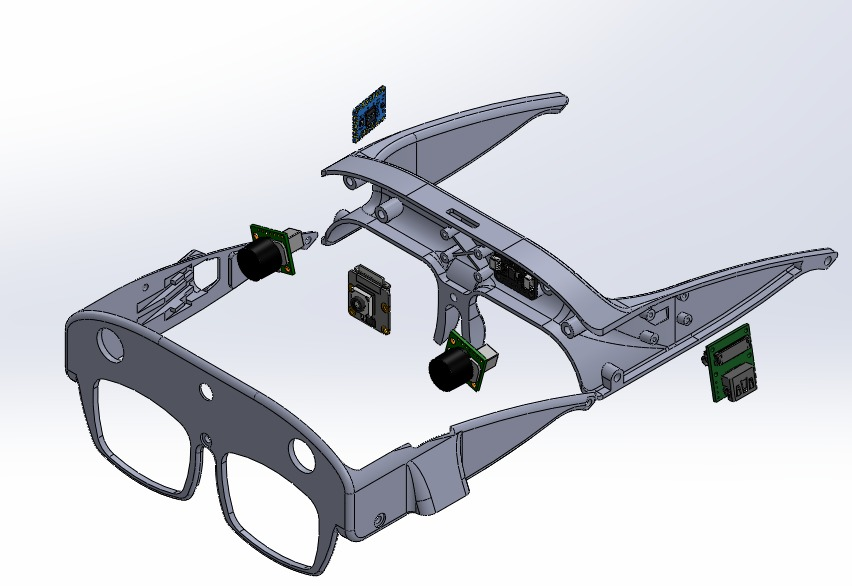
\includegraphics[width=0.85\textwidth]{Capturas_TT2/hardware/Render.jpeg}
    \caption{Vista explosionada del armazón, con la cámara al centro y los sensores
    ultrasónicos sobre cada cristal.}
    \label{fig:proto_explosivo}
\end{figure}

Las Figuras~\ref{fig:proto_transparente} y \ref{fig:proto_armado} muestran el diseño
armado, primero con el frente transparente para ver la disposición interna y después
con el acabado final.

\begin{figure}[H]
    \centering
    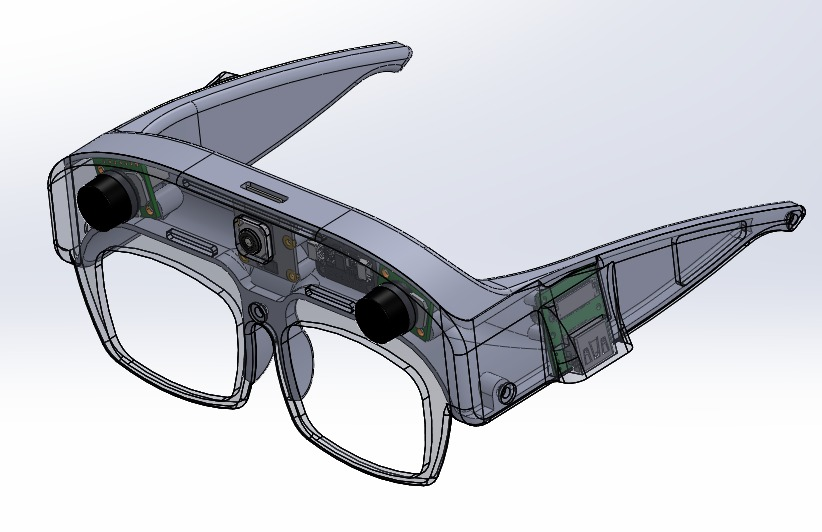
\includegraphics[width=0.8\textwidth]{Capturas_TT2/hardware/VistaPrincipal.jpeg}
    \caption{Diseño armado con el frente transparente.}
    \label{fig:proto_transparente}
\end{figure}

\begin{figure}[H]
    \centering
    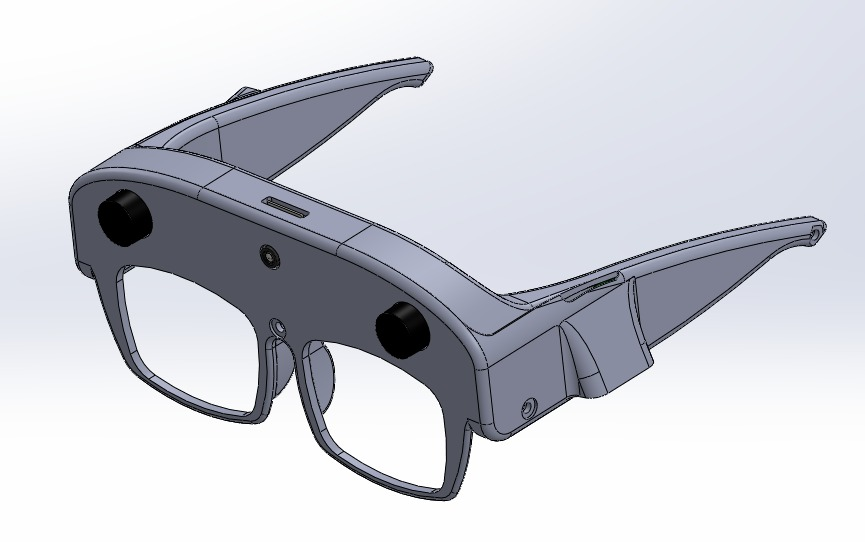
\includegraphics[width=0.8\textwidth]{Capturas_TT2/hardware/VistaReal.jpeg}
    \caption{Diseño armado con el acabado final.}
    \label{fig:proto_armado}
\end{figure}

\TODO{agregar fotos del prototipo fabricado y armado, y describir el material, el
método de fabricación, el peso final y dónde van la Raspberry Pi y la batería}.

Los dos ultrasónicos apuntan hacia adelante, en la misma dirección que la cámara, y
están separados unos 10~cm. Como los sensores y la IMU van en el mismo frente rígido, el
cabeceo que mide la IMU es también el de la cámara y el de los ultrasónicos. Toda esta
geometría se concentra en un solo archivo, \texttt{montaje.py}, que usan el driver de
los sensores, la fusión, las alertas y el simulador, y que se ajusta con las medidas
tomadas sobre el prototipo.

En TT1 se había planteado que los ultrasónicos cubrieran los costados del usuario. Al
revisar la hoja de datos se vio que el MB1232 tiene un haz angosto, de unos
$\pm 14^\circ$, así que sirve poco para vigilar los lados. Puesto al frente, en cambio,
su haz coincide con lo que ve la cámara. Eso permite confirmar o descartar las
detecciones visuales, avisar de vidrios y mamparas que la cámara no reconoce y corregir
el estado de las puertas, como se explica en las secciones de SLAM, visión y alertas.
El costo de esta decisión es que los costados quedan cubiertos solo por la cámara y que
el mapa registra menos superficie lateral (Tabla~\ref{tab:mapeo_us}).


% ==============================================================================
\section{Módulo de visión}
\label{sec:dev_vision}
% ==============================================================================

\subsection{Descripción}

El módulo de visión recibe cada cuadro de la cámara y entrega una lista de
detecciones. Para cada objeto se indica qué es, en qué dirección está respecto al frente
del usuario, a qué distancia aproximada se encuentra, si se está moviendo y, en el caso
de las puertas, si está abierta o cerrada. Con esa lista trabajan el SLAM, las alertas y
la descripción del entorno que el usuario puede pedir por voz. El módulo atiende los
requerimientos RF-07 a RF-10 y RF-13.

En TT1 el módulo se planteó alrededor de un solo detector, YOLOv8. Al probarlo con los
videos reales salió a la luz su mayor carencia, pues el conjunto COCO con el que viene
entrenado no incluye puertas, escaleras ni escritorios, que son justamente los objetos
que más ayudan a orientarse dentro de un edificio. Por eso la versión final combina tres
modelos preentrenados, cada uno con una tarea distinta, como se resume en la
Tabla~\ref{tab:vision_modelos}.

\begin{table}[H]
\centering
\caption{Modelos que componen el módulo de visión}
\label{tab:vision_modelos}
\renewcommand{\arraystretch}{1.25}
\begin{tabular}{|p{3.4cm}|p{3.1cm}|p{2.3cm}|p{5.7cm}|}
\hline
\textbf{Modelo} & \textbf{Entrenamiento} & \textbf{Frecuencia} & \textbf{Uso} \\
\hline
YOLOv8s-seg & COCO, 80 clases & Cada cuadro & Personas, vehículos, muebles y objetos
comunes \cite{redmon2016yolo}. \\
\hline
YOLOv8s & Open Images V7, 600 clases & Cada 5 cuadros (15 en la Raspberry Pi) & Solo
las clases que COCO no tiene, como puerta, escalera, ventana, bote de basura, poste,
letrero, árbol, escritorio, archivero o pizarrón. \\
\hline
SegFormer-B0 & ADE20K, 150 clases & Cada 4 a 10 cuadros & Segmentación de la escena
para encontrar piso transitable, agua, escaleras y puertas \cite{xie2021segformer,
zhou2017ade20k}. \\
\hline
\end{tabular}
\end{table}

\subsection{Preprocesamiento y geometría de la cámara}

Cada cuadro se reduce a 640 píxeles de ancho conservando su relación de aspecto. Una
versión anterior lo forzaba a $640 \times 480$; en los videos 16:9 eso estiraba la
imagen en vertical, inflaba la altura de las cajas y hacía que las distancias salieran
cerca de un 25\,\% más cortas. Ahora la dirección, la distancia por altura típica y la
distancia por plano de piso se calculan con una sola distancia focal, obtenida del campo
de visión horizontal. Hay dos perfiles de cámara, uno para la cámara web de la
computadora portátil ($70^\circ$) y otro para la Camera Module 3 Wide del prototipo
($102^\circ$). Las ecuaciones de distancia se presentan en la Sección~\ref{sec:dev_slam};
el rango estimado se acota entre 0.2 y 8~m.

La igualación de histograma y el filtro gaussiano del pseudocódigo de TT1
(Apéndice~\ref{apend:procesa}) se dejaron fuera. Los modelos preentrenados ya normalizan
la imagen por dentro y, en las pruebas con video, esos pasos no mejoraron nada que
justificara su costo por cuadro.

\subsection{Detección de objetos}

El detector principal es YOLOv8s-seg con un umbral de confianza de 0.45. Algunas
etiquetas de COCO se renombran para que coincidan con el resto del sistema (por ejemplo,
\emph{couch} pasa a \emph{sofa} y \emph{tv} a \emph{monitor}). El detector de Open
Images se ejecuta con un umbral de 0.25 y solo cada cierto número de cuadros, porque en
CPU cuesta casi lo mismo que el principal. De sus 600 clases se conservan nada más las
que aportan algo nuevo, y si una de sus cajas se encima con una de COCO con un IoU mayor
a 0.55, se descarta para no contar dos veces el mismo objeto. La lista de clases creció
después de una prueba en la sala de maestros de la escuela, donde el sistema casi no
detectaba nada porque los escritorios y archiveros no existían en COCO.

\subsection{Puertas, piso y peligros por segmentación}

SegFormer asigna una clase a cada píxel de la imagen, y de ese mapa se sacan tres tipos
de información. La primera son las puertas. Cada región conexa de la clase puerta que
ocupa al menos el 0.4\,\% de la imagen se convierte en una detección, y se considera
abierta si dentro de su recuadro hay más de un 7\,\% de piso transitable, es decir, si a
través del vano se alcanza a ver el piso del otro lado. Cuando el detector de Open
Images ya vio una puerta en la misma dirección (con menos de $8^\circ$ de diferencia),
se conserva solo una. Además, si la puerta queda dentro del haz de los ultrasónicos, el
eco decide su estado, como se explica en la Sección~\ref{sec:dev_slam}.

La segunda son el agua y las escaleras, que ADE20K reconoce como clases propias. Se
toman las regiones que aparecen en el 55\,\% inferior de la imagen y se ubican con la
distancia por plano de piso. La tercera son los hoyos y coladeras, para los que no
existe una clase. Se detectan como regiones no transitables rodeadas de piso, con
varias condiciones para evitar confusiones; la región debe estar en la parte baja de la
imagen, ocupar entre el 0.15 y el 20\,\% del cuadro, no tocar los bordes y estar rodeada
de piso transitable en al menos un 55\,\% de su contorno. Si un peligro coincide en
dirección y distancia con un objeto que ya detectó YOLO, se descarta, porque casi
siempre se trata de la sombra o la base de ese mismo objeto.

\subsection{Objetos en movimiento}

El rastreador de \texttt{vision/motion.py} asocia las cajas entre cuadros y guarda el
historial de sus centroides; si un objeto se desplaza más de 8 píxeles, se marca como
móvil. Las personas, los animales y los vehículos se marcan siempre como móviles. En la
primera versión, cada vez que el usuario giraba la cabeza todo el cuarto parecía
moverse. Para corregirlo, antes de comparar se desplaza el historial del rastreador lo
que corresponde al giro medido por la odometría, $\Delta u = \Delta\theta \cdot W /
\text{FOV}_h$, y así solo queda el movimiento propio de los objetos.

\subsection{Nivel de riesgo}

Cada detección recibe un nivel de riesgo de 0 a 3 según la tabla definida en TT1
(Tabla~\ref{tabla_riesgo}). Los peligros de piso y los objetos en movimiento tienen
riesgo alto (3), los obstáculos estáticos y las puertas cerradas riesgo medio (2), y las
puertas abiertas y las paredes riesgo bajo (1). El mapeo agrupa estos niveles por sector
para construir $r_{\text{front}}$, $r_{\text{left}}$ y $r_{\text{right}}$.

\subsection{Resultados}

La Figura~\ref{fig:vision_escenas} muestra el módulo trabajando sobre tres escenas de
los videos reales. A la izquierda se marcan las detecciones con su distancia estimada
(en verde los objetos estáticos, en rojo los móviles y en magenta los peligros de piso)
y a la derecha la segmentación, con el piso transitable en verde, las puertas en azul y
las paredes en gris.

\begin{figure}[H]
    \centering
    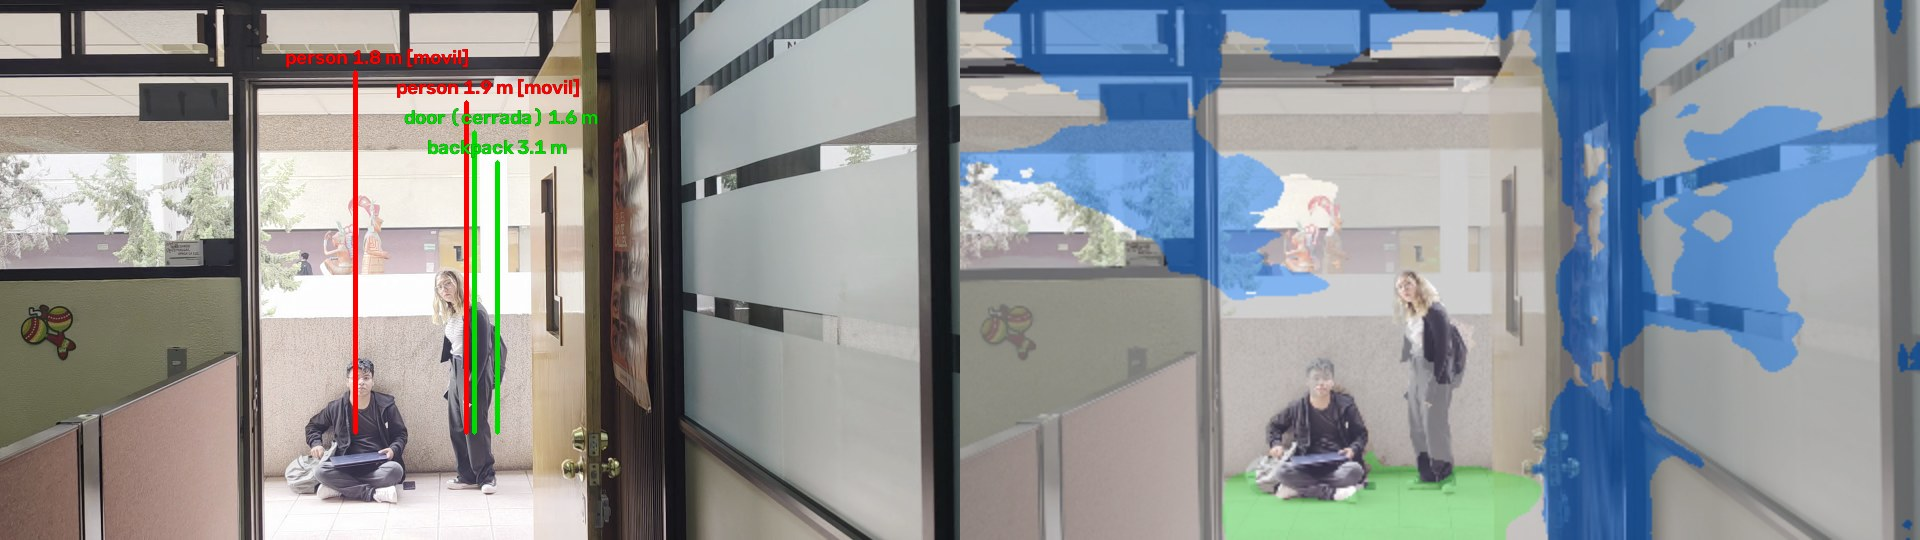
\includegraphics[width=\textwidth]{Capturas_TT2/vision/vision_escena11.jpg}\\[2pt]
    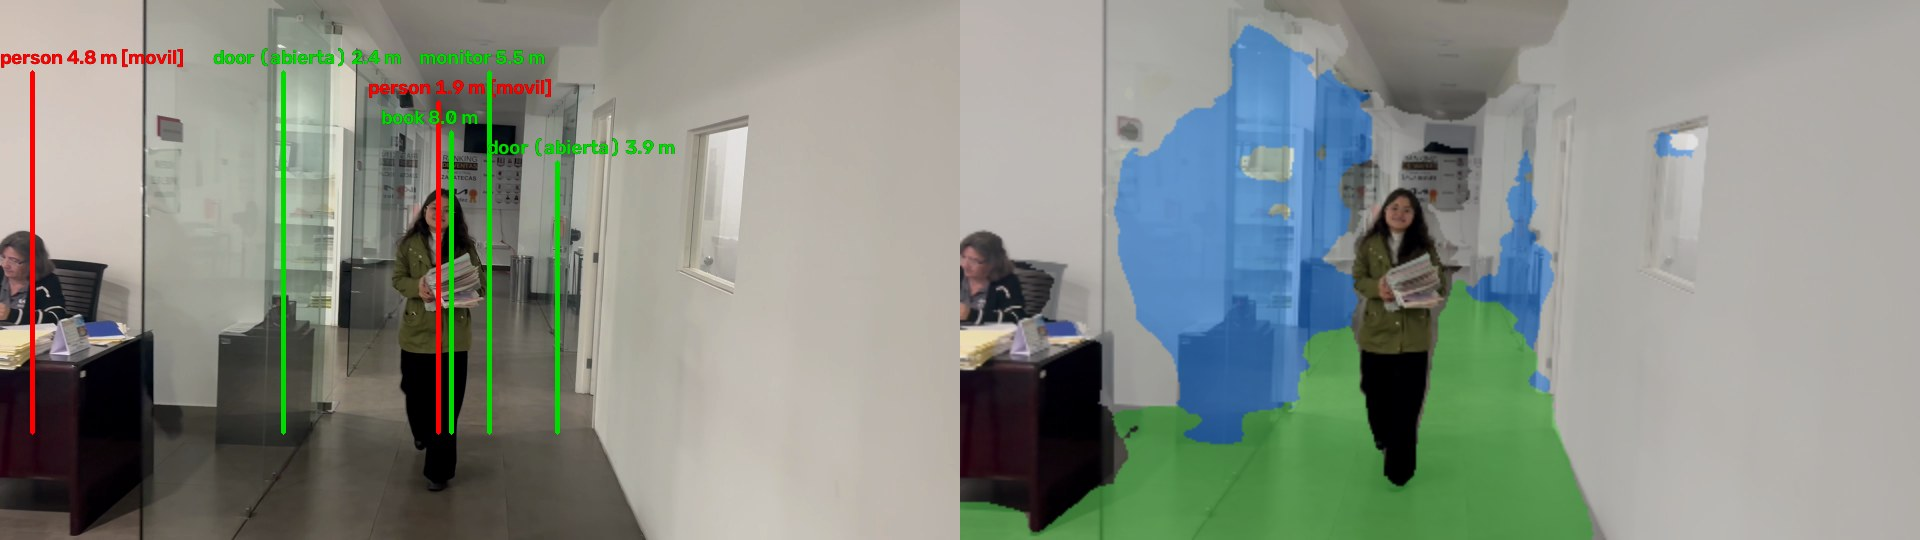
\includegraphics[width=\textwidth]{Capturas_TT2/vision/vision_escena14.jpg}\\[2pt]
    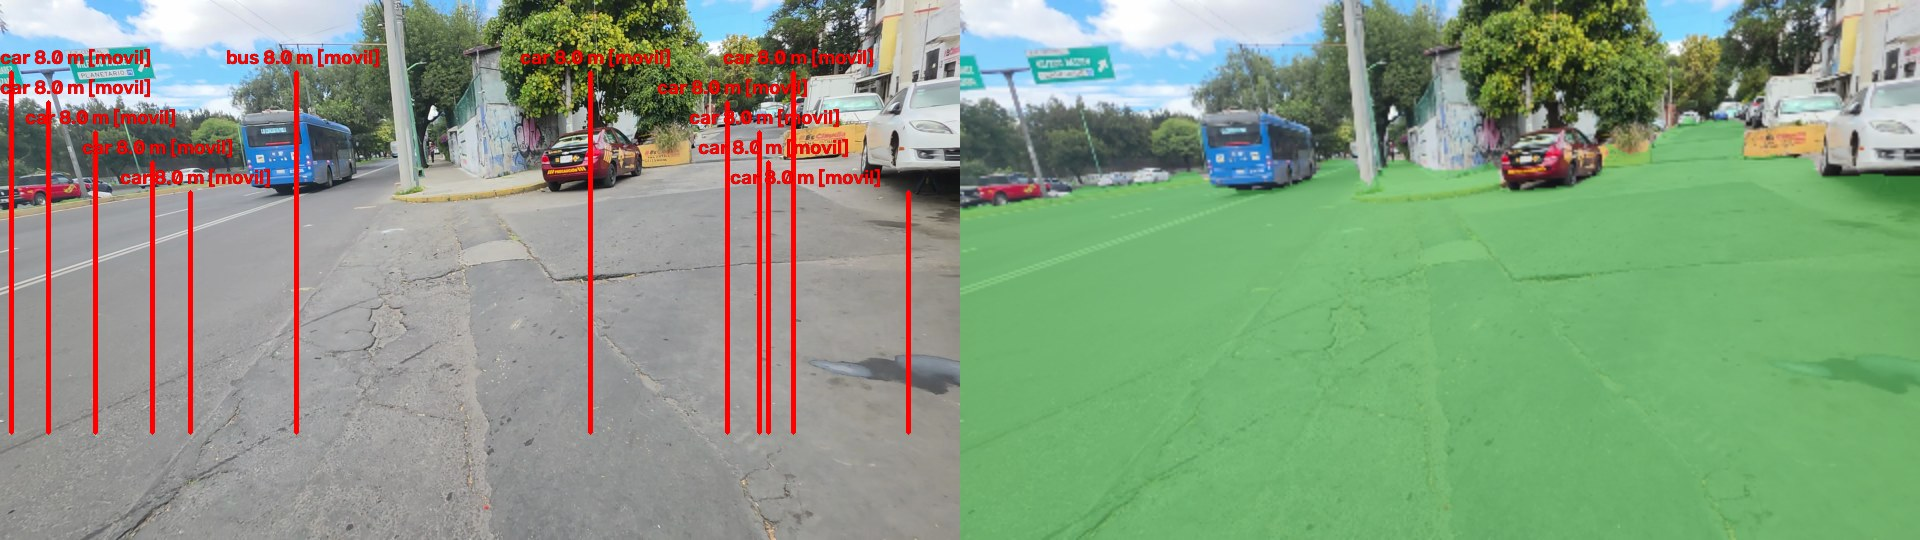
\includegraphics[width=\textwidth]{Capturas_TT2/vision/vision_escena6.jpg}
    \caption{Detecciones (izquierda) y segmentación (derecha) en la entrada de la sala
    de maestros, en un pasillo de oficina con una persona caminando y en una calle con
    vehículos.}
    \label{fig:vision_escenas}
\end{figure}

En la entrada de la sala de maestros el sistema detecta a las dos personas, una mochila
y la puerta, que clasifica como cerrada a 1.6~m. En el pasillo de oficina detecta a la
persona que camina hacia la cámara (a 1.9~m), un monitor y dos puertas abiertas, aunque
la segmentación también marca como puerta buena parte de los canceles de vidrio, así que
al menos una de esas ``puertas'' es en realidad una mampara. La señora sentada en el
escritorio aparece a 4.8~m cuando está a unos 2~m; la distancia se calcula con la altura
típica de una persona de pie (1.65~m), y alguien sentado se ve más bajo, lo que el
modelo interpreta como lejanía. En la calle, los vehículos aparecen como móviles y a
8~m, que es el tope del rango. Más delicado es que la segmentación pinta como piso
transitable tanto la banqueta como el arroyo vehicular, porque la clase \emph{road} de
ADE20K está entre las superficies transitables, y que los baches del pavimento no se
reportan como peligro.

La Figura~\ref{fig:vision_tapete} muestra un falso positivo típico. Un tapete con un
estampado oscuro sobre un piso claro cumple todas las condiciones de un hoyo, porque la
segmentación no lo reconoce como piso, está en la parte baja de la imagen y tiene piso
alrededor. El sistema lo reporta como hoyo a 0.9~m.

\begin{figure}[H]
    \centering
    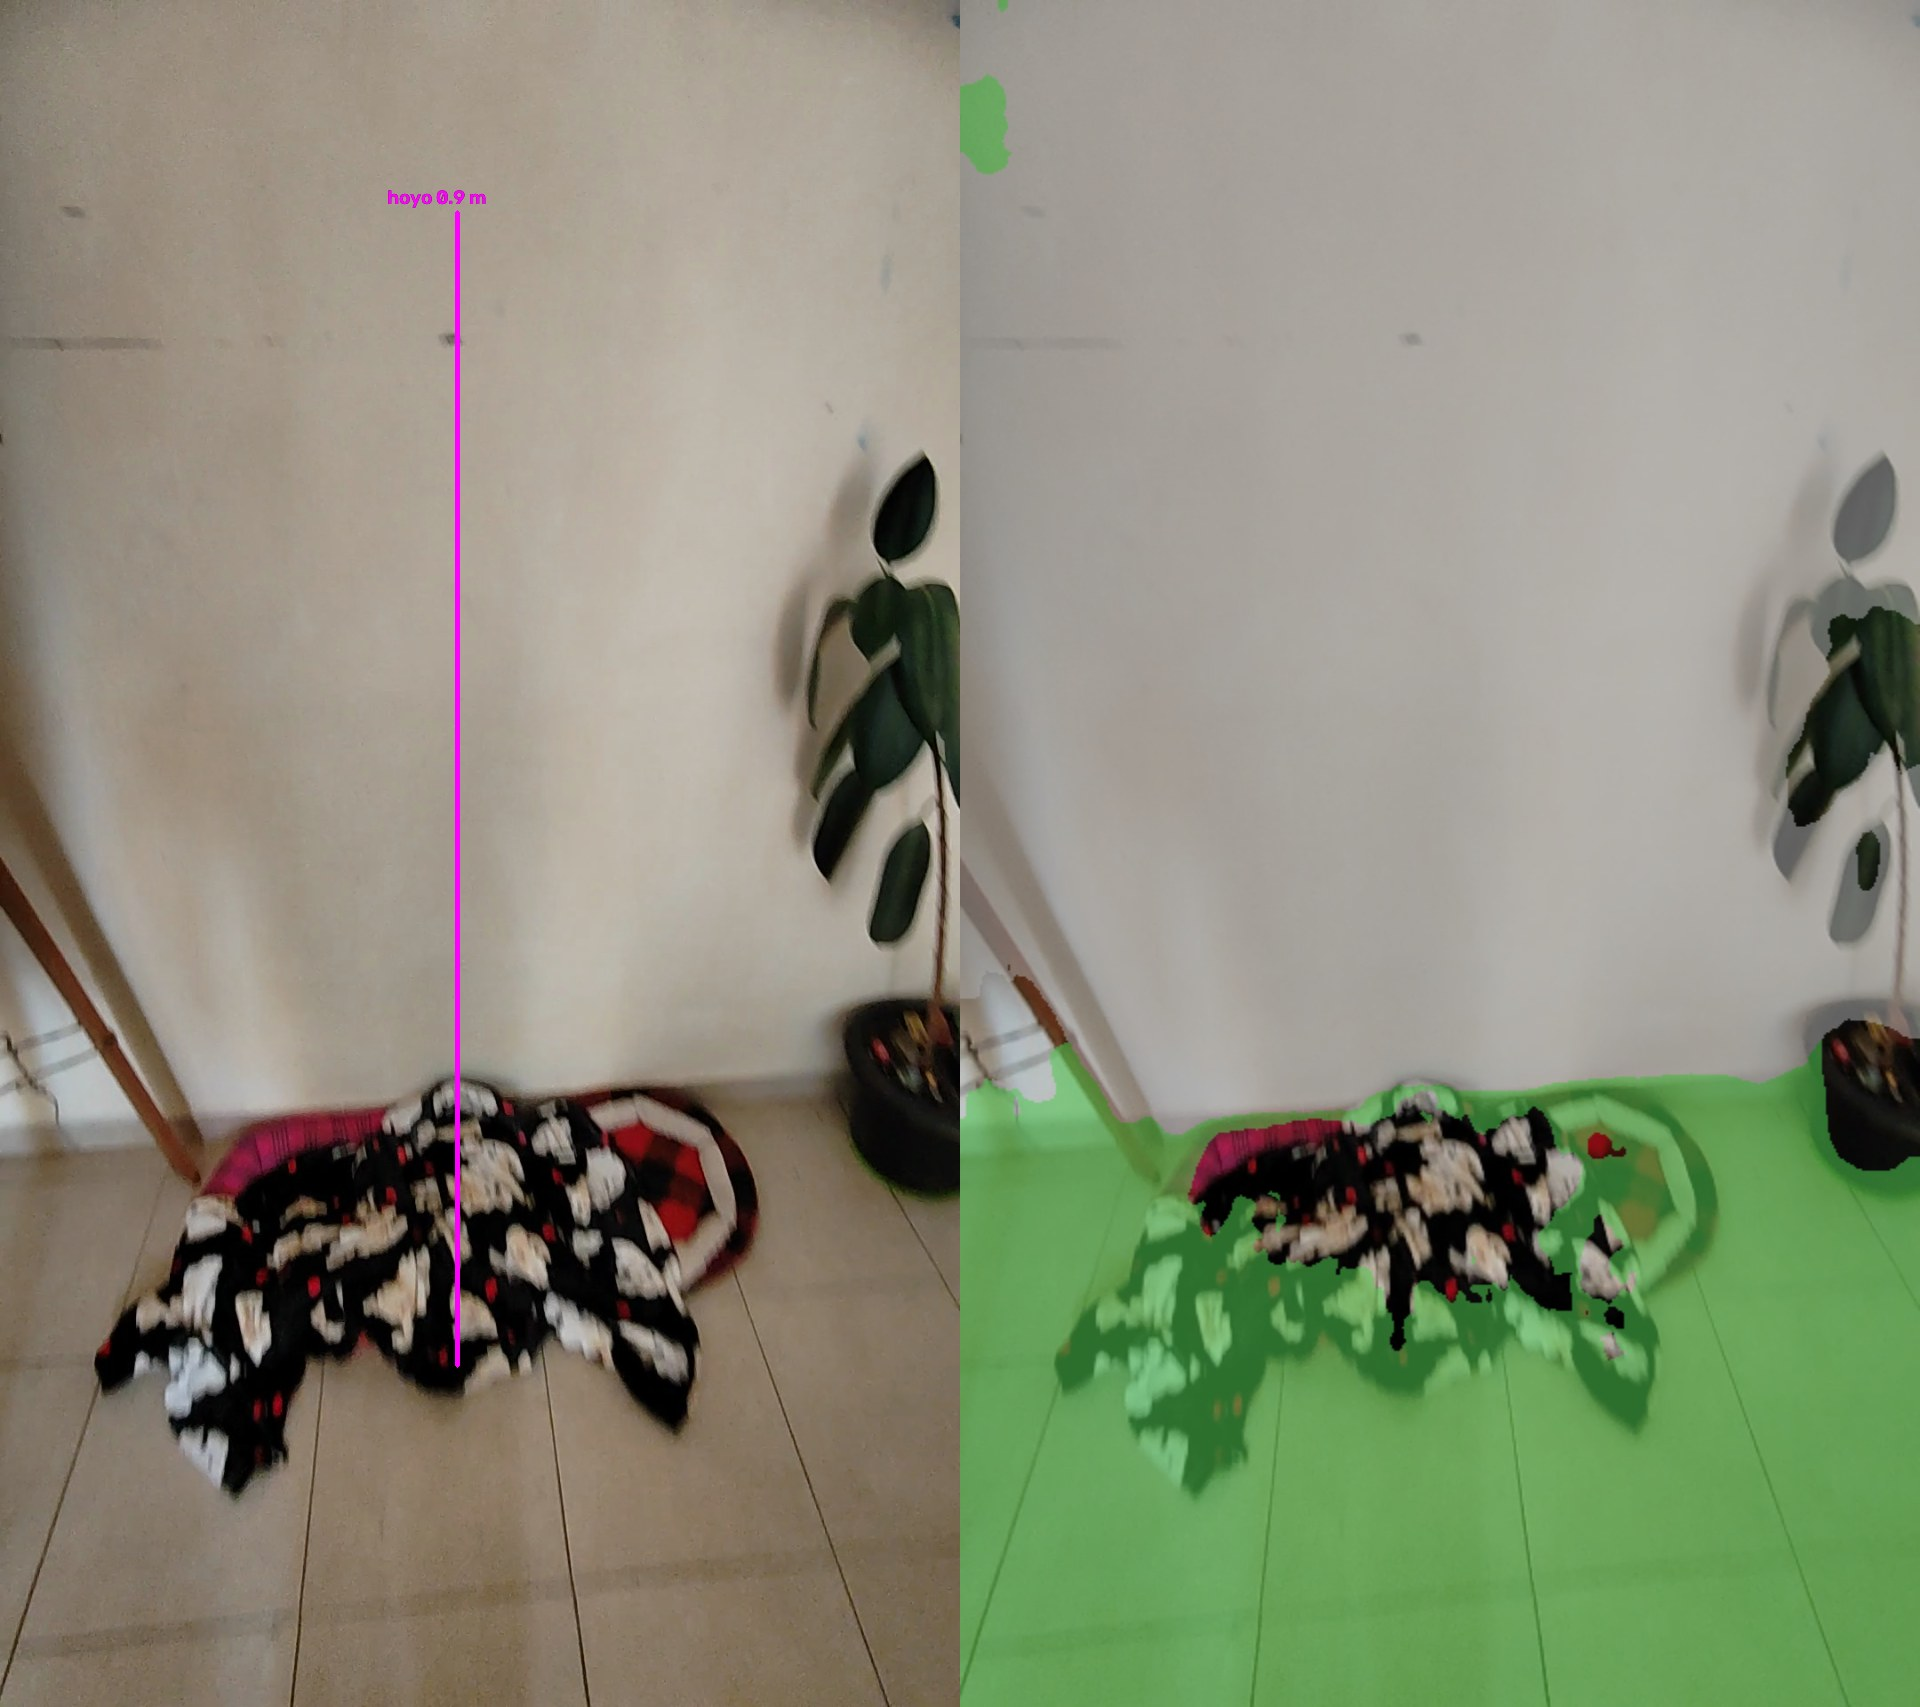
\includegraphics[width=0.62\textwidth]{Capturas_TT2/vision/vision_escena16.jpg}
    \caption{Falso positivo: un tapete estampado se detecta como hoyo a 0.9~m.}
    \label{fig:vision_tapete}
\end{figure}

La Tabla~\ref{tab:vision_tiempos} reporta el tiempo de inferencia de cada modelo,
medido en CPU sobre el mismo cuadro, en la computadora portátil y en la Raspberry Pi del
prototipo.

\begin{table}[H]
\centering
\caption{Tiempo de inferencia por modelo (promedio de 10 ejecuciones)}
\label{tab:vision_tiempos}
\renewcommand{\arraystretch}{1.2}
\begin{tabular}{|l|c|c|c|}
\hline
\textbf{Modelo} & \textbf{Entrada} & \textbf{Apple M4 (ms)} &
\textbf{Raspberry Pi (ms)} \\
\hline
YOLOv8s-seg (COCO) & $640 \times 360$ & 72 & \TODO{} \\
YOLOv8s (Open Images V7) & $640 \times 360$ & 55 & \TODO{} \\
SegFormer-B0 con puertas y peligros & $480 \times 270$ & 293 & \TODO{} \\
\hline
\end{tabular}
\end{table}

En la computadora portátil, con el detector principal en cada cuadro, el extra cada
cinco y la segmentación cada cuatro, el costo promedio es de unos 160~ms por cuadro, o
sea, unos 6 cuadros por segundo. La segmentación es lo más caro; por eso se ejecuta con
menos frecuencia y sus resultados se reutilizan en los cuadros intermedios. En la
Raspberry Pi, con la configuración del prototipo (extra cada 15 cuadros y segmentación
cada 10), el sistema procesa \TODO{cuadros por segundo en la Raspberry Pi}.

La precisión de detección que pide RNF-06 se mide sobre imágenes tomadas con la
cámara del prototipo y etiquetadas a mano. \TODO{armar el conjunto y reportar número de
imágenes, clases, precisión y exhaustividad}. Para mejorar las clases propias del
entorno se cuenta con el script \texttt{vision/finetune.py}, que reentrena YOLO con un
conjunto en formato YOLO. \TODO{resultado del reentrenamiento con puertas y mamparas de
la escuela, si se realiza}. El módulo tiene 15 pruebas automatizadas que usan detectores
simulados para revisar la geometría, las puertas, el detector extra y la eliminación de
duplicados.

\subsection{Limitaciones}

Ninguno de los tres modelos tiene una clase para mamparas o canceles de vidrio. La
segmentación a veces los toma por puertas y a veces no los ve; los ultrasónicos
frontales compensan en parte, porque un eco sin detección visual se avisa como pared y
el eco corrige el estado de las puertas de vidrio, pero solo dentro de su cono angosto.
El criterio geométrico de los hoyos también genera falsos positivos con tapetes,
manchas y cambios de textura del piso.

El rastreador compensa el giro del usuario, pero no su avance. Al caminar hacia
adelante, las cajas de los objetos cercanos crecen y algunos objetos estáticos se marcan
como móviles, como se ve en la Figura~\ref{fig:cap_oficina_3}. La distancia monocular,
por su parte, depende de la altura típica de cada clase, de modo que una persona sentada
o un objeto de tamaño poco común quedan mal ubicados, y se satura en 8~m. Por último, la
calle se considera tan transitable como la banqueta y los baches poco profundos no se
distinguen del pavimento, así que en exteriores el sistema no sabe por sí solo que bajar
al arroyo vehicular es peligroso. \TODO{separar banqueta y arroyo vehicular en la
segmentación}.


% ==============================================================================
\section{Módulo de SLAM}
\label{sec:dev_slam}
% ==============================================================================

\subsection{Descripción y alcance}

El módulo de SLAM responde en cada ciclo una pregunta sencilla de plantear y difícil de
resolver, que es dónde está el usuario y hacia dónde mira dentro del mapa que se va
construyendo. Ningún sensor entrega esa respuesta de manera directa. La cámara da la
dirección de los objetos con buena precisión, pero su distancia con mucho error; el
ultrasonido mide distancias exactas, pero solo hacia el frente; y cualquier estimación
de movimiento acumula error con el tiempo. El SLAM junta estas fuentes, lleva la cuenta
de qué tanto se puede confiar en la pose y la entrega a los módulos de Ray Casting y
mapeo. Con ello cubre RF-14 y RF-15.

En TT1 se planteó un SLAM ``simplificado'' basado en un filtro de Kalman extendido
(EKF) \cite{kalman1960, thrun2005probabilistic}, y esa idea se mantuvo, aunque hubo que
precisar la variante. En el EKF-SLAM clásico \cite{smith1990uncertain} el vector de
estado incluye la pose y la posición de cada \emph{landmark}, de modo que la matriz de
covarianza crece con el cuadrado del número de elementos del mapa
\cite{bailey2006slam2}. Los sistemas de SLAM visual como ORB-SLAM
\cite{murartal2015orbslam}, por su parte, siguen miles de puntos característicos y
piden más cómputo del que una Raspberry Pi puede dar mientras también ejecuta la
detección de objetos.

Por eso el estado del filtro contiene solo la pose, $\boldsymbol{\mu} = [x,\; y,\;
\theta]^T$, con una covarianza $\mathbf{P}$ de $3 \times 3$, y el costo de cada ciclo es
el mismo sin importar cuántos objetos haya en el mapa. Los \emph{landmarks} se guardan
en una lista ligera fuera del filtro, cada uno con su posición, su etiqueta (silla,
puerta, mesa, etc.) y el número de veces que se ha visto. Al corregir, el filtro usa el
\emph{landmark} asociado como referencia y suma su incertidumbre de posición, que baja
con cada nueva observación, a la covarianza de la innovación; así no trata a un objeto
recién visto como si su posición fuera exacta. En términos académicos, la variante
corresponde a un EKF de localización con mapeo incremental de apoyo. Se privilegia una
pose barata y estable, y el mapa de ocupación lo refinan después los módulos de Ray
Casting y mapeo con la pose que el SLAM les entrega.

\subsection{Entradas y salidas}

La Tabla~\ref{tab:slam_interfaces} describe las estructuras de datos que intercambia el
módulo, definidas en \texttt{interfaces.py}.

\begin{table}[H]
\centering
\caption{Interfaces del módulo de SLAM}
\label{tab:slam_interfaces}
\renewcommand{\arraystretch}{1.25}
\begin{tabular}{|p{3.3cm}|p{1.6cm}|p{9.6cm}|}
\hline
\textbf{Estructura} & \textbf{Tipo} & \textbf{Contenido} \\
\hline
\texttt{MotionEstimate} & Entrada & Desplazamiento $\Delta d$ (m), giro $\Delta\theta$
(rad) e intervalo $\Delta t$ (s) desde el ciclo anterior. \\
\hline
\texttt{Observation} & Entrada & Rango $r$ (m), dirección $\phi$ relativa al frente
del usuario (rad, positiva hacia la izquierda), etiqueta, desviaciones estándar propias
$\sigma_r$ y $\sigma_\phi$, y banderas que indican si la observación puede crear
\emph{landmarks}, si puede corregir la pose y si es un peligro de piso. \\
\hline
\texttt{SlamOutput} & Salida & Pose $(x, y, \theta)$, covarianza de $3 \times 3$,
marca de tiempo y confianza entre 0 y 1. \\
\hline
Lista de \emph{landmarks} & Salida & Posición, etiqueta, número de avistamientos y
estado (candidato o confirmado) de cada elemento del mapa ligero. \\
\hline
\end{tabular}
\end{table}

Como ejemplo, la salida de un ciclo, tal como la recibe el resto del sistema, se ve así.

\begin{verbatim}
pose: {x: 1.83, y: 0.42, theta: 0.31}
covarianza: [[0.0021, 0.0001, 0.0000],
             [0.0001, 0.0019, 0.0000],
             [0.0000, 0.0000, 0.0007]]
timestamp: 1737657000.231
confianza: 0.94
\end{verbatim}

\subsection{Fuentes de movimiento}

Para la predicción hace falta saber cuánto avanzó y cuánto giró el usuario desde el
ciclo anterior. El módulo \texttt{odometry.py} obtiene ese dato de tres maneras, en
orden de preferencia.

La fuente principal es la IMU BNO055 de Bosch \cite{bno055_datasheet}, conectada al
mismo bus I2C que los ultrasónicos y configurada en su modo de fusión NDOF, en el que
el propio chip combina acelerómetro, giroscopio y magnetómetro. El giro de cada ciclo es
la diferencia entre dos lecturas del rumbo fusionado. Para el avance no se integra la
aceleración dos veces, porque el error crecería con el cuadrado del tiempo; se usa en
cambio la navegación peatonal por estima (\emph{pedestrian dead reckoning})
\cite{harle2013pdr}. Cada paso se detecta como un pico en la magnitud de la aceleración
lineal por encima de 1.8~m/s$^2$, con rearme cuando baja de 0.8~m/s$^2$ y un mínimo de
0.3~s entre pasos, y cada paso suma una longitud configurable, de 0.68~m por defecto. La
IMU también mide la inclinación real de la cabeza, que se usa para la distancia por
plano de piso. Como la orientación del chip dentro del armazón puede variar, se
configura con las posiciones de montaje P0 a P7 de su hoja de datos, y el programa
\texttt{odometry.py --calibrar} identifica, con los lentes puestos, qué eje corresponde
al cabeceo, su signo y su cero.

Si la IMU no responde, el sistema pasa solo al flujo óptico de la cámara. Se eligen
puntos característicos con el detector de Shi--Tomasi \cite{shi1994good}, se siguen
entre cuadros con el método de Lucas--Kanade \cite{lucas1981iterative} y el giro se
calcula con la mediana del desplazamiento horizontal, $\Delta\theta =
\arctan(\overline{\Delta u} / f)$, donde $f$ es la distancia focal en píxeles. En este
modo no se estima el avance.

La tercera fuente solo se usa al procesar videos grabados, que no traen información
inercial. Al flujo óptico se le resta la parte que corresponde al giro, y si lo que
queda supera 1.4 píxeles se considera que el usuario está caminando, con una velocidad
supuesta de 1.1~m/s. Con esto se pueden construir mapas a partir de videos, aunque su
escala depende de esa velocidad.

\subsection{Construcción de observaciones}

La función \texttt{fuseObservations} convierte las detecciones de la cámara y las
lecturas ultrasónicas en observaciones de rango y dirección. La dirección de un objeto
sale de la columna central de su caja y del campo de visión de la cámara. La distancia
se estima con el modelo de cámara estenopeica \cite{hartley2004multiple}:

\[
d_{h} = \frac{f \, H_{\text{típica}}}{h_{\text{bbox}}},
\qquad
f = \frac{W/2}{\tan(\text{FOV}_h/2)}
\]

donde $H_{\text{típica}}$ es la altura típica de la clase (1.65~m para una persona,
0.90~m para una silla o 2.00~m para una puerta, por ejemplo) y $h_{\text{bbox}}$ es la
altura de la caja en píxeles. Si el borde inferior de la caja se ve en la imagen, se
calcula además la distancia al punto donde el objeto toca el piso:

\[
d_{g} = \frac{h_{c}}{\tan\!\left(\alpha + \arctan\dfrac{v_b - H/2}{f}\right)}
\]

con $h_c = 1.55$~m como altura de la cámara, $\alpha$ como su inclinación hacia el piso
(10° por defecto, o la que mide la IMU) y $v_b$ como la fila del borde inferior. El
resultado final es $d_g$, pero acotado entre $0.4\,d_h$ y $1.6\,d_h$, lo que combina la
estabilidad del primer modelo con la mejor precisión del segundo.

Cada observación lleva su propia incertidumbre y el filtro la usa para dar más o menos
peso a cada fuente, sin necesidad de casos especiales. La Tabla~\ref{tab:slam_fusion}
resume las reglas.

\begin{table}[H]
\centering
\caption{Reglas de construcción de observaciones y su incertidumbre}
\label{tab:slam_fusion}
\renewcommand{\arraystretch}{1.25}
\begin{tabular}{|p{4.3cm}|p{2.4cm}|p{1.6cm}|p{5.9cm}|}
\hline
\textbf{Caso} & $\sigma_r$ & $\sigma_\phi$ & \textbf{Uso} \\
\hline
Detección visual con eco ultrasónico compatible & 0.05~m & $3^\circ$ & Rango del
ultrasonido y dirección de la cámara. Corrige la pose y crea \emph{landmarks} con 2
avistamientos. \\
\hline
Detección visual sin respaldo & $0.30\,r$ & $3^\circ$ & Corrige la pose; hacen falta 4
avistamientos para confirmar un \emph{landmark}. \\
\hline
Peligro de piso (hoyo, agua, escalera) & $0.20\,r$ & $3^\circ$ & Va a la capa de
peligros del mapa. \\
\hline
Eco ultrasónico sin detección visual & 0.05~m & $10^\circ$ & Solo actualiza el mapa;
no corrige la pose ni crea \emph{landmarks}. \\
\hline
Objeto en movimiento & --- & --- & Se descarta, porque una persona caminando no es una
referencia fija. \\
\hline
\end{tabular}
\end{table}

Una detección y un eco se toman como el mismo objeto si sus direcciones difieren menos
de $20^\circ$ y sus rangos son compatibles, es decir, si
$|r_{us} - r_{mono}| \leq \max(0.6,\; 0.5\, r_{mono})$.

\textbf{Ecos de pared.} En una primera versión, los ecos que no tenían una detección
visual asociada también creaban \emph{landmarks} y corregían la pose. El problema es que
el punto donde rebota un eco sobre una pared se desliza conforme el usuario camina, así
que no es un punto fijo del mundo, y usarlo como referencia echaba a perder la pose. Al
sacar esos ecos de la corrección, el ATE promedio del banco bajó de 0.53 a 0.27~m. Los
ecos se siguen enviando siempre al mapa de ocupación, porque el extremo de cada rayo sí
cae sobre la superficie que lo produjo.

\textbf{Ultrasonido frontal y validación cruzada.} Los dos MB1232 del prototipo van al
frente, uno sobre cada cristal, separados unos 10~cm y apuntando en la misma dirección
que la cámara (Sección~\ref{sec:dev_prototipo}). Según su hoja de datos son sensores de
haz angosto, con un cono útil de unos $\pm 14^\circ$, y su alcance depende del tamaño
del objeto; alimentados a 3.3~V, como en la Raspberry Pi, detectan a una persona hasta a
1.8~m y una pared hasta a unos 6~m \cite{mb1232_datasheet}. Sobre este montaje se
construyeron cuatro mecanismos.

El primero es geométrico. Cada lectura se convierte a coordenadas polares centradas en
la cámara, tomando en cuenta el desplazamiento lateral de su sensor, antes de
fusionarla. El segundo aprovecha que los dos sensores ven casi lo mismo, pues cuando
ambos detectan el mismo objeto, la diferencia entre sus rangos indica de qué lado está,
con $y = (r_{der}^2 - r_{izq}^2)/2s$, donde $s$ es la separación, y una zona muerta de
5~cm para no reaccionar al ruido.

El tercero es la validación cruzada, que corresponde al Algoritmo 2 de TT1. Si una
detección visual cae dentro del cono y hay un eco compatible, se marca como confirmada
por ambos sensores y toma el rango del ultrasonido, que es mucho más preciso. Si el haz
debería alcanzar al objeto, por su tamaño, su altura y su distancia, pero el eco está
mucho más lejos, la detección se marca como contradicha. Con las puertas el criterio
sirve también para saber su estado, ya que un eco que pasa por el vano indica que está
abierta y uno a la distancia de la puerta, que está cerrada; esto corrige las puertas de
vidrio que la segmentación daba por abiertas. El cuarto mecanismo descarta los ecos del
piso. Cuando el usuario inclina la cabeza, el haz rebota en el suelo; con el cabeceo de
la IMU se calcula a qué distancia lo toca, y esas lecturas se tratan como espacio libre
y no como pared.

Como los dos sensores apuntan al mismo lado, si disparan a la vez cada uno escucha el eco
del otro. Por eso el driver los dispara de forma alternada en un hilo propio, con
100~ms entre la orden de medir y la lectura, como indica la hoja de datos.

\subsection{Predicción}

La pose se propaga con un modelo de arco, en el que el avance se aplica en la
orientación promedio del tramo. Es más exacto que aplicarlo en la orientación inicial
cuando el usuario gira mientras camina.

\[
\theta_m = \theta + \frac{\Delta\theta}{2},
\qquad
\begin{bmatrix} x' \\ y' \\ \theta' \end{bmatrix}
=
\begin{bmatrix}
x + \Delta d \cos\theta_m \\
y + \Delta d \sin\theta_m \\
\operatorname{wrap}(\theta + \Delta\theta)
\end{bmatrix}
\]

El jacobiano respecto al estado y la propagación de la covarianza quedan como sigue.

\[
\mathbf{G} =
\begin{bmatrix}
1 & 0 & -\Delta d \sin\theta_m \\
0 & 1 & \Delta d \cos\theta_m \\
0 & 0 & 1
\end{bmatrix},
\qquad
\mathbf{P}' = \mathbf{G}\,\mathbf{P}\,\mathbf{G}^T + \mathbf{Q}
\]

El ruido de proceso crece con el movimiento, con
$\mathbf{Q} = \operatorname{diag}(\sigma_t^2,\, \sigma_t^2,\, \sigma_\theta^2)$,
$\sigma_t = 0.02 + 0.05\,|\Delta d|$~m y
$\sigma_\theta = 0.035\,\max(|\Delta\theta|,\, 0.01) + 0.3^\circ$. La covarianza
inicial es $\operatorname{diag}(0.01,\; 0.01,\; (1^\circ)^2)$, porque el sistema arranca
en el origen de su propio marco de referencia.

\subsection{Modelo de observación y asociación de datos}

Para un \emph{landmark} conocido en $(l_x, l_y)$, la observación esperada y su
jacobiano son los siguientes.

\[
\delta_x = l_x - x,\quad \delta_y = l_y - y,\quad q = \delta_x^2 + \delta_y^2
\]
\[
\hat{\mathbf{z}} =
\begin{bmatrix} \sqrt{q} \\ \operatorname{atan2}(\delta_y, \delta_x) - \theta
\end{bmatrix},
\qquad
\mathbf{H} =
\begin{bmatrix}
-\delta_x/\sqrt{q} & -\delta_y/\sqrt{q} & 0 \\
\delta_y/q & -\delta_x/q & -1
\end{bmatrix}
\]

Cada observación $\mathbf{z} = [r, \phi]^T$ se asocia con el \emph{landmark} confirmado
más cercano en distancia de Mahalanobis, siempre que esa distancia quede por debajo de un
umbral de compuerta \cite{barshalom2001estimation, neira2001jcbb}.

\[
\boldsymbol{\nu} = \mathbf{z} - \hat{\mathbf{z}},
\qquad
\mathbf{S} = \mathbf{H}\mathbf{P}\mathbf{H}^T + \mathbf{R} + \mathbf{R}_{lm},
\qquad
d^2 = \boldsymbol{\nu}^T \mathbf{S}^{-1} \boldsymbol{\nu} < \gamma^2,\quad \gamma = 3
\]

Aquí $\mathbf{R} = \operatorname{diag}(\sigma_r^2, \sigma_\phi^2)$ viene de la propia
observación y $\mathbf{R}_{lm}$ representa la incertidumbre del \emph{landmark}, con
$\sigma_{lm} = 0.4/\sqrt{n}$~m para un elemento visto $n$ veces. Además, solo se comparan
etiquetas compatibles, así que una silla nunca se asocia con una mesa. Las etiquetas
genéricas, como la de un eco sin clase, son compatibles con todas y toman la etiqueta
correcta en cuanto la cámara identifica al objeto.

\subsection{Corrección}

Si hay asociación, se calcula la ganancia de Kalman y se actualizan la pose y la
covarianza. Para la covarianza se usa la forma de Joseph, que es más estable
numéricamente que la forma simplificada y mantiene a $\mathbf{P}$ simétrica y
semidefinida positiva \cite{grewal2015kalman}.

\[
\mathbf{K} = \mathbf{P}\mathbf{H}^T\mathbf{S}^{-1},
\qquad
\boldsymbol{\mu} \leftarrow \boldsymbol{\mu} + \mathbf{K}\boldsymbol{\nu}
\]
\[
\mathbf{P} \leftarrow (\mathbf{I} - \mathbf{K}\mathbf{H})\,\mathbf{P}\,
(\mathbf{I} - \mathbf{K}\mathbf{H})^T + \mathbf{K}\mathbf{R}_{ef}\mathbf{K}^T
\]

donde $\mathbf{R}_{ef} = \mathbf{R} + \mathbf{R}_{lm}$. Después de cada corrección se
impone un mínimo a la varianza de cada componente ($10^{-4}$~m$^2$ en posición y
$(0.5^\circ)^2$ en orientación). Sin ese mínimo, tras miles de correcciones el filtro
terminaría creyendo que su pose es perfecta y dejaría de reaccionar a observaciones
nuevas, lo cual sería grave si el usuario tropieza o alguien lo mueve.

Si en un ciclo ninguna observación se asocia, no hay corrección y el sistema sigue solo
con la predicción. La confianza que se reporta combina la incertidumbre con el número
$k$ de ciclos seguidos sin corrección,

\[
c = \frac{1}{1 + \operatorname{tr}(\mathbf{P})}\cdot 0.9^{k},
\]

de modo que el módulo de navegación sabe cuándo la pose es menos fiable y puede actuar
con más cuidado, como pide RNF-09.

\subsection{Gestión de \emph{landmarks}}

Una observación que no se asocia con ningún \emph{landmark} confirmado no se tira; pasa
a alimentar el mapa ligero. Primero se proyecta al marco global y se busca un candidato
que corresponda al mismo objeto. La comparación usa la elipse de incertidumbre de la
observación, que es estrecha en dirección y alargada en profundidad, y gracias a ella la
misma silla vista a 2.1~m y después a 2.9~m (con el $\pm 30$\,\% de error de la
estimación monocular) se reconoce como un solo objeto. Si no hay candidato, se crea uno
nuevo.

El candidato se confirma tras 2 avistamientos si tiene respaldo del ultrasonido, o tras
4 si solo lo vio la cámara. Así, un falso positivo de YOLO que aparece en uno o dos
cuadros no se convierte en un obstáculo inventado. La observación que confirma a un
candidato no corrige la pose en ese mismo ciclo, para no contar dos veces la misma
evidencia. Cada vez que el objeto se vuelve a ver, su posición se acerca a la nueva
medición con un factor $\alpha = \max(0.05,\; 1/n)$, que al principio equivale a un
promedio acumulado y, cuando el objeto ya se vio muchas veces, a un promedio móvil. Los
candidatos que no se vuelven a ver en 40 ciclos se eliminan, y dos \emph{landmarks}
confirmados con la misma etiqueta a menos de 0.7~m se funden en uno, ponderando por sus
avistamientos, para deshacer duplicados causados por la deriva.

Por último, la función \texttt{observationsForMap} cambia el rango crudo de cada
observación asociada por la posición consolidada de su \emph{landmark}, con
$\sigma_r = 0.05$~m. Con eso cada objeto deja en el mapa de ocupación una marca firme en
la misma celda, en lugar de una mancha dispersa por el ruido monocular; solo se anclan
los \emph{landmarks} con una etiqueta real. Los \emph{landmarks} confirmados se pueden
guardar y volver a cargar en otra sesión (\texttt{exportLandmarks} e
\texttt{importLandmarks}), y así el filtro puede corregir contra un lugar conocido desde
el primer ciclo.

\subsection{Pseudocódigo del ciclo implementado}

El Algoritmo~\ref{alg:dev_slam} resume un ciclo completo del módulo, tal como quedó en
el método \texttt{EKFSlam.step}.

\begin{center}
\captionof{algorithm}{Ciclo del módulo SLAM implementado}
\label{alg:dev_slam}
\end{center}
\vspace{-1.8cm}
\rule{\textwidth}{0.4pt}
\vspace{-0.9cm}
\begin{algorithmic}[1]

\Statex \textbf{ENTRADA:}
\Statex movimiento \Comment{($\Delta d$, $\Delta\theta$, $\Delta t$)}
\Statex observaciones \Comment{lista de (r, $\phi$, etiqueta, $\sigma_r$, $\sigma_\phi$, banderas)}
\Statex \textbf{SALIDA:}
\Statex salida\_slam \Comment{pose, covarianza, marca de tiempo, confianza}

\Statex
\Statex \textbf{--- ETAPA 1: PREDICCIÓN ---}
\State $\theta_m \gets \theta + \Delta\theta / 2$
\State $x \gets x + \Delta d \cos\theta_m$;\; $y \gets y + \Delta d \sin\theta_m$
\State $\theta \gets$ normalizar($\theta + \Delta\theta$)
\State $\mathbf{P} \gets \mathbf{G}\mathbf{P}\mathbf{G}^T + \mathbf{Q}(\Delta d, \Delta\theta)$

\Statex
\Statex \textbf{--- ETAPA 2: CORRECCIÓN ---}
\State hubo\_correccion $\gets$ falso
\For{cada obs en observaciones}
    \If{obs no es válida}
        \State continuar
    \EndIf
    \If{obs.puede\_corregir es falso}
        \State guardar obs solo para el mapa
        \State continuar
    \EndIf
    \State ref, $\mathbf{H}$, $\mathbf{S}$, $\boldsymbol{\nu}$ $\gets$
    asociar(obs) \Comment{Mahalanobis $< 3$ y etiqueta compatible}
    \If{no se encontró ref}
        \If{obs.puede\_crear\_referencia}
            \State actualizar\_candidato(obs) \Comment{crea, refina o confirma}
        \EndIf
        \State continuar
    \EndIf
    \State $\mathbf{K} \gets \mathbf{P}\mathbf{H}^T\mathbf{S}^{-1}$
    \State $\boldsymbol{\mu} \gets \boldsymbol{\mu} + \mathbf{K}\boldsymbol{\nu}$;\;
    normalizar $\theta$
    \State $\mathbf{P} \gets$ forma\_de\_Joseph($\mathbf{P}$, $\mathbf{K}$, $\mathbf{H}$, $\mathbf{R}_{ef}$)
    \State aplicar varianza mínima a $\mathbf{P}$
    \State refinar posición de ref;\; ref.avistamientos $\gets$ ref.avistamientos + 1
    \State hubo\_correccion $\gets$ verdadero
\EndFor

\Statex
\Statex \textbf{--- ETAPA 3: MANTENIMIENTO ---}
\If{hubo\_correccion}
    \State $k \gets 0$
\Else
    \State $k \gets k + 1$ \Comment{ciclos solo con predicción}
\EndIf
\State eliminar candidatos no vistos en 40 ciclos
\State fundir referencias confirmadas iguales a menos de 0.7 m
\State confianza $\gets 0.9^{k} / (1 + \operatorname{tr}(\mathbf{P}))$

\Statex
\State \Return (x, y, $\theta$, $\mathbf{P}$, tiempo\_actual(), confianza)

\end{algorithmic}
\vspace{-0.9cm}
\rule{\textwidth}{0.4pt}

\subsection{Resultados}

\textbf{Pruebas con el prototipo.} \TODO{error de posición medido con el prototipo en
un recorrido de longitud conocida (por ejemplo, un pasillo marcado en el piso),
número de \emph{landmarks} confirmados y estado de calibración de la IMU}.

\textbf{Exactitud en el banco de simulación.} La Figura~\ref{fig:slam_trayectorias}
muestra un recorrido de 300 ciclos por el cuarto simulado, con la trayectoria real, la
estimada por el EKF y la que resultaría de integrar solo la odometría. Las elipses
representan dos desviaciones estándar de la posición; crecen mientras el usuario no ve
objetos conocidos y se encogen al volver a verlos. También aparece un \emph{landmark}
junto a la pared derecha (cerca de $x = 5.9$~m) que no corresponde a ningún objeto real
y que es producto del error de la distancia monocular.

\begin{figure}[H]
    \centering
    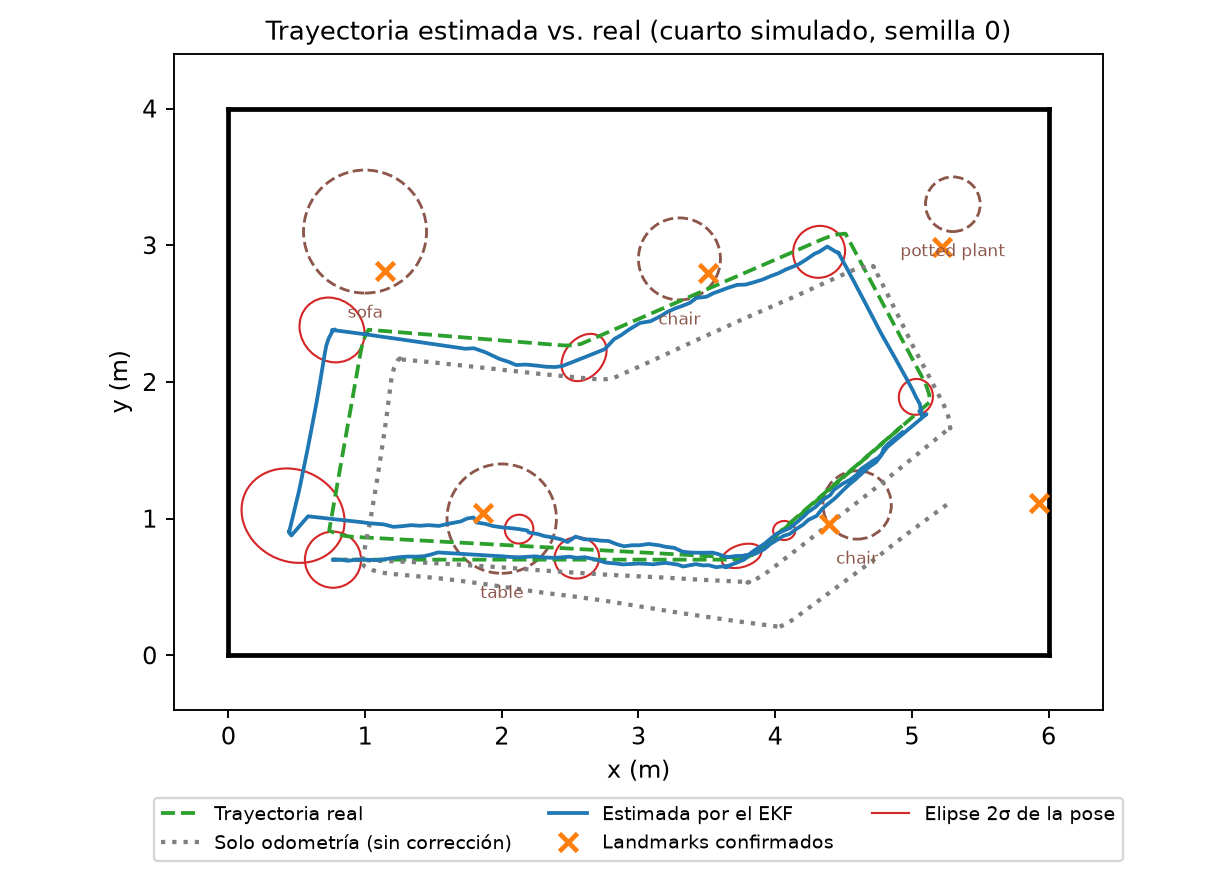
\includegraphics[width=0.85\textwidth]{Capturas_TT2/slam_trayectorias.png}
    \caption{Trayectoria real, estimada por el EKF y solo con odometría en el cuarto
    simulado. Los círculos discontinuos son los obstáculos reales.}
    \label{fig:slam_trayectorias}
\end{figure}

La Tabla~\ref{tab:slam_semillas} reporta seis corridas con semillas aleatorias
distintas.

\begin{table}[H]
\centering
\caption{Resultados del SLAM en el banco de simulación (300 ciclos por corrida)}
\label{tab:slam_semillas}
\renewcommand{\arraystretch}{1.2}
\begin{tabular}{|c|c|c|c|c|}
\hline
\textbf{Semilla} & \textbf{ATE EKF (m)} & \textbf{ATE solo odometría (m)} &
\textbf{Error de orientación} & \textbf{Landmarks} \\
\hline
0 & 0.142 & 0.318 & $2.31^\circ$ & 6 \\
1 & 0.288 & 0.250 & $4.16^\circ$ & 7 \\
2 & 0.270 & 0.273 & $3.86^\circ$ & 6 \\
3 & 0.116 & 0.191 & $2.64^\circ$ & 7 \\
4 & 0.249 & 0.164 & $1.71^\circ$ & 6 \\
5 & 0.205 & 0.188 & $2.48^\circ$ & 8 \\
\hline
\textbf{Promedio} & \textbf{0.212} & \textbf{0.231} & $\mathbf{2.86^\circ}$ & \textbf{6.7} \\
\hline
\end{tabular}
\end{table}

Estos números hay que leerlos con cuidado. En promedio el EKF baja el error de 0.23 a
0.21~m, pero no en todas las corridas, porque en dos de las seis la odometría sola fue
más precisa. En recorridos cortos y sin sesgo, como los del banco, integrar la odometría
ya da un buen resultado, y las correcciones contra \emph{landmarks} ubicados con
distancia monocular meten un error parecido al que quitan. Con una odometría real la
historia cambia, porque la longitud de paso nunca queda perfectamente calibrada y los
sensores tienen sesgo. Para ver ese caso se repitió el experimento con recorridos de
1200 ciclos (unas cuatro vueltas al cuarto) y con odometría sesgada; los resultados están
en la Tabla~\ref{tab:slam_deriva} y en la Figura~\ref{fig:slam_deriva}.

\begin{table}[H]
\centering
\caption{ATE promedio (y máximo) en seis corridas con odometría sesgada}
\label{tab:slam_deriva}
\renewcommand{\arraystretch}{1.2}
\begin{tabular}{|p{5.6cm}|c|c|}
\hline
\textbf{Escenario} & \textbf{EKF (m)} & \textbf{Solo odometría (m)} \\
\hline
300 ciclos, sin sesgo & 0.21 (0.29) & 0.23 (0.32) \\
1200 ciclos, sin sesgo & 0.28 (0.35) & 0.42 (0.61) \\
1200 ciclos, longitud de paso +10\,\% & 0.38 (0.62) & 0.58 (0.80) \\
1200 ciclos, giro sesgado $+0.1^\circ$/ciclo & 0.89 (1.68) & 1.64 (1.86) \\
1200 ciclos, ambos sesgos & 1.34 (1.89) & 1.75 (2.01) \\
\hline
\end{tabular}
\end{table}

\begin{figure}[H]
    \centering
    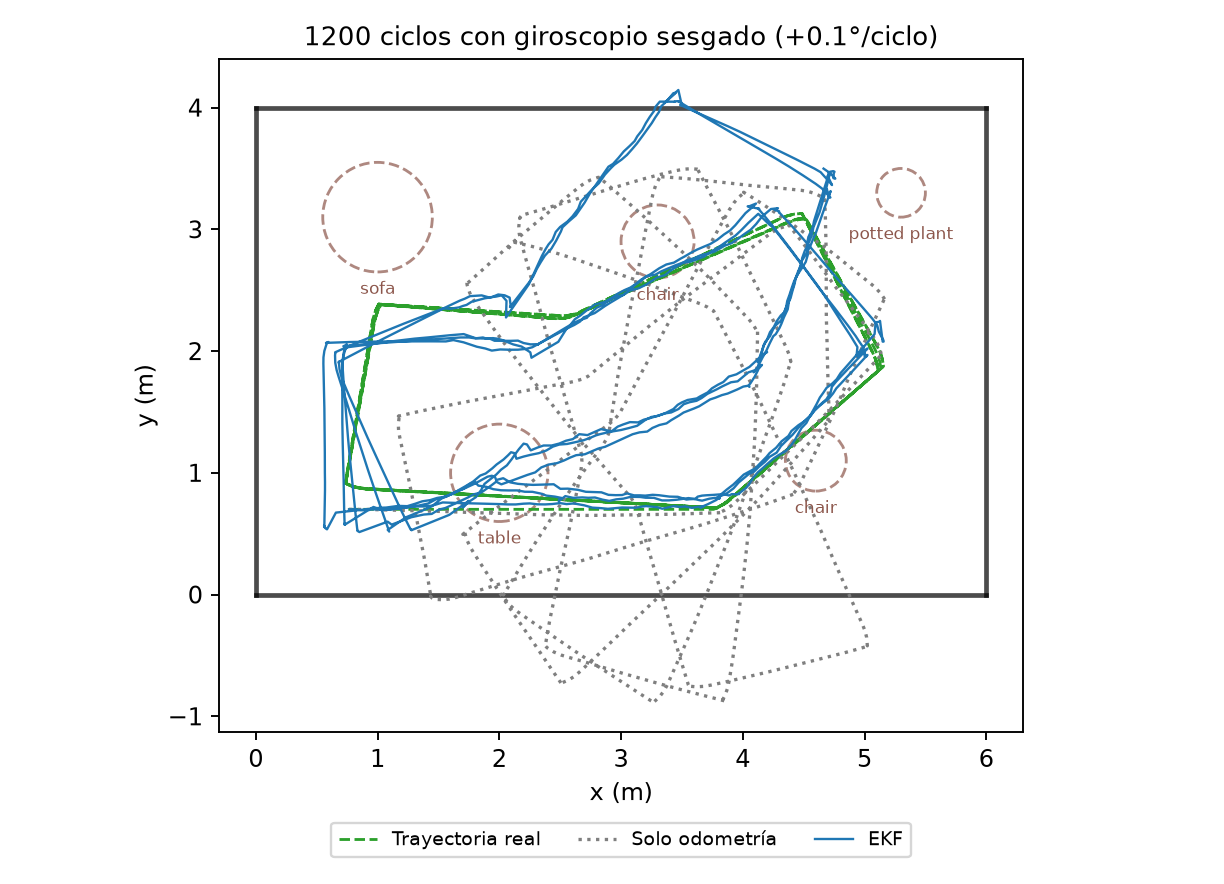
\includegraphics[width=0.78\textwidth]{Capturas_TT2/slam_deriva.png}
    \caption{Recorrido de 1200 ciclos con giroscopio sesgado (semilla 0). La odometría
    sola va girando el recorrido; el EKF lo mantiene cerca del real, aunque con
    desviaciones de hasta un metro en algunos tramos.}
    \label{fig:slam_deriva}
\end{figure}

En recorridos largos y con error de escala en el paso, el EKF reduce el error de la
odometría en alrededor de un tercio, que es justo para lo que sirve el SLAM. Con el
giroscopio sesgado lo reduce casi a la mitad en promedio, aunque el máximo llega a
1.7~m, y con los dos sesgos juntos la mejora baja a una cuarta parte. En esas corridas
se observó una divergencia de orientación, ya que en dos de las seis el error de rumbo
pasó de $100^\circ$ hacia el final. Con el rumbo tan equivocado, las detecciones dejan
de asociarse con los \emph{landmarks} que ya existen y se crean duplicados desplazados
(hasta diez sillas en un cuarto que tiene dos), y el filtro termina siendo consistente
con un mapa erróneo. Es la forma típica en que falla un EKF sin cierre de lazo.

En el prototipo este caso es poco probable, porque el giro no se integra a partir del
giroscopio sino que se toma del rumbo que entrega la BNO055 en su modo de fusión con
magnetómetro. Ese rumbo es absoluto, así que el sesgo no se va sumando como en la
simulación. Para que funcione, la brújula debe estar calibrada; por eso, al arrancar,
el sistema revisa el estado de calibración del magnetómetro y, si es bajo, le pide al
usuario que mueva los lentes en forma de ocho. El experimento sigue siendo útil por dos
razones, ya que muestra lo que pasaría con una brújula mal calibrada o alterada por
estructuras metálicas, y describe el modo de respaldo sin IMU, en el que el giro sale
del flujo óptico y sí acumula error.

\textbf{Pérdida de observaciones.} Para probar el manejo de oclusiones se repitió la
corrida de la semilla 0 quitando todas las detecciones visuales entre los ciclos 120 y
200. En la Figura~\ref{fig:slam_incertidumbre} se ve que, durante la oclusión, la traza
de la covarianza crece sin parar y la confianza cae casi a cero, es decir, el sistema se
da cuenta de que su pose ya no es fiable. En cuanto vuelve a ver objetos conocidos
(ciclo 220), la incertidumbre se reduce de golpe. El ATE de esta corrida fue de
0.08~m, así que la oclusión no hizo que el sistema se perdiera. En la corrida normal
también hay caídas de confianza en los tramos donde la cámara no tiene objetos a la
vista.

\begin{figure}[H]
    \centering
    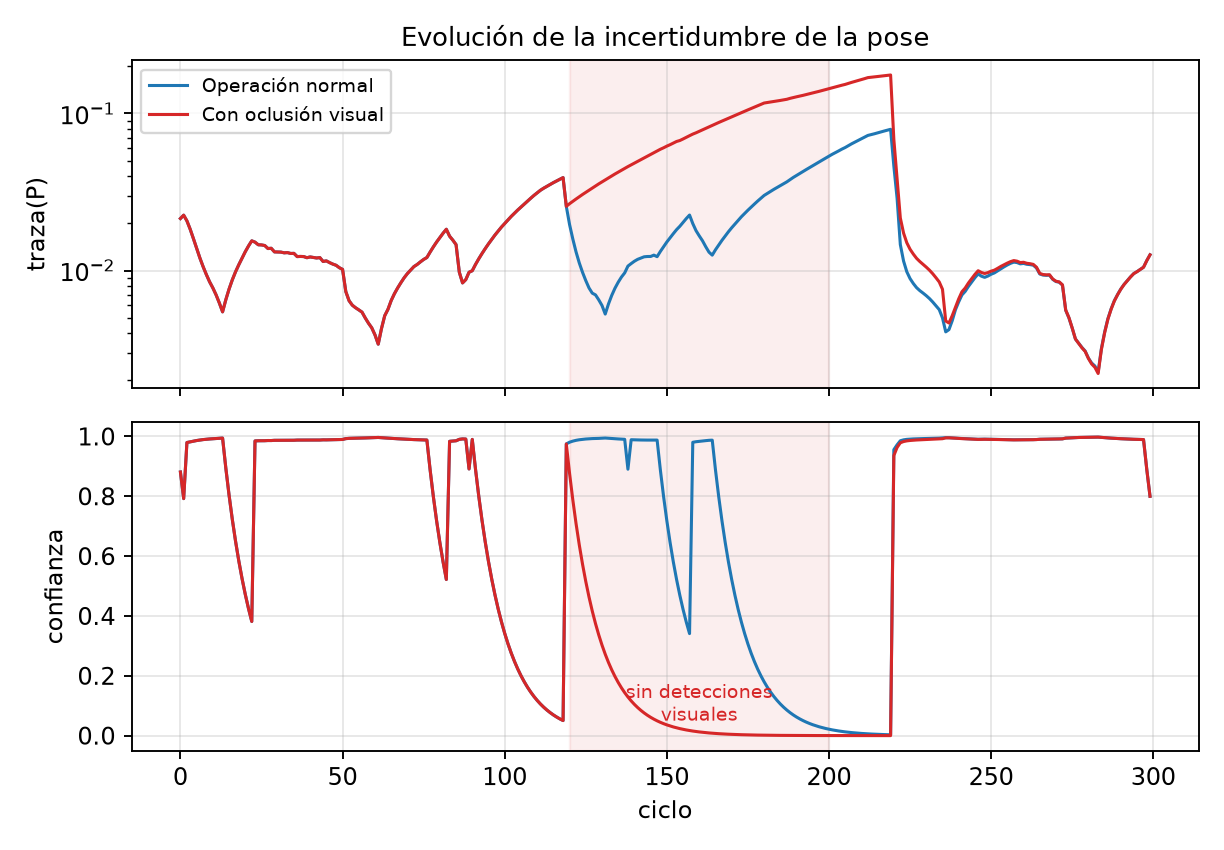
\includegraphics[width=0.85\textwidth]{Capturas_TT2/slam_incertidumbre.png}
    \caption{Evolución de la traza de la covarianza (escala logarítmica) y de la
    confianza, con y sin oclusión visual entre los ciclos 120 y 200.}
    \label{fig:slam_incertidumbre}
\end{figure}

Al quitar al azar el 60\,\% de las detecciones visuales en las seis corridas, el ATE
promedio fue de 0.23~m (máximo 0.28~m), por lo que el módulo aguanta bien las
detecciones intermitentes.

\textbf{Videos reales.} En los 19 videos grabados, el SLAM confirmó entre 1 y 39
\emph{landmarks} por recorrido. En interiores la clase más frecuente fue la puerta,
con entre 9 y 17 por recorrido de oficina. En las calles hubo muy pocos objetos
estáticos de las clases que se detectan, y en el recorrido más pobre se confirmó uno
solo, de modo que el sistema avanzó casi todo el tiempo con la pura predicción. La
Sección~\ref{sec:dev_integracion} presenta capturas del sistema trabajando con video.

\textbf{Costo computacional.} Un ciclo del EKF tarda en promedio 0.03~ms en el banco,
con unos siete \emph{landmarks}, y 0.27~ms con video real, con unos cuarenta, porque la
asociación crece linealmente con su número. En la Raspberry Pi del prototipo el ciclo
tarda \TODO{tiempo por ciclo del EKF en la Raspberry Pi}. En cualquier caso el costo es
mínimo frente a los 100~ms por ciclo que permite RNF-03.

\subsection{Limitaciones}

El rumbo absoluto de la BNO055 depende de que el magnetómetro esté calibrado y de que no
haya perturbaciones magnéticas cerca, como estructuras de acero o equipos eléctricos. La
calibración se revisa al arrancar, pero durante la sesión ningún módulo reacciona si
empeora. \TODO{avisar al usuario si la calibración del magnetómetro baja durante la
sesión}.

El filtro no hace cierre de lazo (\emph{loop closure}). Si la deriva es grande al
regresar a una zona ya visitada, el error no se reparte a lo largo de la trayectoria
anterior, y si el error de orientación rebasa lo que tolera la compuerta de asociación,
aparecen \emph{landmarks} duplicados y el filtro puede divergir. La posición de los
\emph{landmarks} monoculares depende además de la altura típica de su clase, así que un
objeto de tamaño poco común puede quedar mal ubicado, como el que aparece junto a la
pared en la Figura~\ref{fig:slam_trayectorias}. La asociación por vecino más cercano
también puede confundir dos objetos cercanos de la misma clase; una prueba de
compatibilidad conjunta \cite{neira2001jcbb} sería más confiable, a cambio de más
cómputo.

Por último, los valores de ruido de la odometría se ajustaron en simulación.
\TODO{medir el ruido real de la IMU y del conteo de pasos en el prototipo y actualizar
los parámetros del filtro}. En los mapas que se obtienen de video la escala depende de
la velocidad de caminata supuesta, porque el video no trae información de
desplazamiento.


% ==============================================================================
\section{Módulo de Ray Casting}
\label{sec:dev_ray}
% ==============================================================================

\subsection{Descripción}

El módulo de Ray Casting, implementado en \texttt{occupancy\_grid.py}, es el puente
entre las observaciones del SLAM y el mapa de ocupación. En el sistema final cumple
dos funciones distintas que comparten el mismo núcleo de recorrido de celdas:

\begin{enumerate}
    \item \textbf{Actualización del mapa.} Desde la pose estimada se traza un rayo por
    cada observación; las celdas atravesadas acumulan evidencia de espacio libre y la
    celda del extremo acumula evidencia de ocupación. Esto corresponde al modelo
    inverso del sensor de los mapas de ocupación \cite{moravec1985sonar, elfes1989}.
    \item \textbf{Consulta del mapa.} Desde la pose actual se lanzan rayos virtuales
    sobre el mapa ya construido para medir la distancia libre en cada dirección. Estas
    distancias son las variables $d_{\text{front}}$, $d_{\text{left}}$ y
    $d_{\text{right}}$ que recibe el módulo de navegación.
\end{enumerate}

En el diseño de TT1 solo se contemplaba la primera función con la regla básica ``libre
en el recorrido, ocupado al final''. Durante el desarrollo esa regla resultó
insuficiente porque las observaciones del sistema tienen precisiones muy distintas
(5~cm del ultrasonido frente a $\pm 30$\,\% de la estimación monocular), por lo que se
añadieron las reglas descritas en esta sección.

\subsection{Discretización y recorrido de celdas}

El plano se discretiza en celdas de $5 \times 5$~cm. Un punto $(x, y)$ del mundo
corresponde a la celda $(\lfloor x / 0.05 \rfloor,\; \lfloor y / 0.05 \rfloor)$, y el
extremo de un rayo con rango $r$ y dirección relativa $\phi$ desde la pose
$(x, y, \theta)$ es:

\[
x_e = x + r\cos(\theta + \phi),
\qquad
y_e = y + r\sin(\theta + \phi)
\]

Las celdas atravesadas entre la celda del usuario y la del extremo se obtienen con el
algoritmo de Bresenham \cite{bresenham1965}, que avanza celda por celda utilizando
únicamente sumas y comparaciones de enteros (Figura~\ref{fig:ray_bresenham}). Para un
alcance máximo de 4~m, un rayo recorre a lo sumo 80 celdas. Se consideró el algoritmo
de recorrido de vóxeles de Amanatides y Woo \cite{amanatides1987voxel}, que visita
todas las celdas que toca el segmento, pero Bresenham resultó suficiente para la
actualización y es más sencillo; la consecuencia de esta elección en la consulta se
discute en las limitaciones.

\begin{figure}[H]
    \centering
    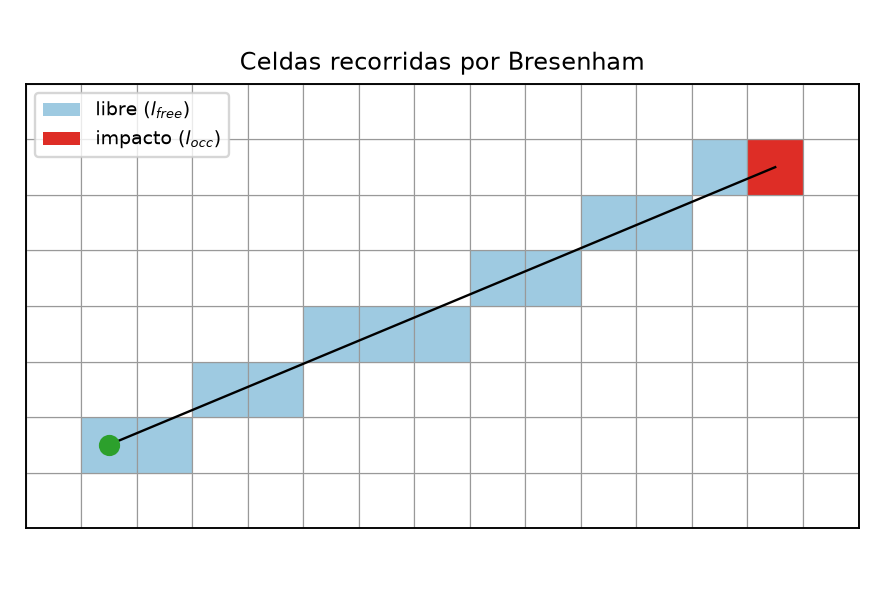
\includegraphics[width=0.6\textwidth]{Capturas_TT2/raycasting_bresenham.png}
    \caption{Celdas recorridas por el algoritmo de Bresenham para un rayo: las celdas
    intermedias reciben evidencia de espacio libre y la celda del extremo, de
    ocupación.}
    \label{fig:ray_bresenham}
\end{figure}

\subsection{Modelo inverso del sensor en log-odds}

Cada celda almacena el logaritmo de la razón de probabilidades de estar ocupada,
$l = \log\frac{p}{1-p}$, de modo que la fusión de una nueva observación es una suma
\cite{thrun2005probabilistic}. La probabilidad se recupera como
$p = 1/(1 + e^{-l})$. La Tabla~\ref{tab:ray_constantes} resume las constantes
utilizadas.

\begin{table}[H]
\centering
\caption{Constantes del modelo inverso del sensor}
\label{tab:ray_constantes}
\renewcommand{\arraystretch}{1.25}
\begin{tabular}{|p{2.6cm}|c|c|p{6.8cm}|}
\hline
\textbf{Constante} & \textbf{Log-odds} & \textbf{Probabilidad} & \textbf{Significado} \\
\hline
$l_{occ}$ & $+1.2$ & 0.77 & Incremento en la celda donde termina un rayo preciso. \\
\hline
$l_{free}$ & $-0.4$ & 0.40 & Incremento en cada celda atravesada. \\
\hline
$l_{\min}, l_{\max}$ & $\pm 5.0$ & 0.007 / 0.993 & Saturación de la celda. \\
\hline
Umbral de ocupado & $1.0$ & 0.73 & Por encima, la celda se considera obstáculo. \\
\hline
$L_{block}$ & $2.0$ & 0.88 & Por encima, la celda se considera una superficie
consolidada que detiene los rayos de espacio libre. \\
\hline
\end{tabular}
\end{table}

La asimetría entre $l_{occ}$ y $l_{free}$ es intencional: un rayo atraviesa muchas
celdas pero termina en una sola, por lo que la evidencia de ocupación debe pesar más
para que los obstáculos no se borren por los rayos que pasan junto a ellos. La
saturación en $\pm 5$ evita que una celda acumule tanta evidencia que después no pueda
corregirse \cite{hornung2013octomap}. La Figura~\ref{fig:ray_logodds} muestra el
efecto con las mismas reglas del código: una celda que se vio libre muchas veces
necesita seis impactos para volver a considerarse ocupada cuando aparece un
obstáculo. La figura también muestra la limitación discutida al final de esta
sección: una vez que la celda supera $L_{block}$, los rayos de espacio libre se
detienen en ella y su valor ya no disminuye aunque el obstáculo se retire.

\begin{figure}[H]
    \centering
    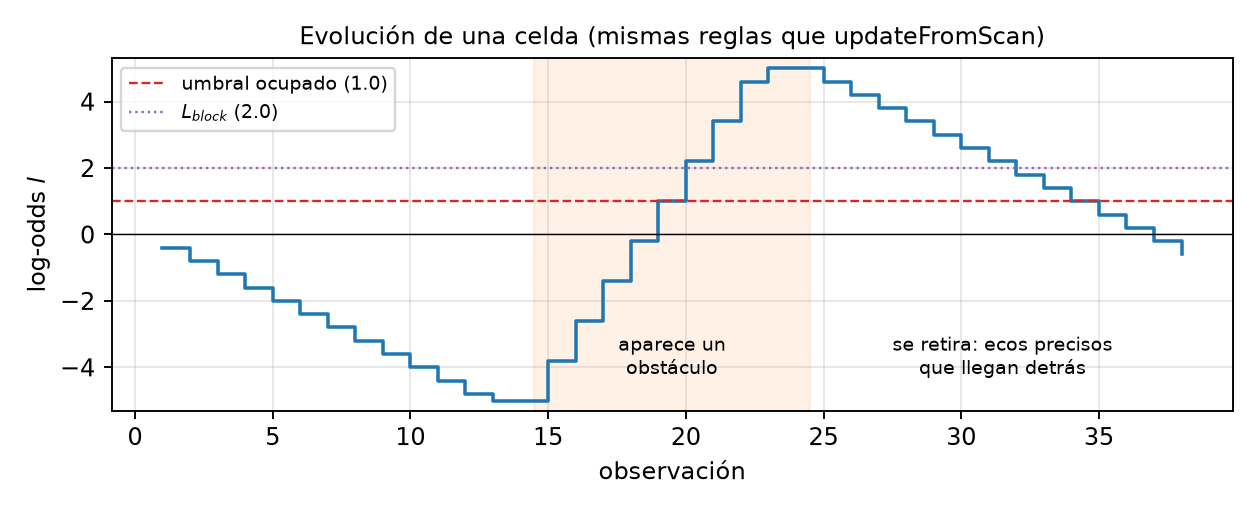
\includegraphics[width=0.82\textwidth]{Capturas_TT2/raycasting_logodds.png}
    \caption{Evolución del log-odds de una celda que primero se observa libre, después
    ocupada y finalmente queda libre otra vez, calculada con las reglas de
    \texttt{updateFromScan}.}
    \label{fig:ray_logodds}
\end{figure}

\subsection{Reglas añadidas durante el desarrollo}

Sobre el modelo básico se implementaron las siguientes reglas, cada una motivada por
un problema observado durante las pruebas:

\begin{enumerate}
    \item \textbf{El rango impreciso no marca ocupación.} Si la observación tiene
    $\sigma_r > 0.15$~m (estimación monocular cruda), el rayo solo despeja espacio
    libre hasta $r - 2\sigma_r$ y no marca la celda final como ocupada. El propósito
    es evitar que el ruido monocular deje manchas de celdas ocupadas alrededor de cada
    objeto y que despeje como libre el espacio donde realmente está el objeto. La
    ocupación de los objetos detectados por visión llega al mapa por la vía precisa:
    el rayo anclado a la posición consolidada del \emph{landmark} que genera el SLAM.
    \item \textbf{Las superficies consolidadas detienen el rayo.} Si al recorrer el
    rayo se encuentra una celda con $l > L_{block}$, el recorrido se detiene y no se
    marca nada más allá. Así un rayo ruidoso no perfora una pared ya registrada ni
    pinta marcas fantasma detrás de ella.
    \item \textbf{Rayos sin eco.} Cuando un sensor ultrasónico no recibe eco, se genera
    un rayo de espacio libre con la longitud del alcance máximo; como su extremo cae
    fuera del alcance útil, no marca ocupación. Esto permite registrar pasillos libres.
    \item \textbf{Recorte en lugar de descarte.} En la retícula de tamaño fijo, si el
    extremo de un rayo cae fuera del mapa, el rayo se recorta en el borde y se
    conservan las celdas libres recorridas. Inicialmente esos rayos se descartaban
    completos. En el mapa por bloques (Sección~\ref{sec:dev_mapeo}) esta regla deja de
    ser necesaria porque el mapa no tiene bordes.
    \item \textbf{Alcance máximo.} Los rayos se limitan a 4~m; una observación más
    lejana solo despeja espacio libre hasta ese límite.
    \item \textbf{Peligros de piso.} Las observaciones marcadas como peligro (hoyos,
    agua, escaleras) no modifican el log-odds, ya que el espacio por encima de un hoyo
    está libre; en su lugar suman un impacto en una capa separada que se describe en
    el módulo de mapeo.
\end{enumerate}

La Figura~\ref{fig:ray_casos} muestra el resultado de ejecutar el código del módulo en
tres casos representativos, con celdas de 10~cm para facilitar su lectura.

\begin{figure}[H]
    \centering
    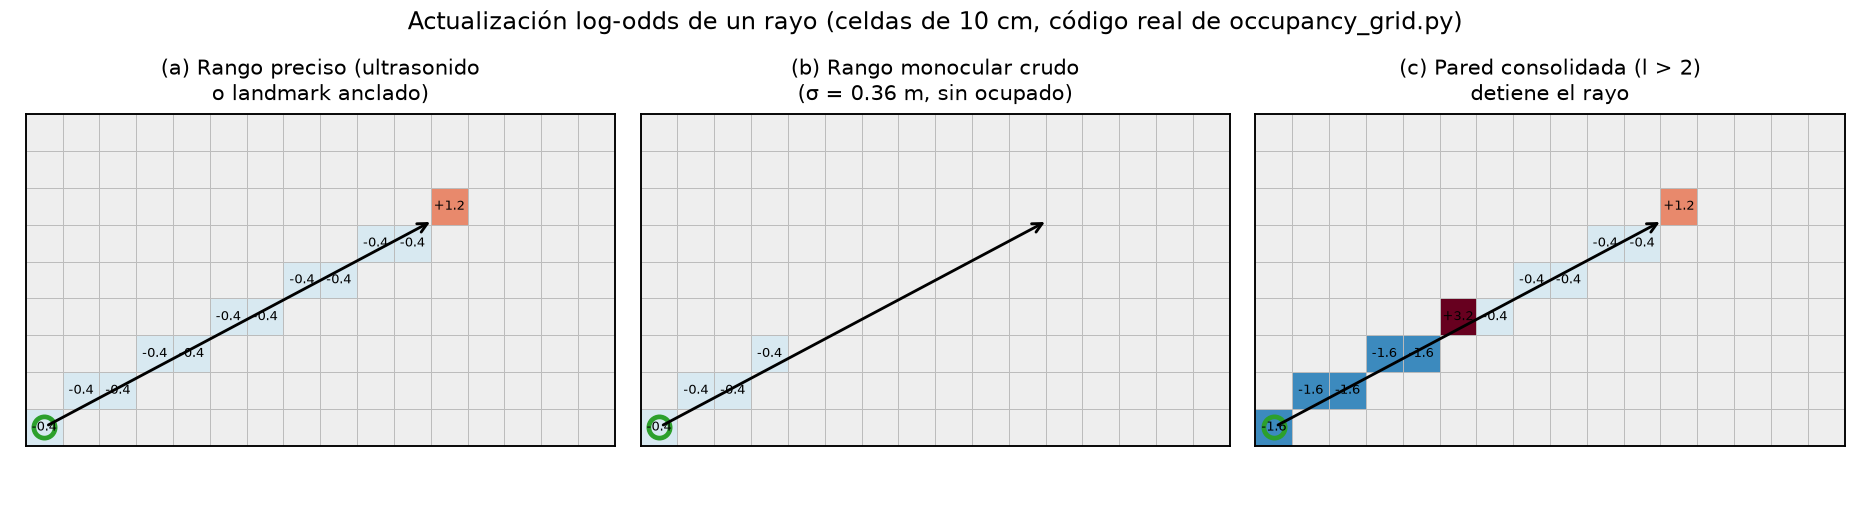
\includegraphics[width=\textwidth]{Capturas_TT2/raycasting_casos.png}
    \caption{Actualización de un rayo en tres casos: (a) rango preciso, que despeja el
    recorrido y marca el extremo; (b) rango monocular crudo, que solo despeja hasta
    $r - 2\sigma_r$; (c) rayo detenido por una superficie consolidada.}
    \label{fig:ray_casos}
\end{figure}

El Algoritmo~\ref{alg:dev_ray_update} describe la actualización tal como quedó
implementada en \texttt{updateFromScan}.

\begin{center}
\captionof{algorithm}{Actualización del mapa por Ray Casting}
\label{alg:dev_ray_update}
\end{center}
\vspace{-1.8cm}
\rule{\textwidth}{0.4pt}
\vspace{-0.9cm}
\begin{algorithmic}[1]

\Statex \textbf{ENTRADA:}
\Statex pose \Comment{(x, y, $\theta$) estimada por el SLAM}
\Statex observaciones \Comment{ancladas a landmarks + ecos + rayos sin eco}
\Statex alcance\_max \Comment{4 m}
\Statex \textbf{SALIDA:}
\Statex mapa actualizado (log-odds y capa de peligros)

\Statex
\State celda\_origen $\gets$ a\_celda(x, y)
\For{cada obs en observaciones}
    \State r $\gets$ mín(obs.r, alcance\_max)
    \State impreciso $\gets$ obs.$\sigma_r > 0.15$
    \State extremo $\gets$ a\_celda(x + r cos($\theta$ + obs.$\phi$), y + r sin($\theta$ + obs.$\phi$))
    \State celdas $\gets$ bresenham(celda\_origen, extremo)
    \State libres $\gets$ celdas sin la última
    \If{impreciso}
        \State libres $\gets$ primeras celdas hasta la distancia r $- 2\sigma_r$
    \EndIf
    \State bloqueado $\gets$ falso
    \For{cada c en libres}
        \If{l(c) $> L_{block}$}
            \State bloqueado $\gets$ verdadero;\; salir del ciclo
        \EndIf
        \State l(c) $\gets$ saturar(l(c) + $l_{free}$, $-5$, $+5$)
    \EndFor
    \If{no bloqueado Y obs.r $\leq$ alcance\_max}
        \If{obs es peligro de piso}
            \State peligros(extremo) $\gets$ mín(peligros(extremo) + 1, 10)
        \ElsIf{no impreciso}
            \State l(extremo) $\gets$ saturar(l(extremo) + $l_{occ}$, $-5$, $+5$)
        \EndIf
    \EndIf
\EndFor

\end{algorithmic}
\vspace{-0.9cm}
\rule{\textwidth}{0.4pt}

\subsection{Rayos de consulta}

La segunda función del módulo es medir el espacio libre alrededor del usuario sobre
el mapa construido. La función \texttt{castDistance} recorre con Bresenham las celdas
desde la pose en una dirección dada y devuelve la distancia al centro de la primera
celda bloqueada, entendida como una celda con $l > 1.0$ o con al menos dos impactos
en la capa de peligros; si no encuentra ninguna, devuelve el alcance máximo de 4~m.

Para construir las variables del vector de estado del módulo de navegación, la
función \texttt{directionDistances} divide el entorno del usuario en tres sectores
(Figura~\ref{fig:ray_sectores}): frente ($|\phi| \leq 30^\circ$), izquierda
($30^\circ < \phi \leq 90^\circ$) y derecha ($-90^\circ \leq \phi < -30^\circ$). En
cada sector se lanzan cinco rayos equiespaciados y se conserva la distancia mínima,
lo cual es conservador: basta con que un rayo encuentre un obstáculo para que el
sector se considere ocupado a esa distancia.

\begin{figure}[H]
    \centering
    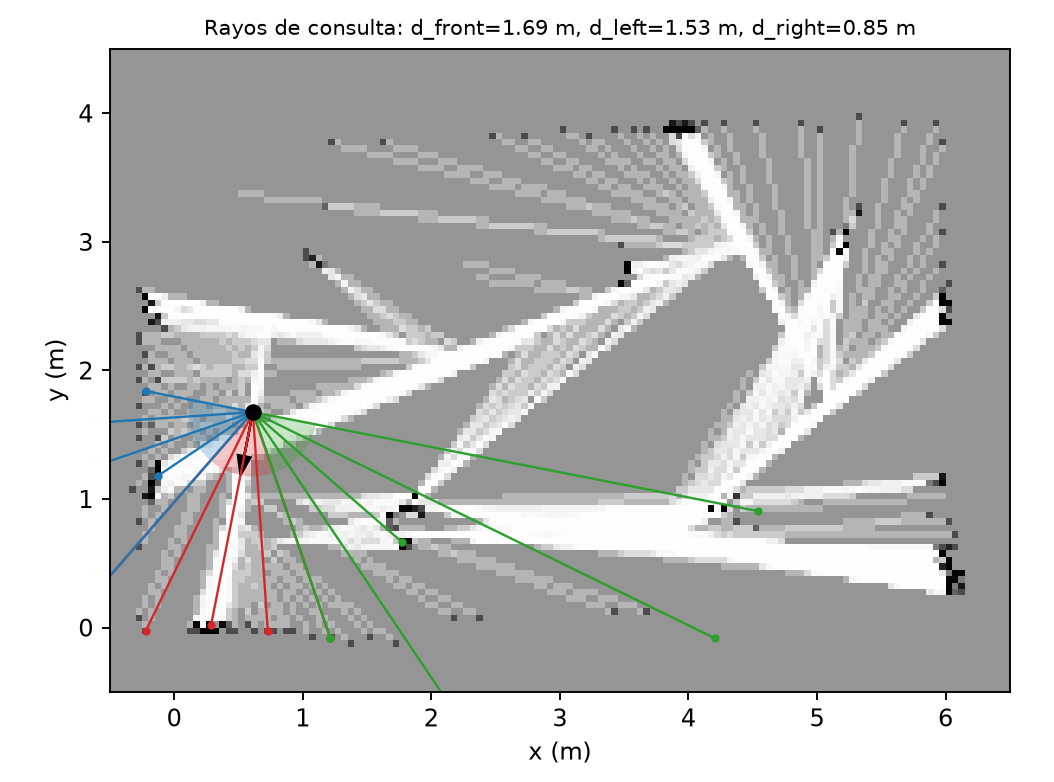
\includegraphics[width=0.75\textwidth]{Capturas_TT2/raycasting_sectores.png}
    \caption{Rayos de consulta por sector sobre el mapa construido en simulación. El
    título indica las distancias resultantes que se entregan al módulo de
    navegación.}
    \label{fig:ray_sectores}
\end{figure}

\begin{center}
\captionof{algorithm}{Distancias libres por sector}
\label{alg:dev_ray_query}
\end{center}
\vspace{-1.8cm}
\rule{\textwidth}{0.4pt}
\vspace{-0.9cm}
\begin{algorithmic}[1]

\Statex \textbf{ENTRADA:} mapa, pose (x, y, $\theta$), alcance\_max = 4 m
\Statex \textbf{SALIDA:} $d_{\text{front}}$, $d_{\text{left}}$, $d_{\text{right}}$

\Statex
\Function{castDistance}{x, y, $\alpha$}
    \For{cada c en bresenham(a\_celda(x, y), a\_celda(x + 4 cos $\alpha$, y + 4 sin $\alpha$))}
        \If{c no es la celda del usuario Y (l(c) $> 1.0$ O peligros(c) $\geq 2$)}
            \State \Return mín(4, distancia(x, y, centro(c)))
        \EndIf
    \EndFor
    \State \Return 4
\EndFunction

\Statex
\For{cada sector (a0, a1) en \{frente: ($-30^\circ$, $30^\circ$), izq: ($30^\circ$, $90^\circ$), der: ($-90^\circ$, $-30^\circ$)\}}
    \State d $\gets$ 4
    \For{k = 0 hasta 4}
        \State d $\gets$ mín(d, castDistance(x, y, $\theta$ + a0 + (a1 $-$ a0) k / 4))
    \EndFor
    \State d\_sector $\gets$ d
\EndFor
\State \Return $d_{\text{front}}$, $d_{\text{left}}$, $d_{\text{right}}$

\end{algorithmic}
\vspace{-0.9cm}
\rule{\textwidth}{0.4pt}

El módulo de navegación utiliza además una versión vectorizada con NumPy del mismo
principio para simular sensores durante el entrenamiento del agente, la cual se
documentará junto con ese módulo.

\subsection{Resultados}

En el banco de simulación, la actualización del mapa con todas las observaciones de un
ciclo (cuatro a seis rayos) tomó en promedio 0.15~ms, y en el procesamiento de video
real, incluyendo el despeje de la huella del usuario, 0.23~ms por ciclo. La
construcción completa del cuadro para navegación, que incluye los quince rayos de
consulta y el mapa local, tomó 0.51~ms. Estos tiempos son dos órdenes de magnitud
menores que el periodo de 100~ms que impone RNF-03, por lo que el Ray Casting no
representa un cuello de botella del sistema.

Para cuantificar la aportación de las reglas añadidas se realizó un experimento de
ablación en el banco de simulación, desactivándolas una por una. Además de la
precisión y la exhaustividad, se contó el número de celdas marcadas como ocupadas que
no tienen ningún obstáculo real a menos de 10~cm (celdas falsas). Los resultados se
muestran en la Tabla~\ref{tab:ray_ablacion}.

\begin{table}[H]
\centering
\caption{Ablación de las reglas del Ray Casting (promedio de seis corridas)}
\label{tab:ray_ablacion}
\renewcommand{\arraystretch}{1.2}
\begin{tabular}{|p{6.0cm}|c|c|c|c|}
\hline
\textbf{Configuración} & \textbf{Precisión} & \textbf{Exhaustividad} &
\textbf{Ocupadas} & \textbf{Falsas} \\
\hline
Vigente (todas las reglas) & 0.60 & 0.31 & 152 & 60 \\
Sin $L_{block}$ & 0.58 & 0.30 & 172 & 73 \\
Rango monocular crudo marca ocupación & 0.60 & 0.32 & 157 & 63 \\
Sin anclar a \emph{landmarks} (rango crudo) & 0.62 & 0.31 & 150 & 57 \\
Sin las tres reglas & 0.57 & 0.35 & 192 & 82 \\
\hline
\end{tabular}
\end{table}

En conjunto, las reglas reducen las celdas falsas de 82 a 60 (alrededor de 27\,\%), y
la mayor parte de esa mejora proviene de $L_{block}$. Quitar las tres reglas sube un
poco la exhaustividad, porque el mapa marca más celdas, pero a costa de más celdas
falsas. Las reglas del rango monocular y del anclaje casi no modifican las métricas
globales del banco, porque la mayoría de las celdas ocupadas corresponden a paredes
registradas por ultrasonido y los objetos son una fracción pequeña del mapa; su
efecto es local, alrededor de cada objeto, donde evitan manchas difusas y marcas
duplicadas. También se observa que cerca del 40\,\% de las celdas ocupadas no
coinciden con un obstáculo real dentro de la tolerancia de 10~cm. La causa principal
no es el Ray Casting sino el error de pose: con un ATE de 0.21~m, una pared registrada
en distintos momentos queda dibujada con un desplazamiento de varias celdas. La Sección~\ref{sec:dev_mapeo}
analiza la calidad del mapa con mayor detalle.

\subsection{Limitaciones}

\begin{itemize}
    \item \textbf{Celdas consolidadas permanentes.} La regla $L_{block}$ impide que un
    rayo de espacio libre atraviese una celda con $l > 2$, lo cual también impide que
    esa celda vuelva a disminuir. En la práctica, una celda que recibió dos o más
    impactos precisos queda marcada como ocupada de forma permanente: se verificó que
    ni cincuenta rayos posteriores que la atraviesan la liberan. Esto significa que
    un obstáculo que desaparece (por ejemplo, una caja que se retira) permanece en el
    mapa, lo cual no cumple por completo con RF-17 en el caso de desaparición de
    obstáculos. Una corrección posible es permitir que los rayos precisos, cuyo
    extremo está claramente más allá de la celda, sí reduzcan su valor.
    \item \textbf{Huecos entre celdas.} Bresenham visita una sola celda por paso, por
    lo que un rayo de consulta diagonal puede pasar entre dos celdas ocupadas que solo
    se tocan por una esquina y reportar libre un frente bloqueado. Esto es frecuente en
    mapas con ecos dispersos. El módulo de navegación lo mitiga lanzando un abanico de
    tres sub-rayos por dirección; una alternativa sería usar el recorrido de
    Amanatides y Woo en la consulta.
    \item \textbf{Mapa bidimensional.} Los rayos se trazan en el plano, por lo que
    obstáculos colgantes (ramas, letreros a la altura de la cabeza) solo se registran
    si los detecta la visión.
    \item Como el rango monocular nunca marca ocupación por sí solo, los obstáculos de
    clases que la visión no reconoce y que no producen eco ultrasónico no aparecen en
    el mapa.
\end{itemize}


% ==============================================================================
\section{Módulo de mapeo}
\label{sec:dev_mapeo}
% ==============================================================================

\subsection{Descripción}

El módulo de mapeo mantiene la representación del entorno sobre la que trabajan la
navegación y las alertas, y atiende los requerimientos RF-15, RF-16 y RF-17. El diseño
de TT1 contemplaba una sola retícula de ocupación local. La primera implementación
(\texttt{occupancy\_grid.py}) siguió ese diseño con una retícula fija de
$8 \times 8$~m, pero pronto aparecieron tres problemas. El usuario puede salir de un
área de ocho metros en pocos segundos; una retícula más grande gastaría memoria aunque
casi toda quedara vacía; y el mapa se perdía al apagar el dispositivo. Para resolverlos
se desarrolló el gestor de mapa por bloques (\texttt{map\_manager.py}), que conserva la
misma interfaz de consulta de la retícula original, así que el resto del sistema no tuvo
que cambiar.

\subsection{Mapa global por bloques}

El plano se divide en bloques cuadrados fijos (\emph{chunks}) de $8 \times 8$~m,
anclados al marco de referencia del SLAM. Con celdas de 5~cm, cada bloque tiene
$160 \times 160$ celdas. Los bloques se identifican con un par de índices enteros
$(i, j)$, que pueden ser negativos, y se crean solo cuando un rayo o el propio usuario
llegan a ellos, de modo que el mapa crece únicamente hacia donde se camina. Un punto del
mundo se convierte a su bloque y a su celda local así.

\[
(g_x, g_y) = \left(\left\lfloor \frac{x}{0.05} \right\rfloor,
                   \left\lfloor \frac{y}{0.05} \right\rfloor\right),
\qquad
(i, j) = \left(\left\lfloor \frac{g_x}{160} \right\rfloor,
               \left\lfloor \frac{g_y}{160} \right\rfloor\right),
\qquad
(l_x, l_y) = (g_x - 160\,i,\; g_y - 160\,j)
\]

La idea se parece a los submapas de sistemas como Cartographer
\cite{hess2016cartographer}, con la diferencia de que aquí los bloques tienen una
posición fija en el mundo y no se reacomodan por optimización. Eso mantiene el costo
bajo, a cambio de no corregir la deriva acumulada.

Cada bloque (\texttt{MapChunk}) guarda una matriz de log-odds en punto flotante de
32 bits, que ocupa 100~KB en memoria, y una matriz de impactos de peligros de piso en
enteros de 8 bits, de 25~KB. Guarda también la etiqueta del cuarto al que pertenece, el
número de visitas, las fechas de creación y de última visita, y una bandera que indica
si tiene cambios sin guardar.

Para no llenar la memoria de la Raspberry Pi, se mantienen como máximo 25 bloques
cargados. Si se pasa de ese número, los bloques más alejados del actual (en distancia de
Chebyshev) se guardan en disco y se descargan, y si se vuelven a necesitar se cargan de
nuevo sin que el resto del sistema lo note. Los rayos cruzan de un bloque a otro sin
cortes, porque cada celda se resuelve a su bloque en el momento de leerla o escribirla,
con un pequeño caché del último bloque consultado.

\subsection{Persistencia y re-localización}

Cada mapa se guarda en una carpeta con la siguiente estructura.

\begin{verbatim}
maps/<nombre>/
    chunk_0_0.npz      log-odds (float16) + peligros + metadatos del bloque
    chunk_0_-1.npz     ...
    meta.json          resolución, tamaño de bloque, cuartos etiquetados
    landmarks.json     landmarks confirmados del SLAM (posición, etiqueta,
                       número de avistamientos)
\end{verbatim}

Los bloques se guardan comprimidos y con el log-odds en 16 bits, así que en los mapas
reales ocupan entre 1 y 7~KB cada uno y el recorrido más grande (13 bloques y
26 \emph{landmarks}) ocupa unos 60~KB. Al abrir un mapa se revisa que su resolución y
tamaño de bloque coincidan con la configuración actual, para no mezclar geometrías
distintas. Cuando el sistema arranca en un lugar ya mapeado, se restauran los bloques y
los \emph{landmarks}, y estos últimos se cargan en el SLAM para que el filtro pueda
corregir la pose contra objetos conocidos desde el primer ciclo.

El SLAM siempre arranca en el origen de su propio marco de referencia, así que la
re-localización funciona cuando el usuario empieza la sesión en el mismo punto y mirando
hacia el mismo lado que cuando se creó el mapa, por ejemplo en la entrada de su casa u
oficina. Una primera versión anunciaba como ``zona conocida'' cualquier bloque guardado
aunque el usuario estuviera en otro lugar. Ahora, mientras la re-localización está
pendiente, todos los bloques se reportan como nuevos y no se adoptan las etiquetas de
cuarto; se da por confirmada cuando el EKF acumula tres correcciones contra los
\emph{landmarks} cargados, y en ese momento el sistema lo dice en voz alta.

\subsection{Eventos de cambio de zona}

En cada ciclo el gestor recibe la pose y genera eventos que la interacción puede
anunciar por voz. El evento \texttt{chunk\_change} indica que el usuario entró a otro
bloque y si esa zona ya era conocida o es nueva. El evento \texttt{door\_crossed} se
dispara cuando el usuario pasa a menos de 0.7~m de un \emph{landmark} confirmado de tipo
puerta, lo cual se interpreta como el paso a otro cuarto, con una espera de 60 ciclos
para no repetirlo. Y \texttt{room\_recognized} indica que el bloque al que entró el
usuario tiene una etiqueta de cuarto guardada, como ``cocina''. Los cuartos se numeran
solos al cruzar puertas y se pueden renombrar con una etiqueta propia, que queda en
\texttt{meta.json}.

\subsection{Despeje de la huella del usuario}

Al procesar los videos se vio que, en pasillos sin objetos de las clases que reconoce la
visión, el mapa no registraba espacio libre, porque sin ultrasonido no había rayos que lo
despejaran, y la navegación no encontraba por dónde avanzar. Como el usuario sí pasó por
ahí, en cada ciclo se marca como libre un disco de 0.45~m de radio alrededor de su
posición (\texttt{clearFootprint}). Las celdas que ya superan el umbral de ocupación no
se tocan, para no borrar obstáculos reales.

\subsection{Capa de peligros de piso}

Un hoyo, una coladera, un charco o una escalera hacia abajo no devuelven eco ni detienen
un rayo, porque el espacio de arriba está libre, y aun así no se pueden pisar. Por eso
van en una capa separada del log-odds, siguiendo la idea de los mapas de costo por capas
\cite{lu2014layered}. Las detecciones vienen de la segmentación del módulo de visión
(SegFormer entrenado en ADE20K \cite{xie2021segformer, zhou2017ade20k}) y su distancia se
calcula por proyección al plano del piso. Cada avistamiento suma un impacto a su celda, y
la celda cuenta como peligrosa a partir de dos impactos, así que un parpadeo de la
segmentación no inventa un hoyo. En las consultas, una celda peligrosa se trata como
bloqueada y la navegación la rodea igual que a una pared.

Los impactos también pueden bajar. En cada cuadro, el módulo de visión revisa nueve
columnas de la máscara de piso transitable y, para cada una, mide hasta dónde llega el
piso sin interrupción; con eso arma unos rayos de ``piso libre'' que entrega al mapa
(\texttt{tomarPisoLibre}). Estos rayos no tocan el log-odds, solo le restan un impacto a
cada celda de peligro que cruzan. Así, si la segmentación confundió una mancha con un
hoyo y después la misma zona se ve como piso, el falso peligro se borra en pocos
cuadros. Como su distancia viene de la proyección al piso, se tratan como rango
impreciso y solo recorren la parte cercana del tramo, de modo que no borran un hoyo real
que esté justo donde termina el piso visible.

\subsection{Salida hacia el módulo de navegación}

En cada ciclo, la función \texttt{buildNavigationFrame} junta en una sola estructura, el
cuadro de navegación, todo lo que necesita el módulo de navegación. Sus campos se
describen en la Tabla~\ref{tab:nav_frame}.

\begin{table}[H]
\centering
\caption{Contenido del cuadro de navegación generado por el módulo de mapeo}
\label{tab:nav_frame}
\renewcommand{\arraystretch}{1.25}
\begin{tabular}{|p{4.2cm}|p{10.3cm}|}
\hline
\textbf{Campo} & \textbf{Descripción} \\
\hline
Salida del SLAM & Pose, covarianza, confianza y marca de tiempo. \\
\hline
Mapa local & Parche centrado en el usuario de $4 \times 4$~m ($81 \times 81$ celdas)
con dos canales, la probabilidad de ocupación y los peligros de piso. Las celdas
desconocidas valen 0.5 en el primer canal. \\
\hline
$d_{\text{front}}$, $d_{\text{left}}$, $d_{\text{right}}$ & Distancia libre por sector,
obtenida con los rayos de consulta (Sección~\ref{sec:dev_ray}). \\
\hline
$r_{\text{front}}$, $r_{\text{left}}$, $r_{\text{right}}$ & Nivel de riesgo de 0 a 3
por sector, según la tabla de riesgo de TT1, calculado con las detecciones del ciclo a
menos de 3~m. \\
\hline
Lecturas ultrasónicas & Lecturas de los dos MB1232 ya validadas y sin ecos de piso. \\
\hline
Detecciones y \emph{landmarks} & Detecciones del ciclo y \emph{landmarks}
etiquetados del mapa, que sirven para resolver destinos como ``la salida''. \\
\hline
Bloque y cuarto & Índice del bloque actual y etiqueta del cuarto, si la hay. \\
\hline
\end{tabular}
\end{table}

La Figura~\ref{fig:mapeo_costmap} muestra un ejemplo del mapa local. Para que se viera
el segundo canal, en esta figura se agregó a mano un peligro de piso de
$25 \times 25$~cm delante del usuario.

\begin{figure}[H]
    \centering
    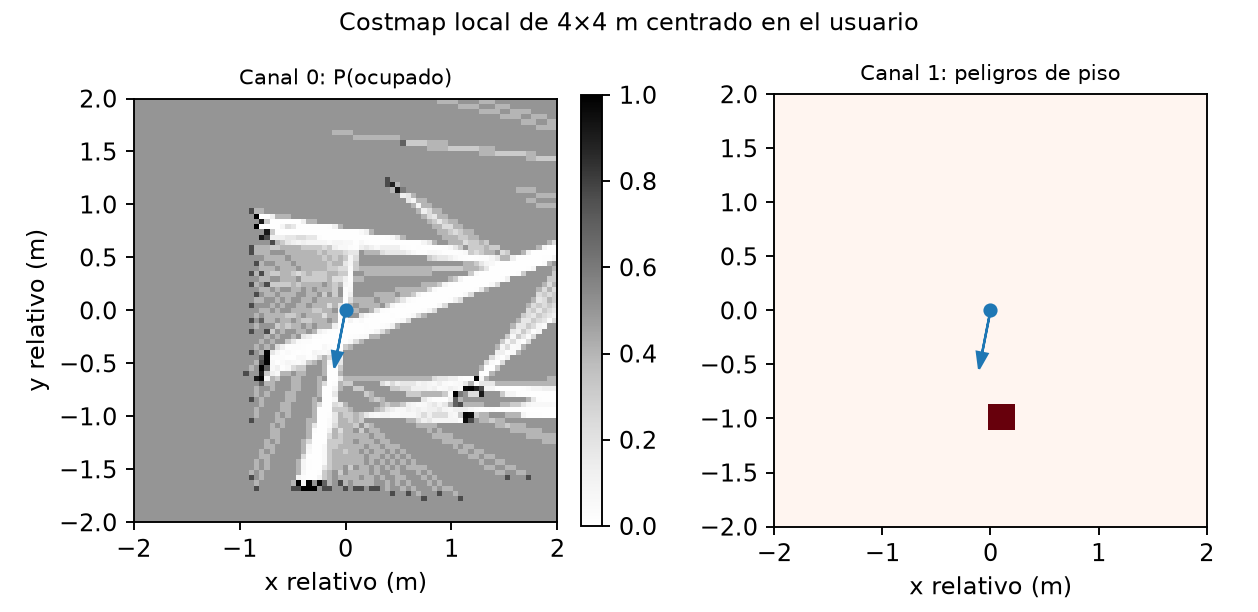
\includegraphics[width=0.85\textwidth]{Capturas_TT2/mapeo_costmap.png}
    \caption{Mapa local de $4 \times 4$~m centrado en el usuario, con la probabilidad de
    ocupación (izquierda) y los peligros de piso (derecha).}
    \label{fig:mapeo_costmap}
\end{figure}

\subsection{Del video al mapa}

Para tener mapas de muchos lugares reales sin recorrerlos todos con el prototipo se
desarrolló el script \texttt{video\_a\_mapa.py}. El script procesa videos grabados en
primera persona con el mismo flujo del sistema (visión, SLAM, Ray Casting y mapa por
bloques) y guarda el resultado. Al final genera un reporte que dice si el mapa tiene
suficiente espacio libre para usarse en el entrenamiento de la navegación y, si no,
sugiere grabar más pasadas por el mismo lugar. También trae recomendaciones de grabación,
como sostener el teléfono a la altura del pecho, caminar y girar despacio porque el giro
se estima con flujo óptico, evitar contraluces y pasar dos o más veces por cada zona
para que los \emph{landmarks} se confirmen.

\subsection{Resultados}

\textbf{Mapas con el prototipo.} \TODO{mapas construidos con el prototipo en recorridos
reales (figura y tabla con bloques, \emph{landmarks}, puertas y superficie libre), y
comparación con un plano o croquis del lugar}.

\textbf{Construcción incremental.} La Figura~\ref{fig:mapeo_evolucion} muestra cómo
evoluciona el mapa del cuarto simulado. El mapa se construye sin información previa
(RF-15); al principio solo se conocen las zonas que alcanzaron los primeros rayos y, al
terminar el recorrido, ya se distinguen el espacio libre, los obstáculos y las paredes
hacia las que el usuario caminó (RF-16). Como los dos ultrasónicos miran al frente con un
haz angosto, las paredes que solo quedan a los costados del recorrido casi no se
registran y buena parte del contorno del cuarto se queda en gris, es decir, sin conocer.

\begin{figure}[H]
    \centering
    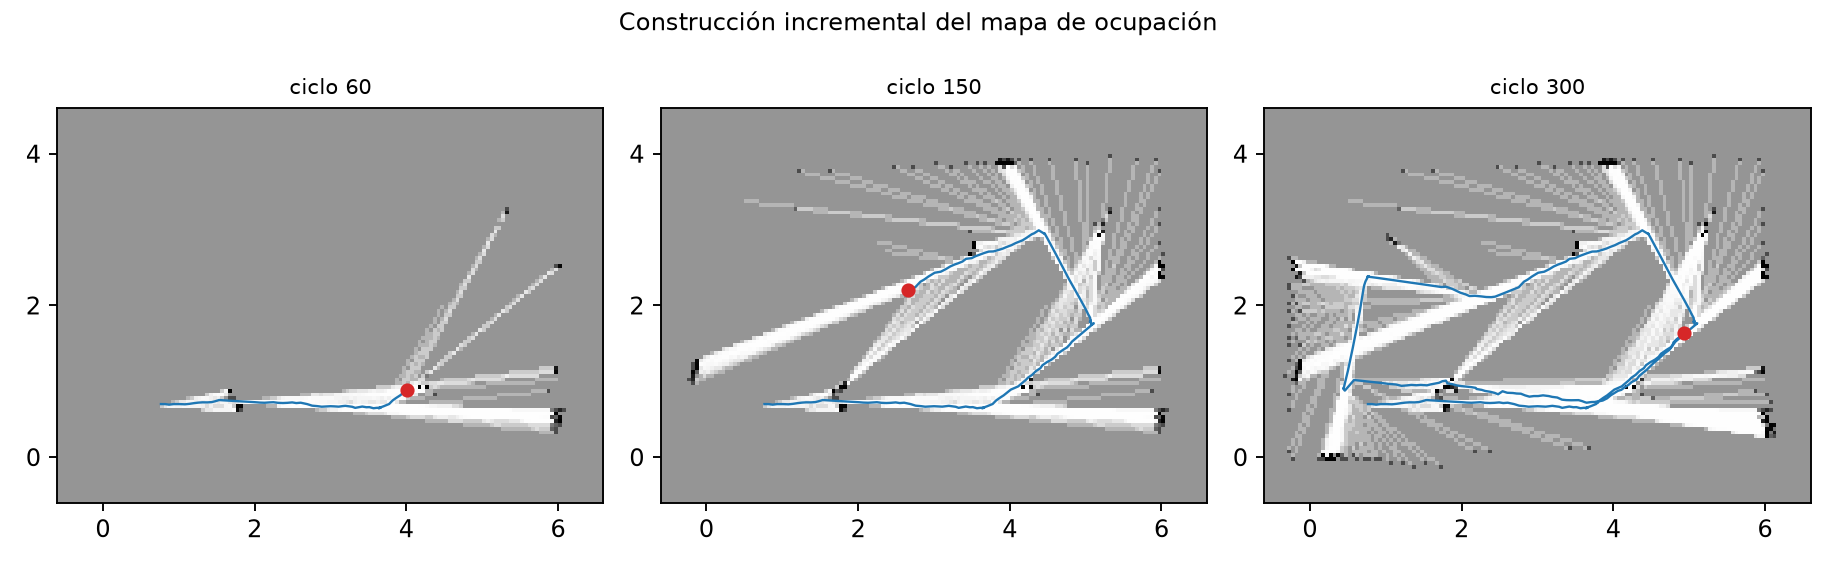
\includegraphics[width=\textwidth]{Capturas_TT2/mapeo_evolucion.png}
    \caption{Mapa de ocupación del cuarto simulado en los ciclos 60, 150 y 300. En blanco
    lo libre, en negro lo ocupado y en gris lo desconocido; la línea azul es la
    trayectoria estimada.}
    \label{fig:mapeo_evolucion}
\end{figure}

\textbf{Aporte del ultrasonido.} El banco de simulación usa el mismo montaje que el
prototipo, con dos sensores frontales paralelos separados 10~cm. Para ver qué tan buena
fue esa decisión se comparó contra otras dos disposiciones y contra el caso sin
ultrasonido (Tabla~\ref{tab:mapeo_us}). La configuración de tres sensores es la que usaba
el banco en una versión anterior, y la de sensores laterales es la que sugería la
descripción electrónica de TT1.

\begin{table}[H]
\centering
\caption{Efecto de la configuración ultrasónica (promedio de seis corridas)}
\label{tab:mapeo_us}
\renewcommand{\arraystretch}{1.2}
\begin{tabular}{|p{6.2cm}|c|c|c|}
\hline
\textbf{Configuración} & \textbf{ATE (m)} & \textbf{Precisión} &
\textbf{Exhaustividad} \\
\hline
Dos sensores frontales, como el prototipo & 0.21 & 0.60 & 0.31 \\
Tres sensores ($0^\circ$, $\pm 40^\circ$) & 0.27 & 0.48 & 0.43 \\
Dos sensores laterales ($\pm 90^\circ$) & 0.28 & 0.55 & 0.48 \\
Sin ultrasonido & 0.30 & 0.60 & 0.05 \\
\hline
\end{tabular}
\end{table}

El montaje del prototipo da la mejor localización (0.21~m) y la mejor precisión del mapa,
porque los ecos frontales coinciden con lo que ve la cámara y las paredes quedan bien
ubicadas. A cambio, registra menos superficie que las configuraciones con sensores
abiertos hacia los lados, con una exhaustividad de 0.31 contra 0.43 a 0.48. Sin
ultrasonido la exhaustividad se desploma a 0.05, porque el mapa solo registra los objetos
anclados a \emph{landmarks} y casi ninguna pared, y su precisión es alta nada más porque
marca muy pocas celdas. El resultado justifica los MB1232 sobre todo por el mapa. Abrir
un poco cada sensor hacia afuera, algo que \texttt{montaje.py} ya permite, podría
recuperar parte de la cobertura lateral, aunque se perdería el traslape central que hace
posible el cálculo estéreo del lado.

\textbf{Mapas de recorridos en video.} La Tabla~\ref{tab:mapeo_reales} resume los mapas
de los 19 videos, y las Figuras~\ref{fig:mapeo_real_pasillo} a
\ref{fig:mapeo_real_banqueta} muestran tres de ellos. Los videos no traen ultrasonido,
así que el espacio libre sale sobre todo de la huella del usuario y las celdas ocupadas
solo de los objetos anclados a \emph{landmarks}.

\begin{table}[H]
\centering
\caption{Mapas generados a partir de videos reales}
\label{tab:mapeo_reales}
\renewcommand{\arraystretch}{1.2}
\begin{tabular}{|l|c|c|c|c|c|}
\hline
\textbf{Recorrido} & \textbf{Bloques} & \textbf{Landmarks} & \textbf{Puertas} &
\textbf{Peligros} & \textbf{Libre observado (m$^2$)} \\
\hline
Calle 1 & 5 & 1 & 0 & 0 & 12.4 \\
Calle 2 & 5 & 5 & 0 & 1 & 10.6 \\
Casa & 6 & 29 & 5 & 11 & 34.5 \\
Pasillo & 9 & 25 & 13 & 1 & 45.4 \\
Plaza comercial & 13 & 26 & 6 & 4 & 38.5 \\
Oficina 1 & 8 & 23 & 11 & 1 & 19.3 \\
Oficina 2 & 4 & 12 & 9 & 0 & 20.4 \\
Video vertical & 5 & 8 & 1 & 5 & 12.7 \\
Oficina 3 & 8 & 28 & 12 & 2 & 16.9 \\
Oficina 4 & 5 & 39 & 17 & 3 & 18.3 \\
Puesto callejero & 4 & 5 & 0 & 2 & 4.2 \\
Banqueta 1 & 5 & 9 & 0 & 8 & 8.1 \\
Avenida 1 & 7 & 8 & 0 & 4 & 13.3 \\
Avenida 2 & 7 & 11 & 0 & 4 & 16.1 \\
Banqueta 2 & 8 & 16 & 0 & 13 & 37.5 \\
Esquina & 5 & 14 & 0 & 7 & 14.0 \\
Sala de maestros 1 & 4 & 4 & 2 & 0 & 1.1 \\
Sala de maestros 2 & 4 & 6 & 5 & 0 & 4.2 \\
Sala de maestros 3 & 4 & 9 & 3 & 0 & 11.5 \\
\hline
\end{tabular}
\end{table}

\begin{figure}[H]
    \centering
    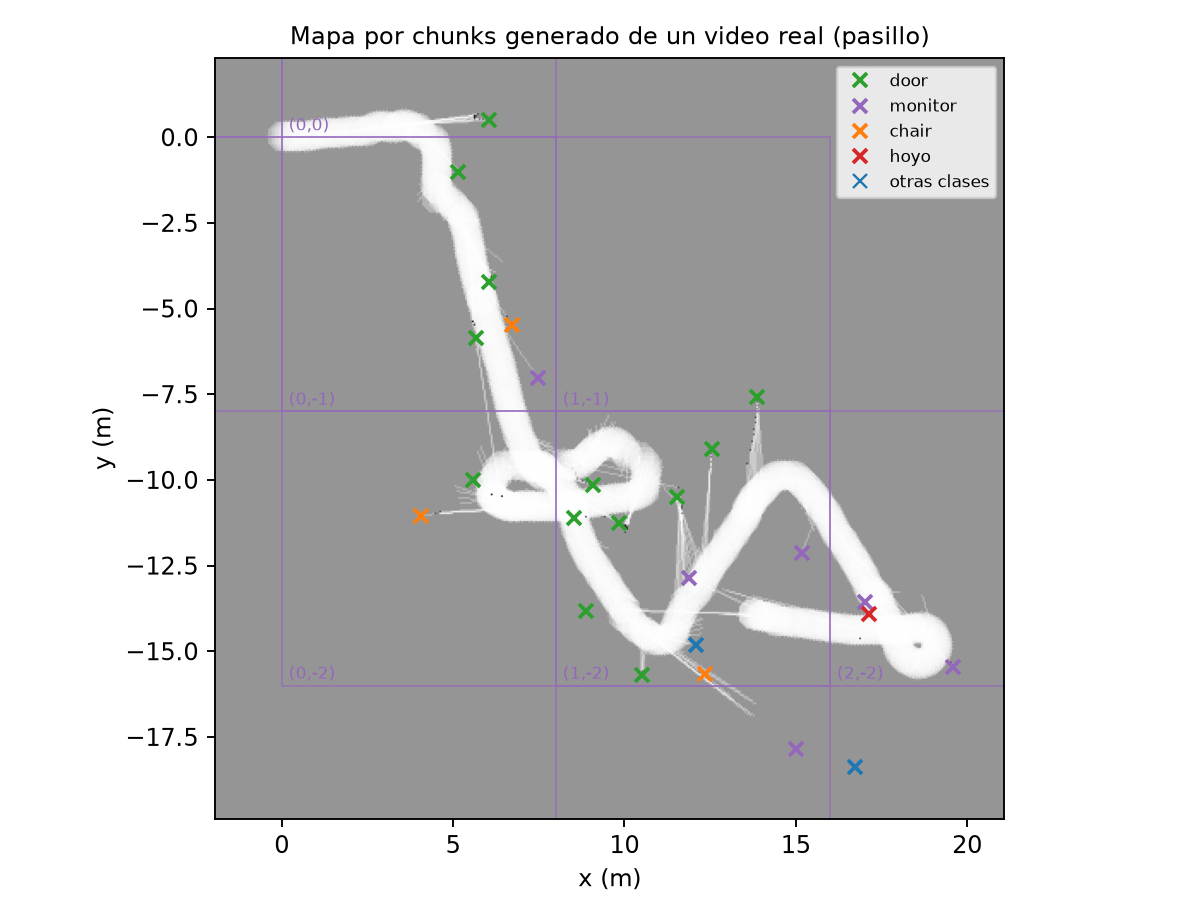
\includegraphics[width=0.8\textwidth]{Capturas_TT2/mapeo_real_pasillo.png}
    \caption{Mapa por bloques del recorrido de un pasillo. Los recuadros morados son los
    bloques de $8 \times 8$~m y las cruces, los \emph{landmarks} por clase.}
    \label{fig:mapeo_real_pasillo}
\end{figure}

\begin{figure}[H]
    \centering
    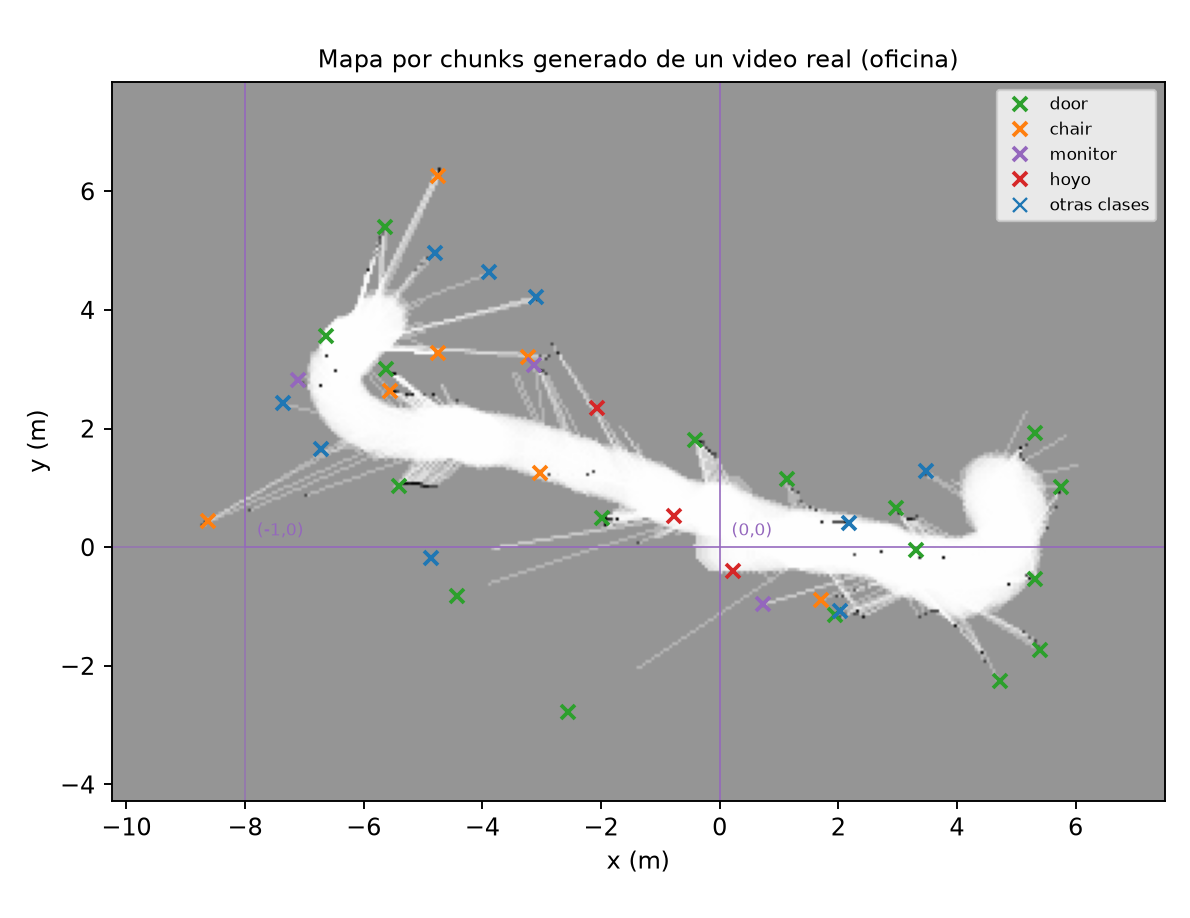
\includegraphics[width=0.8\textwidth]{Capturas_TT2/mapeo_real_oficina.png}
    \caption{Mapa por bloques del recorrido de una oficina.}
    \label{fig:mapeo_real_oficina}
\end{figure}

\begin{figure}[H]
    \centering
    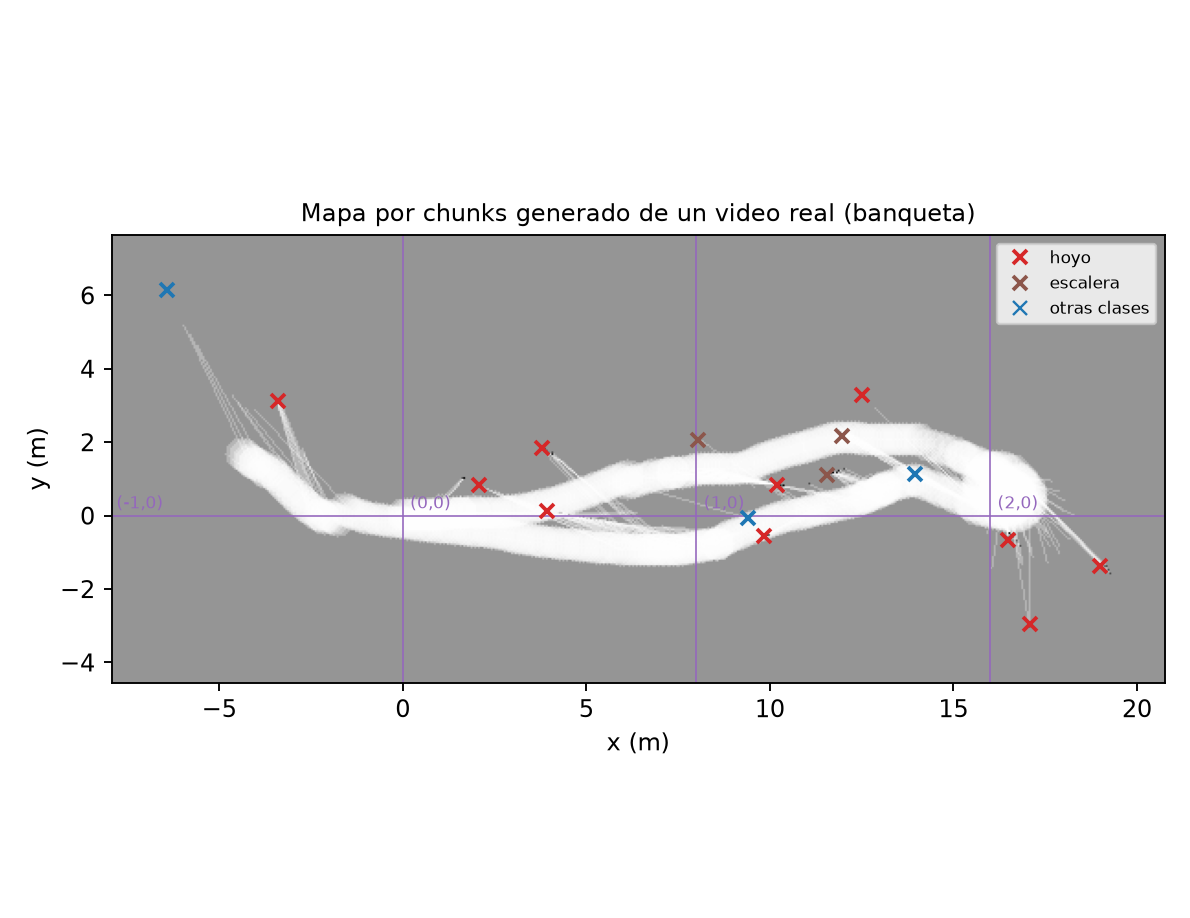
\includegraphics[width=0.8\textwidth]{Capturas_TT2/mapeo_real_banqueta.png}
    \caption{Mapa por bloques del recorrido de una banqueta, con muchos peligros de piso
    registrados.}
    \label{fig:mapeo_real_banqueta}
\end{figure}

En los recorridos de interiores las puertas son la clase más frecuente, lo cual viene
bien porque son los destinos naturales de la navegación (``llévame a la salida''). La
tabla también deja ver falsos positivos, ya que en las oficinas aparecen peligros de piso
que no son hoyos reales, probablemente porque la segmentación confunde reflejos o
cambios de textura del piso con zonas no transitables. Los mapas de calle tienen pocos
\emph{landmarks}, porque hay pocos objetos estáticos de las clases detectables, y en
cambio juntan muchos peligros de piso. En las banquetas, esos peligros pueden ser
escalones y desniveles reales que la segmentación toma por escaleras, o grietas y
manchas del pavimento; con estos datos no hay forma de separarlos.

\textbf{Persistencia.} Los 19 mapas se cargan desde disco con sus bloques,
\emph{landmarks} y valores de log-odds, y se consultan con la misma interfaz que un mapa
en memoria. Las pruebas automatizadas comprueban además que, al guardar y volver a cargar
un mapa, se conservan las celdas ocupadas, los peligros y las etiquetas de cuarto, que los
\emph{landmarks} vuelven al SLAM, que un mapa con geometría distinta se rechaza y que
descargar bloques por falta de memoria no pierde información.

\subsection{Limitaciones}

Los bloques están fijos en el mundo y no se corrigen cuando el SLAM acumula deriva, así
que un error de pose se queda ``congelado'' en el mapa. La re-localización entre
sesiones, por su parte, requiere empezar en el mismo punto y con la misma orientación
con que se creó el mapa. Los peligros de piso solo se borran cuando la cámara vuelve a
ver la zona como piso, así que un falso hoyo que quedó atrás del usuario permanece en el
mapa hasta que regrese por ahí. Los mapas de recorridos en video de la tabla anterior se
construyeron antes de agregar los rayos de piso libre, por lo que sus conteos de
peligros pueden ser algo mayores a los que daría el sistema actual.

La detección de cruce de puertas es una heurística y depende de que la puerta ya esté
confirmada como \emph{landmark}. Y cuando no hay ultrasonido, como en los mapas hechos
con video, el mapa tiene muy pocas paredes y el espacio libre se reduce a la franja por
la que caminó el usuario.


% ==============================================================================
\section{Integración de los módulos de representación}
\label{sec:dev_integracion}
% ==============================================================================

Los tres módulos anteriores trabajan en secuencia dentro del ciclo principal del
sistema. El mismo ciclo corre en el programa de la Raspberry Pi del prototipo
(\texttt{main\_pi.py}, sin interfaz gráfica), en el programa de pruebas para la
computadora portátil (\texttt{main\_lap.py}, con interfaz gráfica y entrada de cámara,
video o simulación) y en el procesamiento de videos (\texttt{video\_a\_mapa.py}). El
Algoritmo~\ref{alg:dev_representacion} resume el orden de las operaciones y sustituye
al pseudocódigo integrado de representación que se planteó en TT1
(Apéndice~\ref{apend:representa}).

\begin{center}
\captionof{algorithm}{Ciclo integrado de los módulos de representación}
\label{alg:dev_representacion}
\end{center}
\vspace{-1.8cm}
\rule{\textwidth}{0.4pt}
\vspace{-0.9cm}
\begin{algorithmic}[1]

\Statex \textbf{INICIO:}
\State mapa $\gets$ abrir\_mapa\_por\_bloques(carpeta) \Comment{crea o restaura los bloques}
\State slam $\gets$ EKF en (0, 0, 0)
\State slam.cargar\_referencias(mapa.referencias\_guardadas) \Comment{re-localización}

\Statex
\Statex \textbf{CICLO (por cada cuadro de la cámara):}
\State movimiento, cabeceo $\gets$ odometría.actualizar(cuadro) \Comment{IMU o flujo óptico}
\State detecciones $\gets$ visión.procesar(cuadro, giro = movimiento.$\Delta\theta$)
\If{toca segmentación (cada N cuadros)}
    \State peligros $\gets$ detector\_peligros.procesar(cuadro)
\EndIf
\State lecturas $\gets$ ultrasónicos.leer()
\State lecturas $\gets$ validar\_con\_ultrasonido(detecciones, lecturas, cabeceo)
\State observaciones $\gets$ fusionar(detecciones + peligros, lecturas)
\State salida $\gets$ slam.ciclo(movimiento, observaciones)
\State pose $\gets$ (salida.x, salida.y, salida.$\theta$)
\State mapa.actualizar\_con\_rayos(pose, slam.observaciones\_para\_mapa() + rayos\_sin\_eco(lecturas))
\State mapa.despejar\_huella(pose)
\State eventos $\gets$ mapa.actualizar\_posición(pose, slam.referencias)
\State cuadro\_nav $\gets$ construir\_cuadro\_navegación(slam, mapa, detecciones, lecturas)
\State entregar cuadro\_nav y eventos a navegación, alertas e interacción

\Statex
\Statex \textbf{AL TERMINAR:}
\State mapa.guardar\_todo();\; mapa.guardar\_referencias(slam.exportar\_referencias())

\end{algorithmic}
\vspace{-0.9cm}
\rule{\textwidth}{0.4pt}

\subsection{Funcionamiento con video}

Las Figuras~\ref{fig:cap_oficina_1} a \ref{fig:cap_oficina_3} son capturas de la
interfaz de \texttt{main\_lap.py} mientras procesa el recorrido de una oficina grabado
con un teléfono. A la izquierda de cada captura está la imagen de la cámara con las
detecciones; en verde los objetos estáticos y en rojo los marcados como móviles, junto
con su clase, el estado de las puertas y la distancia estimada. A la derecha está el
mapa global por bloques, con los \emph{landmarks} etiquetados, la pose del usuario
(punto rojo con su orientación) y su elipse de incertidumbre. Abajo aparece la barra
de navegación con la distancia libre y el riesgo de cada sector, y la alerta del
momento.

\begin{figure}[H]
    \centering
    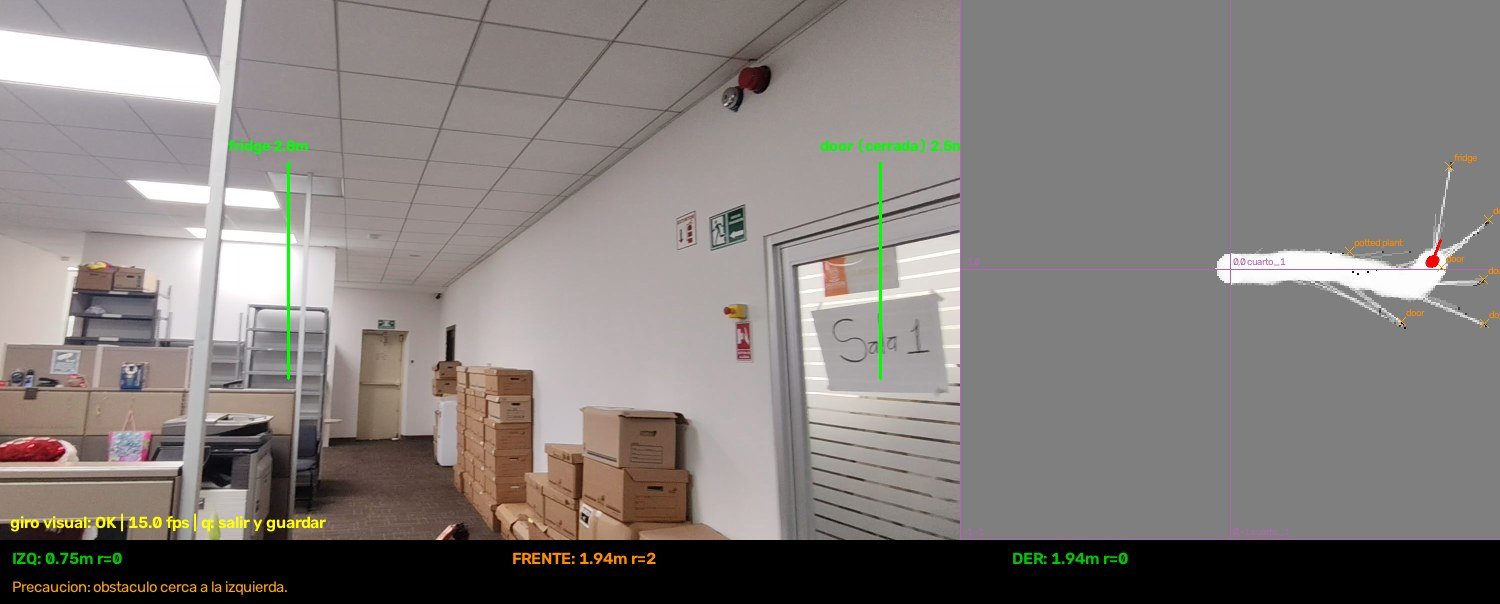
\includegraphics[width=\textwidth]{Capturas_TT2/cap_oficina_f241.jpg}
    \caption{Inicio del recorrido. Se detectan una puerta cerrada a 2.5~m y un
    refrigerador, el mapa empieza a registrar la franja recorrida y la barra avisa de un
    obstáculo a 0.75~m a la izquierda.}
    \label{fig:cap_oficina_1}
\end{figure}

\begin{figure}[H]
    \centering
    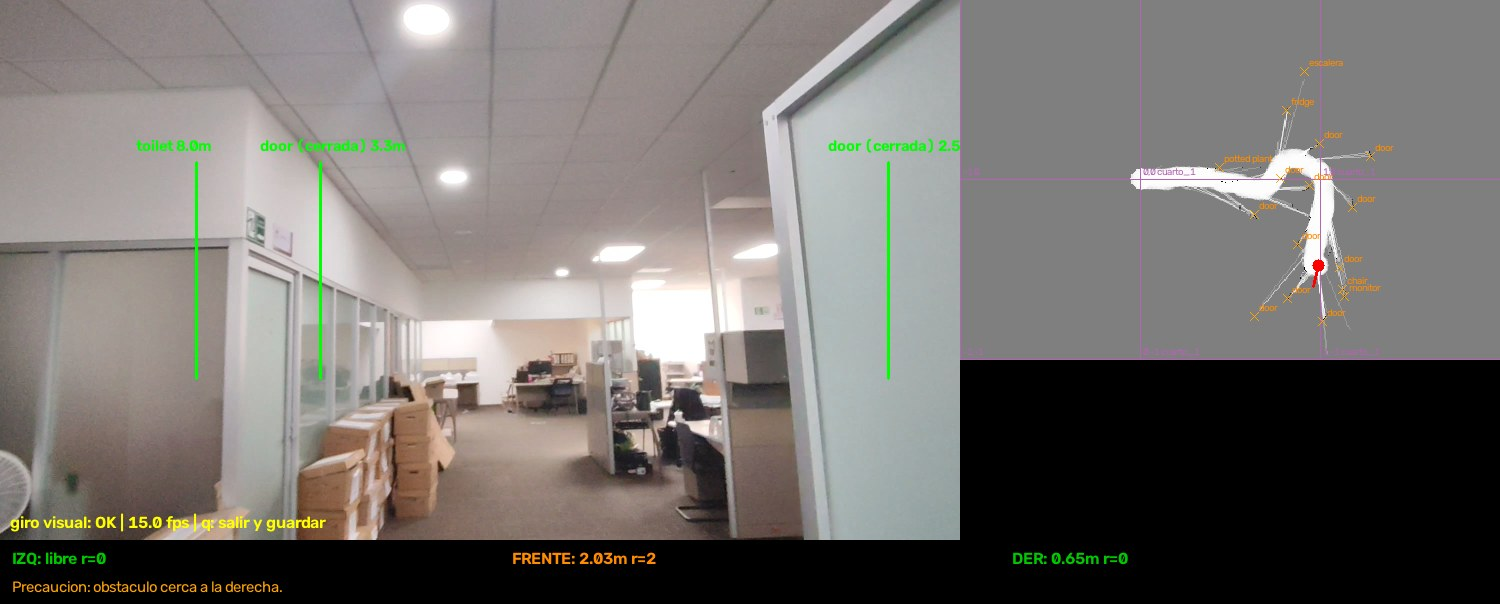
\includegraphics[width=\textwidth]{Capturas_TT2/cap_oficina_f481.jpg}
    \caption{Al girar hacia el pasillo, el SLAM ya mantiene varias puertas como
    \emph{landmarks} y el mapa muestra el cambio de dirección.}
    \label{fig:cap_oficina_2}
\end{figure}

\begin{figure}[H]
    \centering
    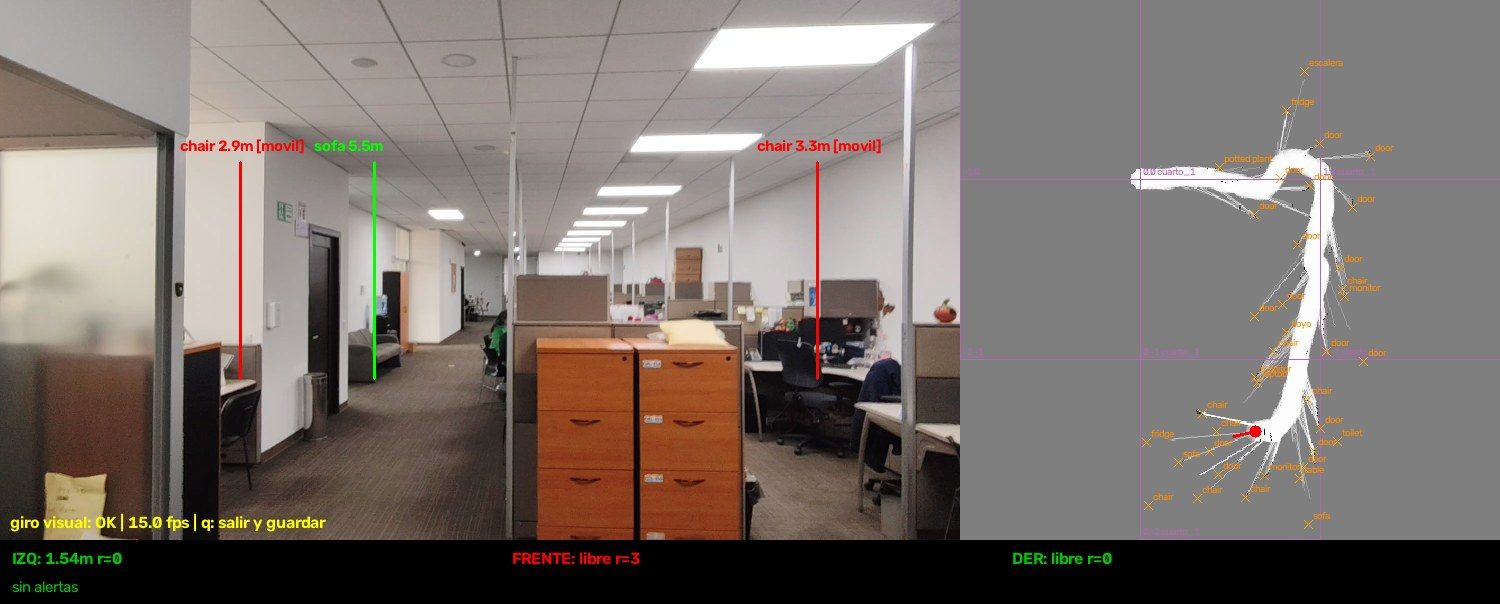
\includegraphics[width=\textwidth]{Capturas_TT2/cap_oficina_f901.jpg}
    \caption{Final del recorrido, con siete bloques y 39 \emph{landmarks} confirmados.
    Dos sillas aparecen como móviles por un error del rastreador al avanzar el
    usuario.}
    \label{fig:cap_oficina_3}
\end{figure}

En las capturas se ven también errores de la percepción que llegan a la
representación. En la Figura~\ref{fig:cap_oficina_2} aparece un inodoro a 8~m que no
existe, y en la Figura~\ref{fig:cap_oficina_3} dos sillas que no se mueven se marcan como
móviles, porque el rastreador compensa el giro del usuario pero no su avance. Las reglas
del SLAM contienen el daño, ya que los objetos móviles no se usan como \emph{landmarks}
y los falsos positivos aislados no llegan a los avistamientos necesarios para
confirmarse.

\subsection{Funcionamiento en el prototipo}

\TODO{capturas o registros de \texttt{main\_pi.py} durante un recorrido con el
prototipo: mapa resultante, \emph{landmarks}, alertas emitidas y comentarios del
recorrido}.

\subsection{Tiempos de procesamiento}

La Tabla~\ref{tab:tiempos_ciclo} desglosa el tiempo promedio por ciclo. La columna de
la computadora portátil se midió al procesar el video de la oficina (456 cuadros, uno de
cada dos del video original) con todos los modelos en CPU; la de la Raspberry Pi
corresponde al prototipo en operación.

\begin{table}[H]
\centering
\caption{Tiempo promedio por ciclo}
\label{tab:tiempos_ciclo}
\renewcommand{\arraystretch}{1.2}
\begin{tabular}{|p{7.4cm}|c|c|}
\hline
\textbf{Etapa} & \textbf{Apple M4 (ms)} & \textbf{Raspberry Pi (ms)} \\
\hline
Estimación de giro y caminata por flujo óptico & 5.4 & \TODO{} \\
Detección de objetos (YOLOv8s-seg) & 92.4 & \TODO{} \\
Segmentación de peligros y puertas (SegFormer, amortizado) & 77.5 & \TODO{} \\
\hline
SLAM (EKF, asociación y gestión de \emph{landmarks}) & 0.27 & \TODO{} \\
Ray Casting y actualización del mapa por bloques & 0.23 & \TODO{} \\
Construcción del cuadro de navegación & 0.51 & \TODO{} \\
\hline
\textbf{Subtotal de los módulos de representación} & \textbf{1.01} & \TODO{} \\
\hline
\end{tabular}
\end{table}

Los módulos de representación se llevan alrededor de un milisegundo por ciclo en la
computadora portátil, menos del 1\,\% del tiempo total. Por sí solos podrían correr a
cientos de hertz, muy por encima de los 10~Hz que pide RNF-03; el cuello de botella es la
percepción visual. Por eso el SLAM y el mapa siguen actualizándose con la odometría en
los ciclos en que la visión no entrega resultados, y la segmentación solo se ejecuta cada
cierto número de cuadros. En la Raspberry Pi el ciclo completo corre a \TODO{frecuencia
del ciclo completo en la Raspberry Pi}.

\subsection{Cumplimiento de requerimientos}

La Tabla~\ref{tab:req_representacion} relaciona los requerimientos de los módulos de
representación con su estado.

\begin{longtable}{|p{1.6cm}|p{4.2cm}|p{2.4cm}|p{6.2cm}|}
\caption{Estado de los requerimientos de los módulos de representación}
\label{tab:req_representacion} \\
\hline
\textbf{Req.} & \textbf{Descripción breve} & \textbf{Estado} & \textbf{Evidencia} \\
\hline
\endfirsthead
\hline
\textbf{Req.} & \textbf{Descripción breve} & \textbf{Estado} & \textbf{Evidencia} \\
\hline
\endhead
RF-14 & Estimación continua de la pose & Cumplido & EKF con ATE de 0.21~m en
simulación y error acotado con odometría sesgada (Tabla~\ref{tab:slam_deriva}). \\
\hline
RF-15 & Mapa incremental sin mapa previo & Cumplido &
Figura~\ref{fig:mapeo_evolucion} y mapas de 19 videos reales. \\
\hline
RF-16 & Zonas libres y ocupadas & Cumplido & Mapa log-odds con tres estados, capa de
peligros y mapa local de dos canales. \\
\hline
RF-17 & Actualización dinámica & Cumplido & Los obstáculos nuevos aparecen en el mapa;
los que desaparecen se liberan con ecos precisos y los falsos peligros de piso, con los
rayos de piso libre (Secciones~\ref{sec:dev_ray} y \ref{sec:dev_mapeo}). \\
\hline
RNF-03 & Mapa a 10~Hz o más & \TODO{} & 1~ms por ciclo en la computadora portátil
(Tabla~\ref{tab:tiempos_ciclo}); \TODO{frecuencia en la Raspberry Pi}. \\
\hline
RNF-05 & Hardware limitado & \TODO{} & Estado de pose de tamaño fijo y memoria acotada a
25 bloques (unos 3~MB); \TODO{uso de memoria y CPU en la Raspberry Pi}. \\
\hline
RNF-09 & Comportamiento conservador & Cumplido & Confianza que baja sin correcciones
(Figura~\ref{fig:slam_incertidumbre}) y distancia mínima por sector. \\
\hline
RNF-13 & Operación sin internet & Cumplido & Ningún módulo de representación necesita
conexión y los mapas se guardan localmente. \\
\hline
RNF-14 & Modularidad & Cumplido & Comunicación solo por las estructuras de
\texttt{interfaces.py}; el mismo código trabaja con cámara, video y simulación. \\
\hline
\end{longtable}


% ==============================================================================
\section{Módulo de navegación}
\label{sec:dev_nav}
% ==============================================================================

\subsection{Descripción}

El módulo de navegación decide, paso a paso, qué debe hacer el usuario para llegar a
su destino: avanzar, girar a la izquierda, girar a la derecha o detenerse. La decisión
la toma un agente de aprendizaje por refuerzo profundo entrenado en simulación con el
algoritmo PPO, tal como se planteó en TT1. Alrededor del agente se construyeron tres
piezas que no estaban en el diseño original: un ejecutor que administra la sesión y
traduce las acciones en frases, una capa de seguridad determinística que puede
anular al agente y un planificador que anticipa la ruta completa para mostrarla en la
interfaz. El módulo cubre los requerimientos RF-18 a RF-21 y RF-23.

Los destinos ya no provienen de un servicio de cartografía. Cuando el usuario pide
``llévame a la salida'', el ejecutor busca entre los \emph{landmarks} del SLAM el más
cercano con la etiqueta correspondiente (puerta, en este caso) y lo toma como meta.
También se acepta un punto explícito del mapa, lo cual se usa durante las pruebas.

\subsection{Entorno de entrenamiento}

El agente se entrena en un entorno propio construido con Gymnasium
(\texttt{navigation/nav\_env.py}). Cada episodio genera un mundo nuevo de uno de tres
tipos:

\begin{itemize}
    \item \textbf{Cuarto} (40\,\% de los episodios): un rectángulo de 4 a 9~m por 3.5 a
    7~m con entre dos y cinco muebles, hasta un peligro de piso y hasta una persona en
    movimiento.
    \item \textbf{Dos cuartos con puerta} (35\,\%): dos cuartos separados por una pared
    con un vano de 0.9 a 1.3~m. El inicio está en un cuarto y la meta en el otro, de
    modo que el agente debe encontrar la puerta.
    \item \textbf{Exterior} (25\,\%): un área abierta de 10 a 18~m por 8 a 14~m con
    postes dispersos, de una a tres coladeras y hasta dos personas.
\end{itemize}

Las personas se desplazan entre 5 y 12~cm por paso, rebotan en los límites y de vez
en cuando cambian de dirección. Los peligros de piso no bloquean los rayos, igual que
en el sistema real, donde un hoyo no produce eco ni detiene la vista: el agente solo
los conoce por la distancia por sector que le llega en la observación. Además de los
mundos generados, en aproximadamente la mitad de los episodios se usa uno de los 19
mapas reales obtenidos de video (Sección~\ref{sec:dev_mapeo}). Para ello, las celdas
ocupadas se convierten en obstáculos circulares, la capa de peligros en coladeras, y
el inicio y la meta se eligen dentro de la misma zona libre conexa, con al menos
30~cm de holgura respecto a cualquier obstáculo.

\subsection{Acciones, observación y recompensa}

Las acciones son las cuatro definidas en TT1: avanzar 0.30~m, girar $20^\circ$ a la
izquierda, girar $20^\circ$ a la derecha y detenerse.

La observación es donde más se apartó la implementación del diseño original. El
vector de ocho valores planteado en TT1 ($d_{\text{front}}$, $d_{\text{left}}$,
$d_{\text{right}}$, $\phi_{\text{goal}}$, $d_{\text{goal}}$ y los tres riesgos) se
implementó y se comparó contra una observación extendida de 24 valores, descrita en la
Tabla~\ref{tab:nav_obs}. Con el mismo presupuesto de entrenamiento, la observación
extendida obtuvo 85.8\,\% de episodios exitosos contra 44.2\,\% de la original
(Figura~\ref{fig:nav_comparacion}). La diferencia se concentra en los mundos con
puerta: con solo tres distancias por sector, el agente no ``ve'' el hueco de la puerta
y fracasa en nueve de cada diez intentos.

\begin{table}[H]
\centering
\caption{Componentes de la observación extendida (24 valores normalizados)}
\label{tab:nav_obs}
\renewcommand{\arraystretch}{1.25}
\begin{tabular}{|c|p{11.8cm}|}
\hline
\textbf{Valores} & \textbf{Contenido} \\
\hline
11 & Distancia libre en 11 direcciones entre $-100^\circ$ y $+100^\circ$, divididas
entre el alcance máximo de 4~m. \\
\hline
3 & Distancia al peligro de piso más cercano en cada sector (frente, izquierda,
derecha), divididas entre 3~m. \\
\hline
3 & Nivel de riesgo por sector, dividido entre 3. \\
\hline
3 & Dirección a la meta como $\sin\phi_{\text{goal}}$ y $\cos\phi_{\text{goal}}$, y
distancia a la meta acotada a 10~m. \\
\hline
4 & Acción anterior en codificación \emph{one-hot}. \\
\hline
\end{tabular}
\end{table}

\begin{figure}[H]
    \centering
    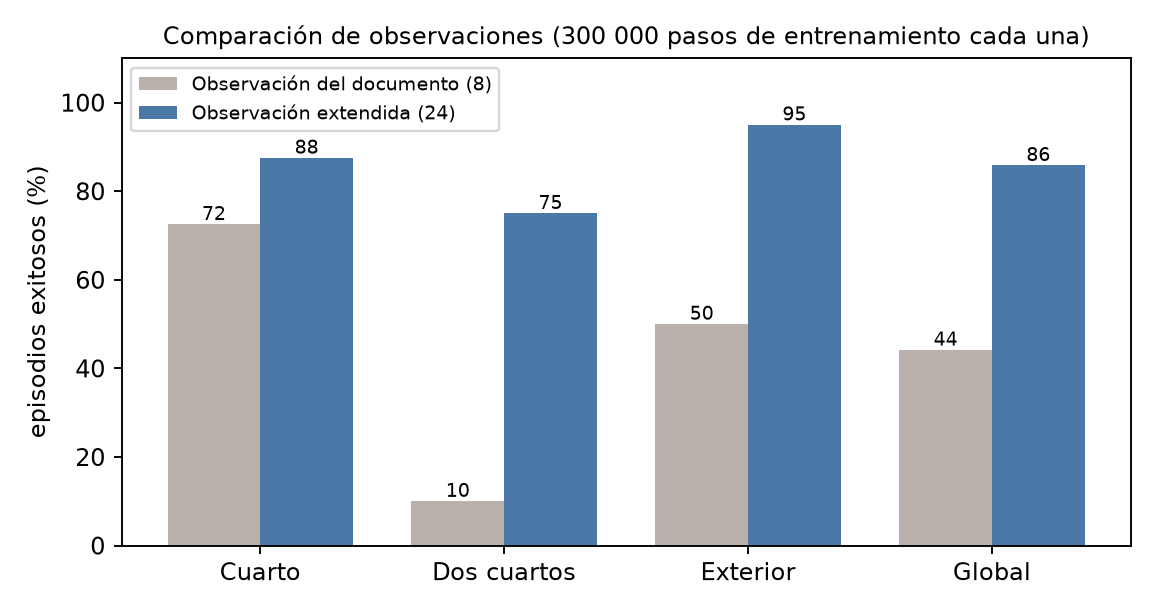
\includegraphics[width=0.78\textwidth]{Capturas_TT2/nav/nav_comparacion_obs.png}
    \caption{Porcentaje de episodios exitosos con la observación del documento y con la
    observación extendida, tras 300\,000 pasos de entrenamiento cada una.}
    \label{fig:nav_comparacion}
\end{figure}

La recompensa sigue la estructura de TT1, pero con escalas ajustadas. Con los
coeficientes originales, la penalización por riesgo pesaba tanto que el agente
aprendía a quedarse quieto. La versión final es:

\[
r_t = -0.1 + 4\,(d_{t-1} - d_t) - 0.15\, r_{\text{front}}
      + \begin{cases}
      +100 & \text{si llega a menos de 0.45~m de la meta} \\
      -100 & \text{si choca o cae en un peligro de piso} \\
      +0.5 & \text{si se detiene con una persona a menos de 1.2~m enfrente} \\
      -0.3 & \text{si se detiene sin motivo}
      \end{cases}
\]

donde $d_t$ es la distancia a la meta. El término de detenerse se agregó para que la
acción tuviera una función clara: esperar a que una persona termine de cruzar.

Para reducir la diferencia entre la simulación y el sistema real se añadió ruido de
5\,\% a las distancias, de $2^\circ$ al ángulo de la meta y, en el 8\,\% de los rayos
bloqueados, se reporta el alcance máximo como si estuvieran libres. Esta última
perturbación imita lo que ocurre en el mapa real, donde un rayo delgado puede colarse
entre dos celdas de eco separadas (Sección~\ref{sec:dev_ray}) y reportar libre un
frente bloqueado.

\subsection{Entrenamiento}

El agente se entrena con la implementación de PPO de Stable-Baselines3 sobre
PyTorch, con ocho entornos en paralelo. La Tabla~\ref{tab:nav_ppo} resume los
hiperparámetros. El modelo final se entrenó durante 8 millones de pasos. Se exporta en
dos formatos: el archivo completo de Stable-Baselines3, que se usa en la computadora
portátil, y un archivo con solo los pesos de la red del actor, con el que la
Raspberry Pi ejecuta la inferencia en NumPy sin instalar PyTorch. Se verificó que
ambos formatos eligen la misma acción en 500 observaciones aleatorias.

\begin{table}[H]
\centering
\caption{Hiperparámetros de PPO}
\label{tab:nav_ppo}
\renewcommand{\arraystretch}{1.2}
\begin{tabular}{|l|c|}
\hline
\textbf{Parámetro} & \textbf{Valor} \\
\hline
Red del actor y del crítico & dos capas ocultas de 128 neuronas, \emph{tanh} \\
Pasos por actualización (por entorno) & 2048 \\
Tamaño de lote & 512 \\
Factor de descuento $\gamma$ & 0.995 \\
$\lambda$ de GAE & 0.95 \\
Coeficiente de entropía & 0.01 \\
Tasa de aprendizaje & $3 \times 10^{-4}$ \\
Recorte de PPO & 0.2 \\
\hline
\end{tabular}
\end{table}

El modelo pasó por varias iteraciones, evaluadas siempre con el mismo protocolo. Un
primer modelo entrenado solo en mundos generados alcanzó 99.2\,\% de éxito en ellos.
Al incorporar los mapas de video, el peor caso fue un pasillo de oficina muy angosto y
lleno de muebles (v09), donde varios reentrenamientos con más pasos o con otra mezcla
de mapas no lograron superar al modelo vigente. Al revisar ese caso se encontró un
error en el entrenador: en mapas densos el inicio o la meta podían quedar encima de un
obstáculo, lo que producía choques imposibles de evitar. Con el muestreo corregido, el
modelo vigente subió de 82.5 a 85\,\% en ese mapa, y se comprobó que retirar v09 del
entrenamiento empeora el desempeño en pasillos densos, por lo que se conservó en la
mezcla.

\subsection{Ejecución en el dispositivo}

El ejecutor (\texttt{navigation/navigator.py}) es la parte del módulo que corre en el
dispositivo. Mantiene el estado de la sesión (en espera, activa o pausada) con los
mensajes literales del Algoritmo 11 de TT1, recibe los comandos ya interpretados por
el PLN y, en cada ciclo, construye la observación a partir del cuadro de navegación y
del mapa. Para que esa observación se parezca a la del entrenamiento, cada uno de los
11 rayos es el mínimo de un abanico de tres sub-rayos separados $6^\circ$, y las
distancias a los peligros se leen del segundo canal del mapa local.

Sobre la decisión del agente actúan varias reglas fijas:

\begin{itemize}
    \item \textbf{Capa de seguridad.} Si el agente indica avanzar y la distancia libre
    al frente es menor que 0.80~m, ya sea según el mapa o según la visión, la orden se
    reemplaza por un giro. El umbral es el mismo de la alerta crítica, de modo que el
    usuario nunca escucha ``Deténgase'' y ``Avance'' en el mismo instante. El sentido
    del giro se mantiene durante un máximo de ocho giros seguidos (unos $160^\circ$),
    para no alternar izquierda y derecha en una esquina.
    \item \textbf{Ritmo de decisión.} El agente decide una vez por segundo, salvo que
    haya una alerta crítica, en cuyo caso decide de inmediato.
    \item \textbf{Frases.} Cada acción se traduce con las frases exactas de TT1:
    ``Avance N metros'', ``Gire ligeramente a la izquierda'' (giros de hasta
    $45^\circ$), ``Gire a la izquierda N grados'' o ``Deténgase''. La distancia de
    avance se limita a lo que el mapa ve libre y, si la confianza del SLAM baja de
    0.35, a un metro. El aviso ``Está cerca de su destino'' se dice una sola vez por
    destino.
    \item \textbf{Llegada.} La sesión termina cuando la pose queda a menos de 0.6~m de
    la meta o cuando la cámara ve el objeto buscado a menos de 1~m enfrente. La
    segunda condición se agregó porque, sin odometría, la pose deriva y el usuario
    podía quedarse dando vueltas junto al objeto.
    \item \textbf{Bloqueo.} Si en 20~s la distancia a la meta no disminuye al menos
    30~cm, el sistema avisa que no encuentra un paso libre y sugiere pedir otra ruta.
\end{itemize}

El Algoritmo~\ref{alg:dev_nav} resume un ciclo del ejecutor.

\begin{center}
\captionof{algorithm}{Ciclo del ejecutor de navegación}
\label{alg:dev_nav}
\end{center}
\vspace{-1.8cm}
\rule{\textwidth}{0.4pt}
\vspace{-0.9cm}
\begin{algorithmic}[1]

\Statex \textbf{ENTRADA:} cuadro\_nav, mapa, alertas
\Statex \textbf{SALIDA:} lista de mensajes para la salida de voz

\Statex
\If{sesión no está activa}
    \State \Return []
\EndIf
\State d $\gets$ distancia(pose, meta)
\If{d $< 0.6$ m O la cámara ve el objeto meta a menos de 1 m}
    \State sesión $\gets$ ``en\_espera''
    \State \Return [``Ha llegado a su destino.'']
\EndIf
\If{no hay alerta crítica Y pasó menos de 1 s desde la última decisión}
    \State \Return []
\EndIf
\State obs $\gets$ construir\_observación(cuadro\_nav, mapa, meta, acción\_previa)
\State acción $\gets$ política(obs)
\If{acción = avanzar Y distancia\_libre\_al\_frente $< 0.80$ m}
    \State acción $\gets$ giro\_forzado() \Comment{con histéresis de sentido}
\EndIf
\State texto $\gets$ frase(acción, d, $\phi_{\text{goal}}$, distancia\_libre, confianza)
\If{texto es nuevo O pasaron más de 3.5 s desde la última indicación}
    \State agregar texto a mensajes
\EndIf
\If{la distancia a la meta no bajó 0.3 m en 20 s}
    \State agregar aviso de bloqueo a mensajes
\EndIf
\State \Return mensajes

\end{algorithmic}
\vspace{-0.9cm}
\rule{\textwidth}{0.4pt}

\subsection{Planificador de ruta}

El agente decide solo el siguiente paso, lo cual dificulta saber hacia dónde va.
Para visualizarlo, el planificador (\texttt{navigation/route\_planner.py}) simula al
agente sobre el mapa actual desde la pose del usuario, sin moverlo, y registra los
puntos por los que pasaría hasta llegar, quedar atascado o agotar 240 pasos. La ruta
resultante se clasifica como ``llega'', ``bloqueada'' o ``larga'' y se dibuja en la
interfaz. Un plan tarda unos 7~ms; se recalcula cada dos segundos en un hilo aparte, o
de inmediato si llega una alerta crítica. Como las puertas se registran sobre la
pared, cuando la meta cae en una celda ocupada el planificador la traslada a la celda
libre más cercana. La ruta es informativa: la decisión que se le comunica al usuario
sigue siendo la del ejecutor.

\subsection{Resultados}

\textbf{Evaluación del modelo.} El modelo final se evaluó en 880 episodios: 40 en
cada tipo de mundo generado y 40 en cada uno de los 19 mapas reales, con semillas
distintas a las del entrenamiento. Llegó a la meta en el 97.8\,\% de los episodios,
chocó en el 2.0\,\%, nunca cayó en un peligro de piso y solo un episodio agotó el
límite de pasos. Los episodios exitosos tomaron en promedio 27 pasos. La
Figura~\ref{fig:nav_eval} muestra el desglose por mundo; el único mapa por debajo del
90\,\% es el pasillo denso v09 (85\,\%).

\begin{figure}[H]
    \centering
    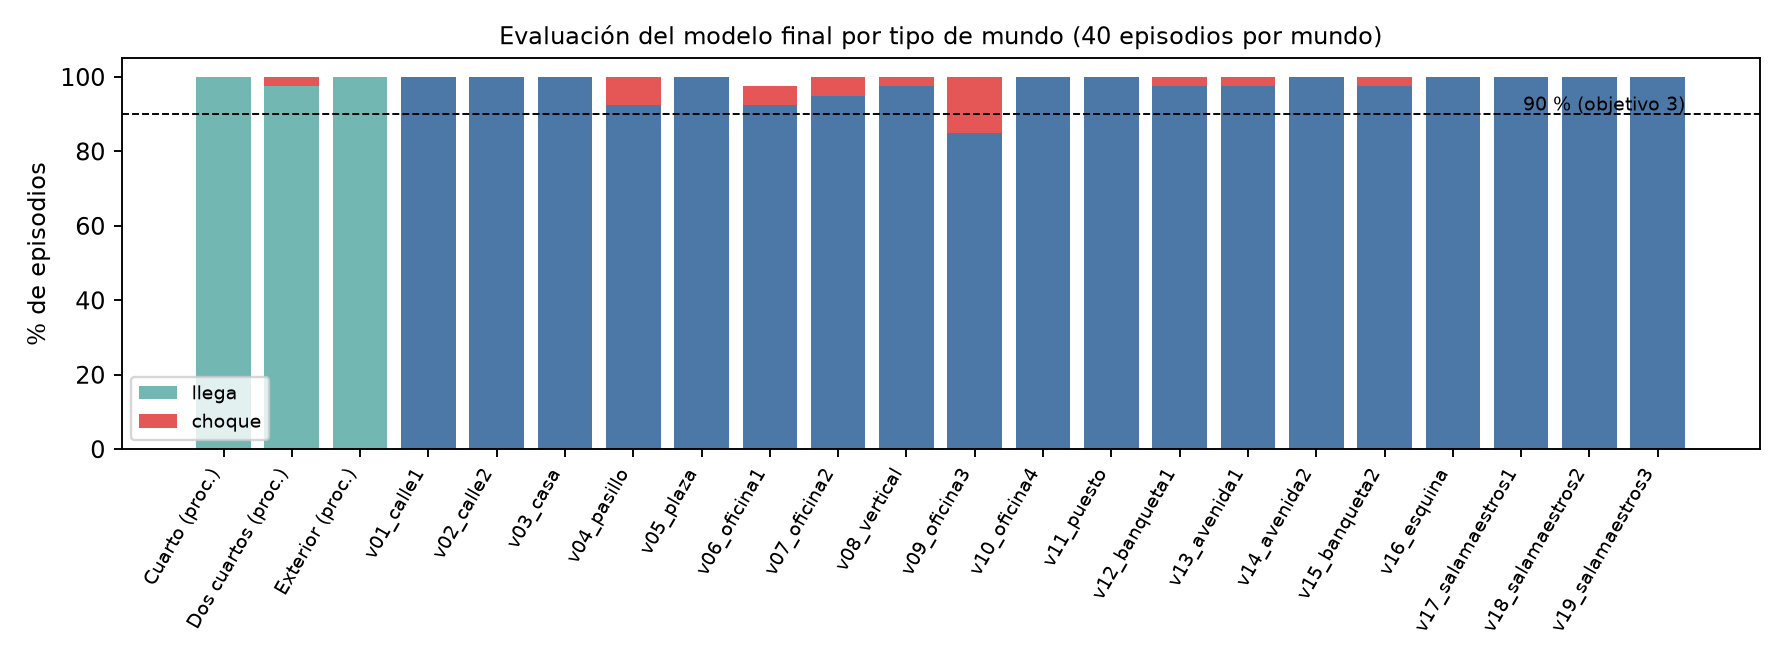
\includegraphics[width=\textwidth]{Capturas_TT2/nav/nav_eval_mundos.png}
    \caption{Porcentaje de episodios exitosos y con choque por mundo. En verde claro,
    mundos generados; en azul, mapas obtenidos de videos reales.}
    \label{fig:nav_eval}
\end{figure}

La Figura~\ref{fig:nav_episodios} muestra un episodio de cada tipo de mundo generado.
En el de dos cuartos, el agente se dirige primero hacia la puerta y cruza el vano; en
el exterior se aleja de las coladeras, aunque estas no aparecen en sus rayos.

\begin{figure}[H]
    \centering
    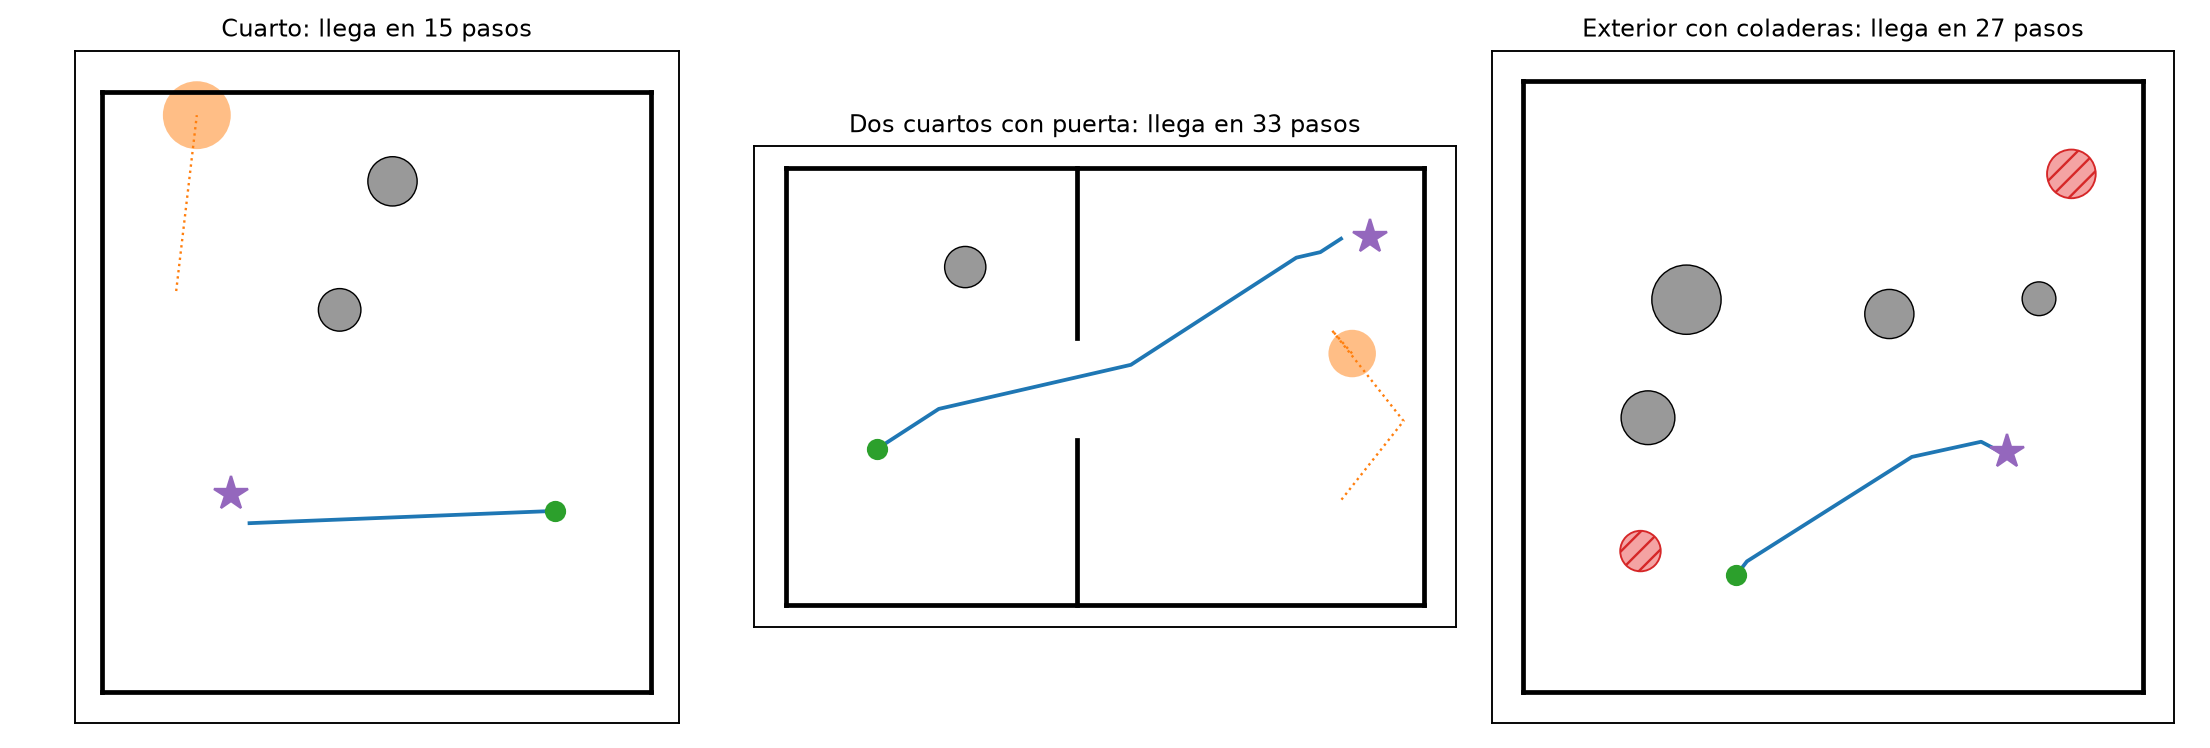
\includegraphics[width=\textwidth]{Capturas_TT2/nav/nav_episodios.png}
    \caption{Episodios del modelo final. Punto verde: inicio; estrella: meta; gris:
    obstáculos; rojo rayado: peligros de piso; naranja: persona en movimiento y su
    recorrido.}
    \label{fig:nav_episodios}
\end{figure}

\textbf{Sesiones completas en lazo cerrado.} La evaluación anterior mide al agente
dentro de su propio simulador. Para probar la cadena completa se ejecutaron sesiones
en el cuarto simulado con todos los módulos reales: sensores simulados, SLAM, mapa,
PLN, ejecutor y salida amigable. Un usuario virtual primero recorre el cuarto para
construir el mapa, después pide un destino por texto y a partir de ahí hace
exactamente lo que le indica el sistema. Se realizaron 20 sesiones (cinco semillas por
cuatro destinos) y en cada una se midió la distancia real entre el usuario y la
superficie del objeto en el momento en que el sistema anunció la llegada.

El sistema anunció la llegada en las 20 sesiones y el usuario nunca chocó, pero solo
en 7 quedó a menos de 1~m del objeto y en 12 a menos de 1.5~m. Al registrar qué
condición disparó cada llegada se encontró la causa (Tabla~\ref{tab:nav_lazo}): en 17
sesiones la llegada la decidió la regla de percepción, porque en un solo cuadro la
estimación monocular ubicó al objeto a menos de 1~m cuando en realidad estaba hasta a
2.5~m. Las tres llegadas decididas por la distancia en el mapa terminaron a menos de
0.8~m del objeto.

También se revisó si la validación con los ultrasónicos intervino en esas llegadas.
En 16 de las 17 el objeto quedaba fuera del cono angosto de los sensores (unos
$\pm 20^\circ$, mientras que la regla acepta objetos hasta $\pm 60^\circ$) o por
debajo del haz, así que el ultrasonido no pudo confirmar ni contradecir la distancia.
La única llegada con el objeto confirmado por ambos sensores terminó a 0.99~m, que es
una llegada correcta.

\begin{table}[H]
\centering
\caption{Sesiones en lazo cerrado según la condición que disparó la llegada}
\label{tab:nav_lazo}
\renewcommand{\arraystretch}{1.2}
\begin{tabular}{|p{5.2cm}|c|c|c|}
\hline
\textbf{Condición de llegada} & \textbf{Sesiones} & \textbf{Distancia real promedio}
& \textbf{A menos de 1~m} \\
\hline
Pose a menos de 0.6~m de la meta & 3 & 0.55~m & 3 \\
Objeto visto a menos de 1~m & 17 & 1.56~m & 4 \\
\hline
\textbf{Total} & \textbf{20} & & \textbf{7} \\
\hline
\end{tabular}
\end{table}

La regla de percepción resolvió un problema real, pero tal como está implementada es
demasiado sensible: basta un cuadro con un error monocular de 25 a 50\,\% para terminar
la sesión antes de tiempo. Exigir la condición durante varios cuadros seguidos, pedir
que el ultrasonido la confirme cuando el objeto está dentro de su cono, o combinarla
con la distancia en el mapa debería corregirlo.

La Figura~\ref{fig:nav_sesion} muestra una de estas sesiones. El usuario pidió
``llévame al sillón'' y en el paso 45 apareció una caja a 1.2~m delante de él. El
planificador cambió la ruta para pasar por debajo de la caja y el usuario siguió las
indicaciones hasta quedar a 0.75~m del sillón, donde la regla de percepción dio por
terminada la sesión. En corridas anteriores de la misma prueba se observó que el
primer plan después de la caja a veces todavía la atravesaba: el mapa necesita varios
ecos para convertir en ocupada una celda que ya había visto libre muchas veces
(Figura~\ref{fig:ray_logodds}).

\begin{figure}[H]
    \centering
    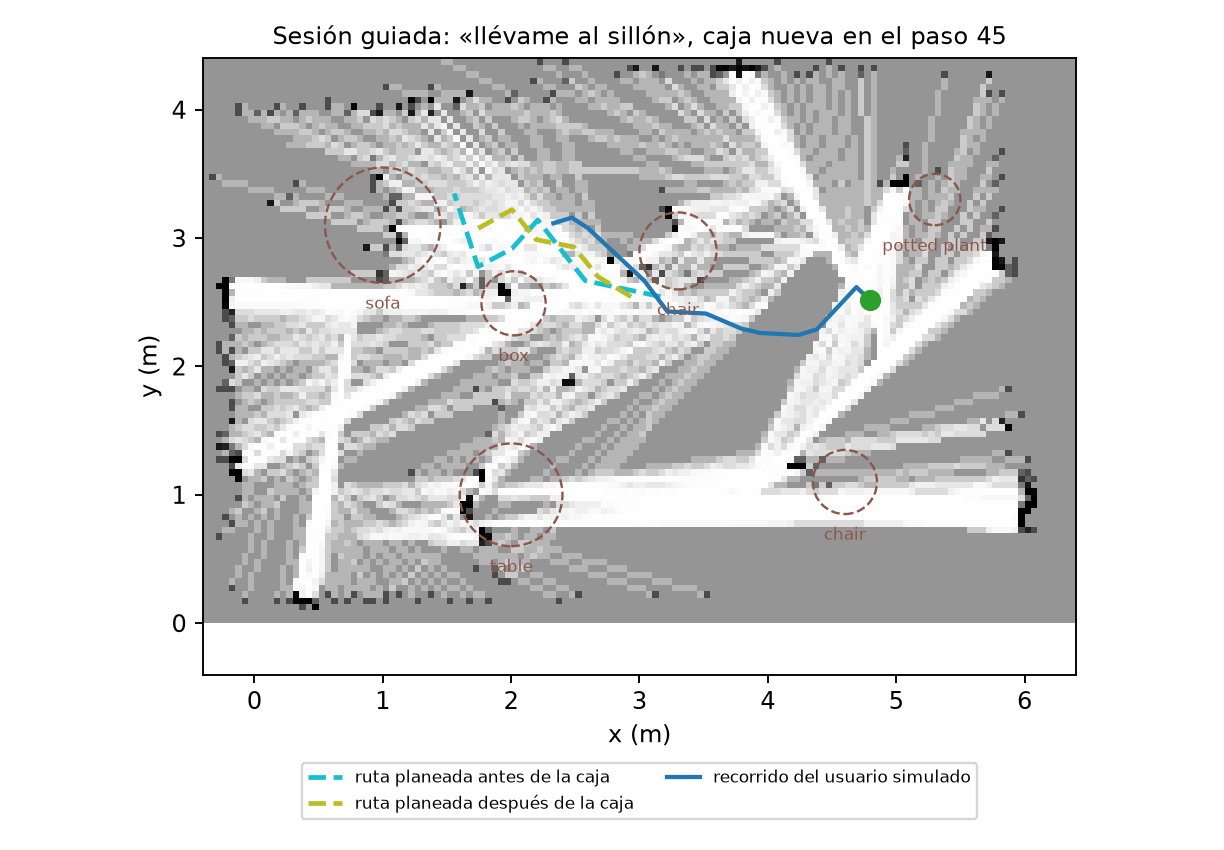
\includegraphics[width=0.82\textwidth]{Capturas_TT2/nav/nav_sesion_ok.png}
    \caption{Sesión en lazo cerrado con una caja que aparece en el camino. Las líneas
    discontinuas son las rutas que calculó el planificador antes y después de la
    caja.}
    \label{fig:nav_sesion}
\end{figure}

La Figura~\ref{fig:nav_vivo} muestra la vista de ruta de la interfaz de
\texttt{main\_nav\_lap.py} en dos momentos de esa sesión. En la segunda captura se
aprecia otro efecto del SLAM: el mapa ligero contiene \emph{landmarks} duplicados
(dos mesas y dos sillones en un cuarto que tiene uno de cada uno).

\begin{figure}[H]
    \centering
    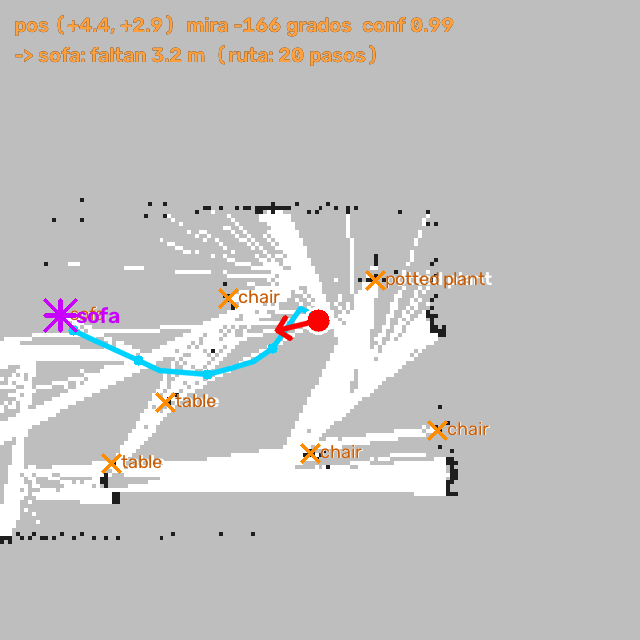
\includegraphics[width=0.48\textwidth]{Capturas_TT2/nav/nav_vivo_p10.png}
    \hfill
    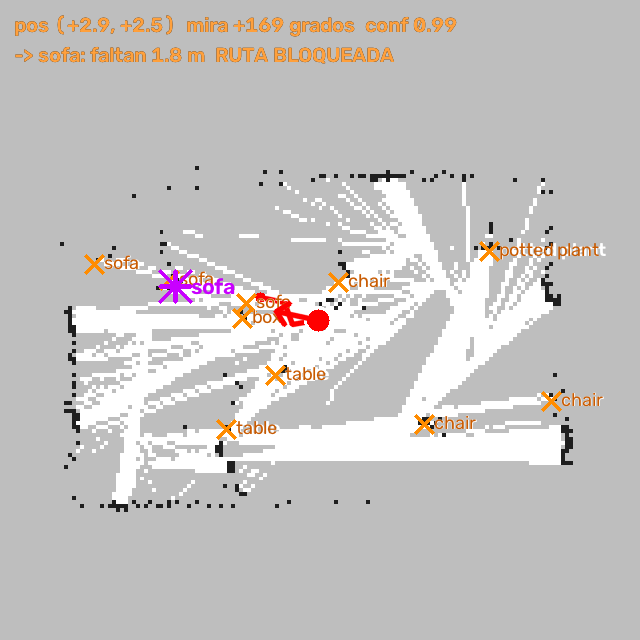
\includegraphics[width=0.48\textwidth]{Capturas_TT2/nav/nav_vivo_p52.png}
    \caption{Vista de ruta en vivo al inicio de la sesión (izquierda) y después de la
    caja (derecha). Cian: ruta planeada; estrella magenta: meta; cruces naranjas:
    \emph{landmarks}.}
    \label{fig:nav_vivo}
\end{figure}

Durante las sesiones se observaron otros dos detalles. Como en la simulación el
agente decide en cada ciclo, el sistema emitió en promedio una indicación cada 1.8
pasos, lo que en uso real sería demasiado; en el dispositivo el ritmo es de una
decisión por segundo y las indicaciones repetidas se agrupan. Además, el mensaje
amigable de llegada dice ``¡Llegamos! Ya estás en sofa'', porque usa la etiqueta en
inglés del \emph{landmark} en lugar del nombre que dijo el usuario.

\textbf{Costo computacional.} Construir la observación toma 0.64~ms, la inferencia
de la política 0.06~ms con Stable-Baselines3 y 0.01~ms con NumPy, y un plan completo
de ruta 7~ms. La navegación no limita la frecuencia del sistema.

\subsection{Limitaciones}

\begin{itemize}
    \item La llegada por percepción se dispara con un solo cuadro y termina sesiones
    antes de tiempo.
    \item Los resultados del 97.8\,\% corresponden al simulador del agente. En lazo
    cerrado con el SLAM y la percepción simulados, la llegada correcta a menos de 1~m
    bajó a 7 de 20 sesiones. Aún no se ha probado con una persona real.
    \item El riesgo por sector se calcula distinto en entrenamiento (a partir de la
    distancia a cualquier obstáculo) y en el sistema real (a partir de las
    detecciones de visión). Se intentó alinear el sistema real con la regla del
    entrenamiento y el desempeño empeoró, por lo que la corrección pendiente es del
    lado del entrenamiento.
    \item La solicitud de ruta alternativa reinicia el seguimiento del progreso, pero no
    obliga al agente a tomar un camino distinto.
    \item Los modelos de ruido del simulador se ajustaron sin los sensores físicos; al
    montar la IMU y los MB1232 habrá que medir el ruido real y reentrenar.
\end{itemize}


% ==============================================================================
\section{Módulo de alertas}
\label{sec:dev_alertas}
% ==============================================================================

\subsection{Descripción}

El módulo de alertas es la capa de seguridad del sistema y corresponde al Algoritmo 7
de TT1. La navegación solo trabaja cuando hay una ruta activa, pero las alertas están
encendidas todo el tiempo, así que una persona puede usar los lentes sin pedir ningún
destino y aun así enterarse de lo que tiene enfrente. El módulo atiende RF-12, RF-20,
RNF-01, RNF-09 y RNF-12.

En cada ciclo, \texttt{alertas.py} lee el cuadro de navegación y regresa la lista de
alertas nuevas, cada una con su prioridad, junto con una bandera que indica si hay que
recalcular la ruta. También se encarga del sonido. Para esa parte se integró el módulo
de pitidos que desarrolló el equipo (\texttt{VozYPLN/alertas.py}), y gracias a él las
alertas no se confunden con las indicaciones de navegación. Una precaución es solo un
pitido estéreo, mientras que una alerta crítica es un pitido seguido de una frase corta
que interrumpe cualquier otra cosa que el sistema esté diciendo.

\subsection{Reglas de alerta}

La Tabla~\ref{tab:alertas_reglas} reúne las reglas. Los umbrales del frente (0.80~m
para la alerta crítica y 1.50~m para la precaución) son los definidos en TT1. En los
costados los umbrales son menores, porque caminar a 60~cm de una pared es lo más normal
en un pasillo y no amerita una alerta crítica. La excepción son las detecciones de
riesgo alto, que usan los umbrales del frente en cualquier sector.

\begin{longtable}{|p{3.4cm}|p{3.6cm}|p{3.2cm}|p{4.3cm}|}
\caption{Reglas del módulo de alertas}
\label{tab:alertas_reglas} \\
\hline
\textbf{Situación} & \textbf{Crítica} & \textbf{Precaución} & \textbf{Ejemplo de
frase} \\
\hline
\endfirsthead
\hline
\textbf{Situación} & \textbf{Crítica} & \textbf{Precaución} & \textbf{Ejemplo de
frase} \\
\hline
\endhead
Obstáculo al frente (mapa o visión) & $< 0.80$~m & $< 1.50$~m & ``Atención:
obstáculo a 80 centímetros al frente. Deténgase.'' \\
\hline
Obstáculo a un costado & $< 0.45$~m & $< 0.80$~m & ``Precaución: obstáculo cerca a
la izquierda.'' \\
\hline
Persona u objeto en movimiento (hasta 2~m) & $< 1.0$~m & de 1.0 a 2.0~m & ``Alto. Se
acerca una persona al frente, muy cerca.'' \\
\hline
Hoyo, agua o escalera al frente (hasta 2.5~m) & $< 1.3$~m & de 1.3 a 2.5~m &
``Atención: un hoyo adelante, a unos 2 pasos.'' \\
\hline
Eco ultrasónico que ninguna detección confirmada explica & $< 0.80$~m & de 0.80 a
1.50~m & ``Atención: pared al frente a 60 centímetros. Deténgase.'' \\
\hline
Detección contradicha por el ultrasonido (al frente) & --- & $< 1.5$~m & ``Posible
silla al frente (solo cámara).'' \\
\hline
Lectura directa de un sensor de proximidad & $< 1.0$~m & de 1.0 a 1.5~m & Pitido
inmediato en la dirección del eco. \\
\hline
\end{longtable}

Si hay una persona en movimiento en un sector, su aviso reemplaza al aviso genérico de
obstáculo de ese sector, para no decir dos cosas sobre lo mismo. Los peligros de piso se
describen en pasos, contando 0.7~m por paso, porque es una medida que el usuario puede
ir contando mientras camina. Las distancias del texto se redondean a múltiplos de
10~cm para que el ruido de la estimación no cambie la frase en cada ciclo, y los objetos
se nombran en español con el mismo diccionario que usa la interacción
(Sección~\ref{sec:dev_interaccion}), de modo que el detector dice \emph{chair} pero el
usuario escucha ``silla''.

Los dos ultrasónicos frontales agregan tres reglas más. Un eco cercano que ninguna
detección confirmada por la cámara explica se avisa como pared u obstáculo; así se
cubren los vidrios, las mamparas y las paredes lisas, que la visión no reconoce. Si los
dos sensores miden casi lo mismo, se trata de una superficie de frente y el aviso dice
``pared''; si solo uno la detecta, el objeto está cargado hacia ese lado. Este aviso
reemplaza al genérico de esa dirección, porque el ultrasonido mide con más precisión que
el mapa. En cambio, una detección visual que el ultrasonido contradice, porque el haz
debería alcanzarla y no hay eco a esa distancia, ya no dispara una alerta crítica con la
distancia de la cámara. Se avisa solo como precaución, con la frase ``posible\dots{}
(solo cámara)'', siguiendo la idea de RNF-09 de avisar sin alarmar de más.

La tercera regla es de rapidez. Las lecturas no esperan al ciclo de visión; la función
\texttt{conectarUltrasonido} revisa cada lectura nueva y, si hay un eco a menos de 1.5~m,
suena un pitido de inmediato en su dirección. Antes se descartan los ecos del piso con
el cabeceo de la IMU, y la lectura mínima del sensor, 20~cm, se interpreta como ``20~cm
o menos'' y produce un pitido crítico, porque es la situación más peligrosa. La alerta
correspondiente llega al navegador en el siguiente ciclo. Como los dos sensores se
disparan por turnos y cada medición toma 100~ms, cada uno se actualiza unas cinco veces
por segundo.

\subsection{Dosificación y recálculo}

Si una alerta se repitiera en cada ciclo, el usuario recibiría diez avisos por segundo.
Para evitarlo, cada alerta tiene un tiempo de espera antes de volver a sonar, de 2.5~s
para las críticas y de 8~s para las precauciones. El tiempo se cuenta por prioridad,
por dirección (frente, izquierda o derecha) y por tipo de aviso (obstáculo, persona en
movimiento o peligro de piso), de modo que una precaución por algo a la izquierda no
silencia una precaución por algo al frente.

Esta forma de agrupar se definió después de dos intentos. Primero, el tiempo de espera
se aplicaba al texto exacto de la frase, pero como la distancia cambia de un ciclo a
otro, cada frase resultaba ``nueva'' y no se filtraba nada. Después se agrupó por el
inicio del texto, y en las pruebas del escenario que se describe más adelante una
precaución lateral llegó a silenciar durante 8~s la precaución frontal de una pared.

Cualquier alerta crítica activa la bandera de recálculo. El navegador la recibe y decide
en ese mismo ciclo, sin esperar su intervalo de un segundo, y el planificador de ruta
recalcula de inmediato. Las alertas se pueden apagar y encender con la tecla \texttt{x}
en la computadora portátil y con un doble clic del botón físico en el prototipo.

\subsection{Pitidos estéreo}

El módulo de pitidos del equipo genera los tonos por software y los reproduce en un hilo
propio, de modo que suenan aunque el programa principal esté escuchando o hablando. La
dirección se codifica con el balance entre canales; un obstáculo a la izquierda suena
fuerte en el oído izquierdo y bajito en el derecho, y uno al frente suena igual en ambos.
El nivel se codifica con el patrón (Figura~\ref{fig:alertas_pitidos}). La alerta
crítica son cuatro tonos cortos que alternan entre 2100 y 1500~Hz, y la precaución, dos
tonos de 1200~Hz más largos. Mientras suena un pitido la cola de voz espera, y si llega
una alerta crítica mientras el sistema habla, la frase en curso se corta.

\begin{figure}[H]
    \centering
    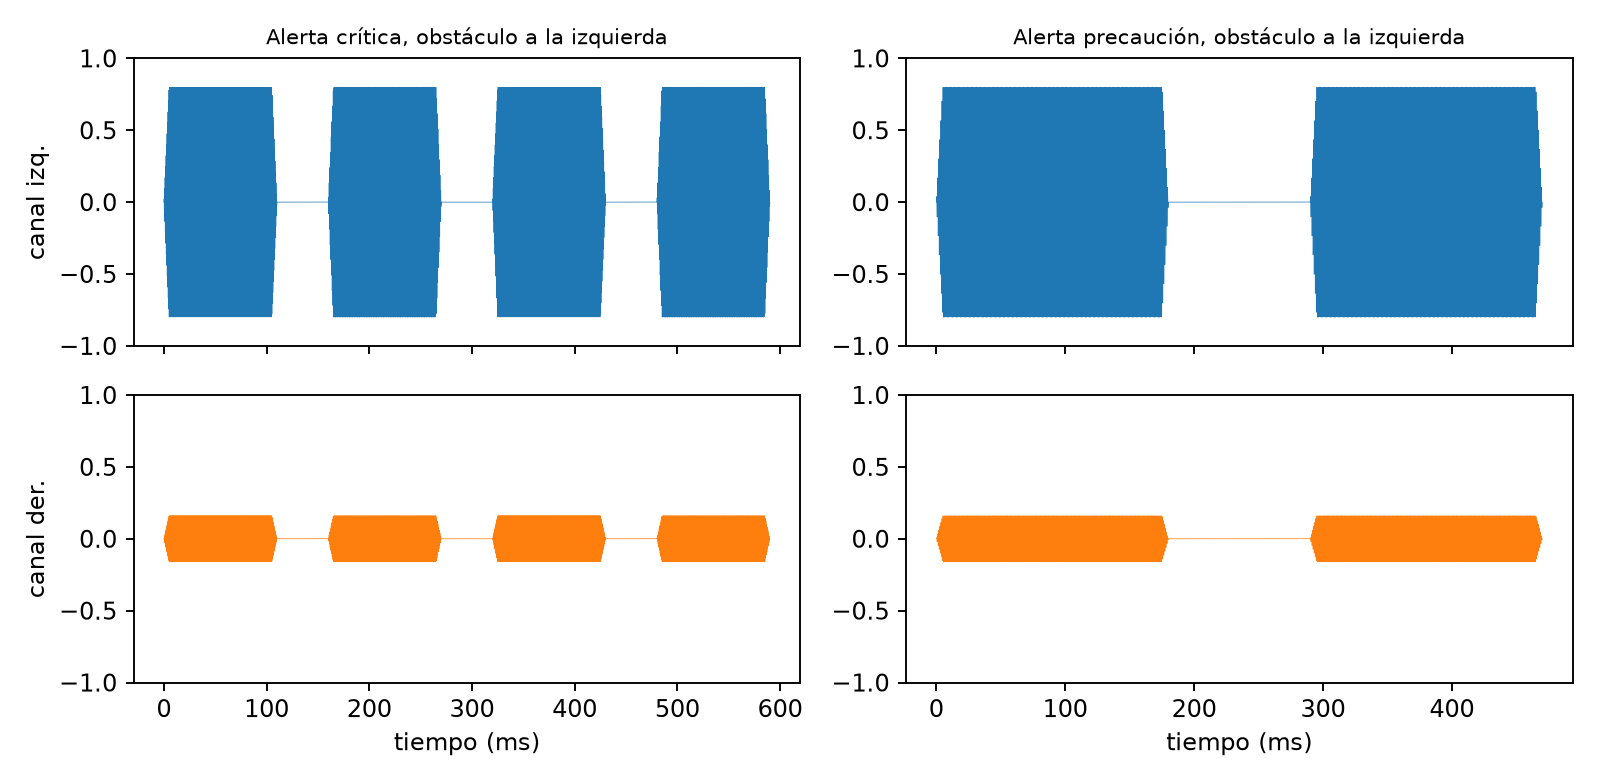
\includegraphics[width=0.88\textwidth]{Capturas_TT2/nav/alertas_pitidos.png}
    \caption{Forma de onda de los pitidos para un obstáculo a la izquierda, con la alerta
    crítica a la izquierda y la precaución a la derecha. El canal derecho suena al
    20\,\% del volumen del izquierdo.}
    \label{fig:alertas_pitidos}
\end{figure}

El módulo del equipo trae también su propia lógica para decidir el nivel; por ejemplo,
un vehículo a menos de 5~m es crítico, y si un sensor y la cámara reportan lo mismo en la
misma dirección casi al mismo tiempo, la alerta sube un nivel. En el sistema integrado
esa lógica no se usa, porque el nivel lo decide \texttt{alertas.py} con las reglas de la
Tabla~\ref{tab:alertas_reglas} y el módulo del equipo solo se encarga de sonar.

\subsection{Resultados}

\textbf{Pruebas con el prototipo.} \TODO{escenarios probados con el prototipo (por
ejemplo, acercarse a una pared, a una puerta de vidrio y a una persona), alertas
esperadas contra alertas emitidas, falsas alarmas y si los participantes distinguieron
la dirección de los pitidos}.

\textbf{Escenario simulado.} Para revisar el comportamiento de las reglas se preparó un
escenario en el cuarto simulado, en el que el usuario camina en línea recta hacia la
pared del fondo mientras una persona le cruza por delante. La
Figura~\ref{fig:alertas_escenario} muestra la distancia libre al frente según el mapa,
la distancia estimada a la persona y las alertas que emitió el módulo, 14 en total en
17~s.

\begin{figure}[H]
    \centering
    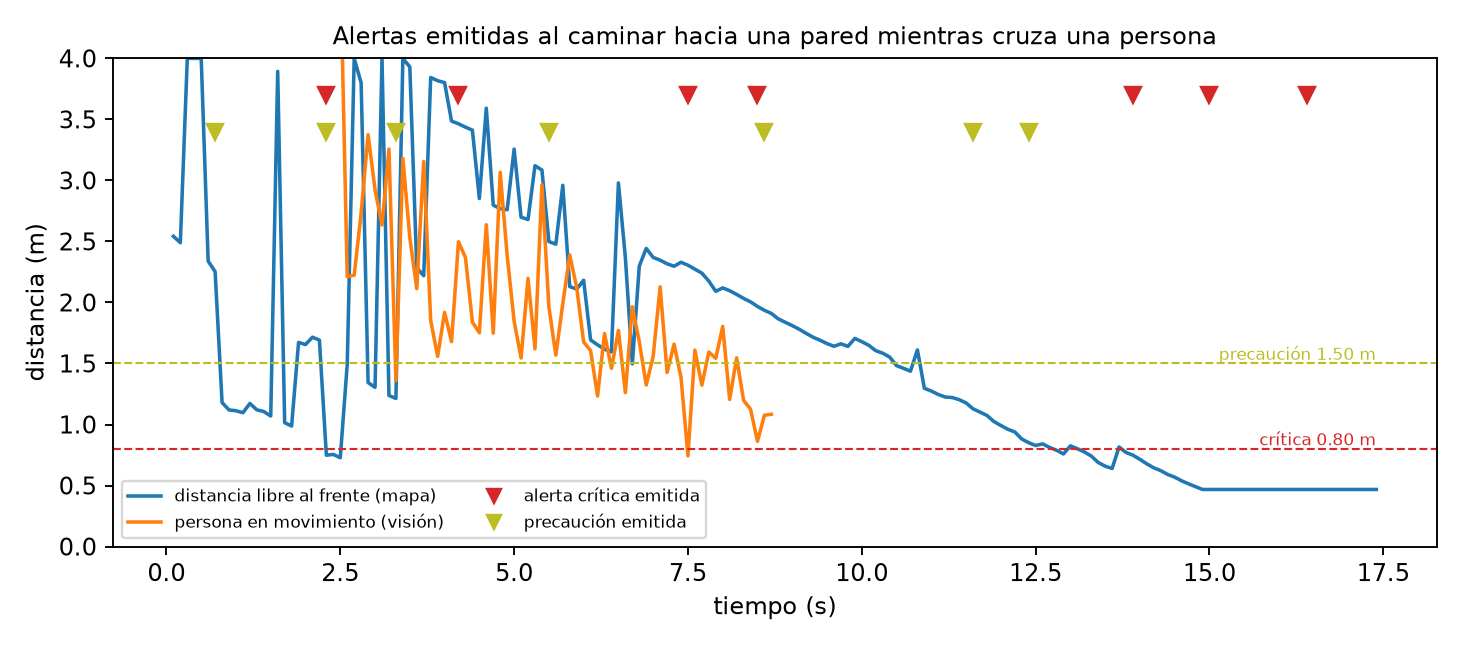
\includegraphics[width=\textwidth]{Capturas_TT2/nav/alertas_escenario.png}
    \caption{Alertas emitidas en el escenario de prueba. Los triángulos marcan cada alerta
    crítica (rojo) y cada precaución (verde).}
    \label{fig:alertas_escenario}
\end{figure}

La persona se avisó como se esperaba. A los 3.3~s, ya a menos de 2~m, sonó ``Precaución:
una persona en movimiento al frente'', y a los 7.5~s, a menos de 1~m, la alerta crítica
``Alto. Se acerca una persona al frente, muy cerca''. Al seguir su camino, la persona
quedó del lado derecho del usuario y el aviso cambió de dirección (8.5~s). Después el
ultrasonido detectó la pared, primero con precauciones a los 11.6 y 12.4~s y luego con
alertas críticas a los 13.9, 15.0 y 16.4~s, la última a 51~cm, porque el usuario siguió
avanzando. Entre los 12.6 y los 13.9~s el mapa ya marcaba menos de 0.80~m, pero el eco,
que mide la distancia real, todavía estaba por encima del umbral; como el aviso del
ultrasonido reemplaza al del mapa en esa dirección, la alerta crítica esperó a que el
eco bajara.

La prueba dejó ver dos efectos que conviene tener presentes. El primero es que el
cálculo estéreo del lado oscila cuando el usuario se acerca a una pared con un ligero
ángulo, de modo que la misma pared se reporta unas veces ``al frente'' y otras
``adelante a la derecha''. Como la dosificación cuenta cada dirección por separado, eso
produjo cinco avisos por la misma pared en menos de cinco segundos. \TODO{agrupar los
avisos del ultrasonido en una sola dirección frontal cuando ambos sensores ven la misma
superficie}. El segundo es que al inicio sonaron alertas por la mesa y el sillón que
quedaban a los lados, algunas con una distancia menor a la real. El escenario parte de un
mapa construido en un recorrido previo y la pose inicial se fijó a mano, así que hay un
desajuste entre la pose y el mapa; en una corrida de prueba se comprobó que, con la pose
desplazada 0.4~m, una pared ya registrada aparecía a 40~cm en un costado donde no había
nada.

En cuanto al tiempo, evaluar las reglas toma en promedio 0.007~ms por ciclo, así que lo
que tarda una alerta en sonar desde que el obstáculo aparece en la imagen depende de la
visión, unos 160~ms por cuadro en la computadora portátil. En el prototipo esa latencia
es de \TODO{latencia de alerta medida en la Raspberry Pi}, contra los 2~s que permite
RNF-01. El módulo tiene 26 pruebas automatizadas junto con el planificador de ruta.

\subsection{Limitaciones}

Las alertas heredan los errores de la percepción. Un tapete detectado como hoyo provoca
una alerta falsa, y un obstáculo que la cámara no reconoce y que no devuelve eco, como
un objeto bajo y muy cercano, no provoca ninguna. Tampoco hay alertas para lo que queda
detrás o muy a los costados del usuario, porque ni la cámara ni los ultrasónicos cubren
esas zonas.


% ==============================================================================
\section{Módulos de interacción: voz, PLN y salida}
\label{sec:dev_interaccion}
% ==============================================================================

\subsection{Descripción}

Los módulos de interacción son la única interfaz entre el usuario y el sistema. El
usuario habla, el sistema transcribe lo que dijo, interpreta la intención y responde
en voz alta; ninguna función requiere ver una pantalla ni tocar un botón, salvo el
botón opcional para apagar las alertas. Estos módulos atienden RF-01 a RF-06 y los
requerimientos no funcionales RNF-02, RNF-07, RNF-10 y RNF-11.

El reconocimiento de voz, el procesamiento de lenguaje natural (PLN), la personalidad
del asistente y la síntesis de voz los desarrolló el equipo en la carpeta
\texttt{VozYPLN/}. El trabajo de integración consistió en conectar esas piezas con el
navegador y con las alertas en \texttt{interaccion.py}. La Tabla~\ref{tab:inter_partes}
resume los componentes.

\begin{table}[H]
\centering
\caption{Componentes de los módulos de interacción}
\label{tab:inter_partes}
\renewcommand{\arraystretch}{1.25}
\begin{tabular}{|p{3.6cm}|p{10.9cm}|}
\hline
\textbf{Componente} & \textbf{Función} \\
\hline
\texttt{voz\_recog.py} & Reconocimiento de voz sin conexión con Vosk (modelo
\texttt{vosk-model-small-es-0.42}) a 16~kHz. \\
\hline
\texttt{PLN\_oneimport.py} & Clasificación de la intención y extracción del destino. \\
\hline
\texttt{dialogo.py} & Frases con la personalidad del asistente (``Guía''). \\
\hline
\texttt{Tts.py} & Síntesis de voz con edge-tts (voz \texttt{es-MX-DaliaNeural}) y respaldo
local con pyttsx3. \\
\hline
\texttt{interaccion.py} & Integración: cola de voz con prioridades, escucha en segundo
plano y traducción de intenciones a comandos del navegador. \\
\hline
\end{tabular}
\end{table}

Respecto al diseño de TT1 hubo tres cambios. El detector de actividad de voz y el
filtro de Wiener que se habían planteado como etapas previas no se implementaron por
separado: Vosk detecta por sí mismo el final de cada frase y el filtro no mejoró el
reconocimiento en las primeras pruebas. El PLN no usa spaCy, sino un clasificador
propio escrito en Python puro, que combina reglas con una red neuronal pequeña. Y la
síntesis de voz usa una voz neuronal en línea con un respaldo local, en lugar de
depender solo de pyttsx3.

\subsection{Reconocimiento de voz}

El reconocedor captura audio del micrófono en bloques de 0.25~s y los entrega a Vosk.
Cuando Vosk detecta que la frase terminó, devuelve el texto y el reconocedor lo coloca
en una cola que el ciclo principal revisa en cada cuadro. La escucha corre en un hilo
aparte, de modo que el sistema sigue percibiendo y navegando mientras espera una
orden. Mientras el sistema habla, lo que capta el micrófono se descarta, porque lo más
probable es que se esté escuchando a sí mismo. Si no hay micrófono o falta el modelo de
Vosk, el sistema lo avisa y acepta las órdenes por teclado, lo cual se usa durante el
desarrollo.

\subsection{Procesamiento de lenguaje natural}

El PLN recibe el texto transcrito y devuelve una de 14 intenciones, el destino si lo
hay, un valor de confianza y una respuesta sugerida. Las intenciones son: destino,
pausa, reanudar, detener, ruta alternativa, emergencia, ubicación, entorno, repetir,
cancelar, ayuda, confirmar, negar y estado de la ruta. El proceso tiene cuatro pasos:

\begin{enumerate}
    \item \textbf{Normalización.} El texto se pasa a minúsculas, se quitan los acentos
    y los signos, y se divide en palabras. Se descartan palabras sin contenido (``el'',
    ``por favor'') y se agregan sinónimos conocidos.
    \item \textbf{Palabras de seguridad.} Si el texto contiene una palabra como
    ``detente'', ``alto'', ``auxilio'' o ``cancela'', la intención se fija de inmediato
    con confianza de 0.99, sin consultar a los clasificadores.
    \item \textbf{Clasificación.} Se calculan dos puntuaciones para cada intención. La
    de reglas compara el texto con 121 frases de referencia mediante similitud de
    palabras basada en la distancia de Levenshtein, que tolera errores del
    reconocedor, y similitud de coseno entre bolsas de palabras. La de la red neuronal
    usa una capa oculta de 24 neuronas sobre un vector TF-IDF, entrenada con 164
    ejemplos (las frases de referencia más variantes con sinónimos). Ambas se combinan
    con un peso para la red que crece con el número de ejemplos aprendidos y con la
    proporción de palabras del texto que la red conoce. Si la mejor puntuación es
    menor que 0.42, o si las dos mejores quedan casi empatadas, el resultado es
    ``desconocido'' y el sistema pide repetir.
    \item \textbf{Destino.} Para la intención de destino se busca primero un lugar
    conocido por similitud, después lo que sigue a frases como ``llévame a'' o
    ``quiero ir a'' y, como último recurso, las palabras que quedan al quitar las de
    navegación. Si no hay destino, el sistema pregunta ``¿A dónde te gustaría ir?'' y
    toma la siguiente frase como respuesta.
\end{enumerate}

El PLN puede aprender frases nuevas cuando recibe una corrección, y las guarda en un
archivo local. Para la evaluación de esta sección se usó el modelo sin frases
aprendidas, que es el que tendría un usuario nuevo.

\subsection{Integración con el navegador}

La clase \texttt{Interaccion} convierte cada intención en una acción. Las de la
sesión (destino, pausa, reanudar, detener, cancelar, ruta alternativa, ubicación y
estado) se envían al navegador como comandos. El destino se limpia antes de enviarlo
(se quitan artículos y plurales, porque el PLN puede devolver ``la puerta'' o
``baños'') y se traduce a la etiqueta del \emph{landmark} con un diccionario de
sinónimos: ``salida'', ``puerta'' y ``entrada'' se buscan como \emph{door}; ``baño''
como \emph{toilet}; ``escritorio'' como \emph{desk}, y así para 38 palabras. Las demás
intenciones se resuelven en la misma clase:

\begin{itemize}
    \item \textbf{Entorno} (``¿qué hay enfrente?''): describe el objeto más cercano en
    cada sector, o la distancia libre si no hay ninguno. La frase tiene la forma ``Al
    frente, door a 2 metros. A la izquierda libre. A la derecha, chair a 90
    centímetros'': el nombre del objeto se dice con la etiqueta en inglés del
    detector, lo cual es una deficiencia pendiente.
    \item \textbf{Repetir}: vuelve a decir la última indicación de navegación.
    \item \textbf{Emergencia}: emite un aviso con prioridad máxima y pausa la
    navegación. El aviso a un contacto de emergencia quedó pendiente.
    \item \textbf{Ayuda}: enumera lo que se puede decir.
\end{itemize}

Las frases ``apagar sistema'' y ``terminar programa'' cierran el sistema con una
despedida.

\subsection{Salida de voz}

Todo lo que el sistema dice pasa por una cola con tres prioridades: 0 para alertas, 1
para indicaciones de navegación y 2 para respuestas y confirmaciones. Un mensaje de
prioridad 0 interrumpe lo que se esté diciendo. Las indicaciones de navegación forman
un canal especial en el que solo se dice la más reciente: si el sintetizador va
atrasado y en la cola hay un ``gire a la izquierda'' viejo, se descarta, porque ya no
corresponde a la posición del usuario; también se descartan las indicaciones que
llevan más de 6~s esperando. Mientras suena un pitido de alerta, la cola espera.

La síntesis usa edge-tts con la voz neuronal \texttt{es-MX-DaliaNeural}, que suena
natural pero necesita conexión a internet. Cada frase sintetizada se guarda en un
archivo, así que las frases repetidas (que son la mayoría) se reproducen sin conexión.
Si la conexión falla, el sistema cambia a pyttsx3, que usa la voz instalada en el
sistema operativo; si tampoco está disponible, escribe las frases en consola.

\subsection{Personalidad del asistente}

El navegador genera las frases literales definidas en TT1 (``Avance 3 metros'',
``Gire ligeramente a la izquierda''). Con el modo amigable activado, que es el
predeterminado, \texttt{dialogo.py} las reformula con un tono más cercano: la
distancia se expresa en pasos, los giros con referencias cotidianas y las frases
varían para no sonar repetitivas (Tabla~\ref{tab:inter_frases}). La frase
``Deténgase'' y las alertas no se reformulan, porque en esos casos importa más la
rapidez que la amabilidad.

\begin{table}[H]
\centering
\caption{Frases literales del navegador y su versión amigable}
\label{tab:inter_frases}
\renewcommand{\arraystretch}{1.25}
\begin{tabular}{|p{5.2cm}|p{9.3cm}|}
\hline
\textbf{Literal (TT1)} & \textbf{Amigable (dialogo.py)} \\
\hline
Ruta calculada. Iniciando navegación. & Muy bien, te llevo a sillon. Vamos paso a
paso. \\
\hline
Gire ligeramente a la izquierda & Perfecto, da una vuelta suave a tu izquierda. \\
\hline
Gire a la derecha 90 grados & Listo, da vuelta completa a tu derecha, como una
esquina. \\
\hline
Avance 3 metros & Vas muy bien, continúa de frente unos 4 pasos. \\
\hline
Ha llegado a su destino. & ¡Listo, llegamos a door! \\
\hline
Deténgase & Deténgase (sin cambio) \\
\hline
\end{tabular}
\end{table}

Una sutileza de la integración: \texttt{dialogo.py} considera positivos los giros a la
derecha, mientras que en el resto del sistema los ángulos positivos son hacia la
izquierda. La conversión invierte el signo; las pruebas automatizadas verifican que
un giro a la izquierda del navegador se diga ``a tu izquierda''.

El Algoritmo~\ref{alg:dev_inter} resume el manejo de una frase del usuario.

\begin{center}
\captionof{algorithm}{Manejo de una frase del usuario}
\label{alg:dev_inter}
\end{center}
\vspace{-1.8cm}
\rule{\textwidth}{0.4pt}
\vspace{-0.9cm}
\begin{algorithmic}[1]

\Statex \textbf{ENTRADA:} texto (de Vosk o del teclado), cuadro\_nav
\Statex \textbf{SALIDA:} mensajes para la cola de voz

\Statex
\If{texto es ``apagar sistema'' o ``terminar programa''}
    \State \Return [despedida]
\EndIf
\If{se esperaba la respuesta a ``¿a dónde te gustaría ir?''}
    \State texto $\gets$ ``llévame a '' + texto
\EndIf
\State r $\gets$ PLN.procesar(texto)
\If{r.intención = destino}
    \If{no hay destino}
        \State marcar que se espera respuesta
        \State \Return [``¿A dónde te gustaría ir?'']
    \EndIf
    \State etiqueta $\gets$ sinónimos(limpiar(r.destino))
    \State msgs $\gets$ navegador.comando(navegar, etiqueta, cuadro\_nav)
\ElsIf{r.intención es de sesión}
    \State msgs $\gets$ navegador.comando(r.intención)
\ElsIf{r.intención = entorno}
    \State msgs $\gets$ [describir\_entorno(cuadro\_nav)]
\ElsIf{r.intención = emergencia}
    \State msgs $\gets$ [aviso con prioridad 0] + navegador.comando(pausa)
\Else
    \State msgs $\gets$ [respuesta según la intención]
\EndIf
\If{modo amigable}
    \State reformular las confirmaciones con dialogo.py
\EndIf
\State \Return msgs

\end{algorithmic}
\vspace{-0.9cm}
\rule{\textwidth}{0.4pt}

\subsection{Resultados}

\textbf{Evaluación del PLN.} Para medir el PLN con frases que no conociera, se
redactó un conjunto de 102 frases de prueba, distintas de las frases de referencia,
con la intención correcta de cada una (por ejemplo, ``espérame tantito'' para pausa o
``ya no quiero seguir'' para detener). El conjunto se escribió antes de correr la
evaluación y no se modificó después de ver los resultados. El PLN acertó la intención
en 80 de las 102 frases (78.4\,\%). En las frases de destino, extrajo correctamente
el lugar en 16 de 21. Procesar una frase tomó en promedio 2.8~ms (máximo 7~ms). La
Figura~\ref{fig:pln_confusion} muestra la matriz de confusión.

\begin{figure}[H]
    \centering
    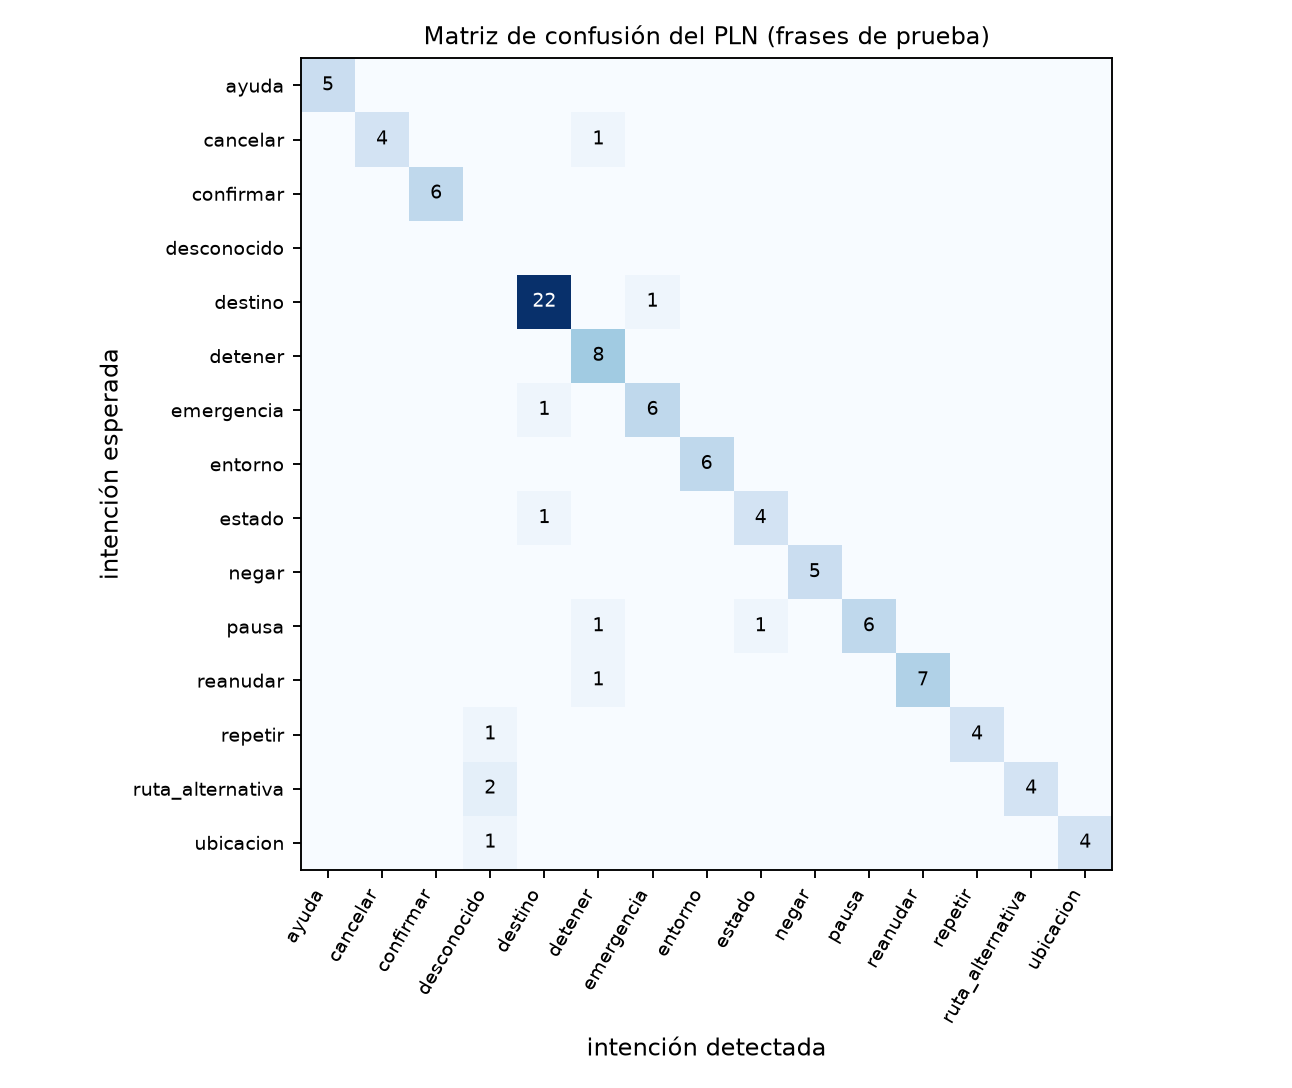
\includegraphics[width=0.78\textwidth]{Capturas_TT2/voz/pln_confusion.png}
    \caption{Matriz de confusión del PLN sobre las 102 frases de prueba.}
    \label{fig:pln_confusion}
\end{figure}

La mayoría de los errores son inofensivos: la frase cae en ``desconocido'' y el
sistema pide repetir, o el destino se extrae con palabras de sobra (``llevas banca'',
``guiar mesa''), lo que hace que no se encuentre el lugar. Algunos, sin embargo, son
delicados por su efecto sobre la navegación:

\begin{itemize}
    \item ``ya no quiero seguir'' se interpretó como reanudar, y ``termina la
    navegación'' como pausa;
    \item ``no es correcto'' se interpretó como confirmar;
    \item ``ayuda'' se interpretó como emergencia y, al revés, ``ayuda, me caí'' como
    una petición de ayuda sobre los comandos;
    \item ``detente un momento por favor'' se interpretó como detener en lugar de
    pausa, por la palabra de seguridad ``detente''. Esta última es una decisión de
    diseño conservadora y se considera aceptable.
\end{itemize}

\textbf{Reconocimiento de voz con ruido.} Para evaluar la cadena completa sin
voluntarios se generó audio con las 10 voces en español disponibles en macOS (dos
voces naturales, Paulina y Mónica, y ocho voces de estilo caricaturesco) diciendo 30
comandos de uso frecuente. Cada audio se pasó por Vosk y por el PLN en limpio y
mezclado con ruido rosa a 20, 10 y 5~dB de relación señal a ruido. Un comando cuenta
como correcto si produce la acción esperada y, en los de destino, el lugar correcto.
Los resultados se muestran en la Tabla~\ref{tab:asr} y en la
Figura~\ref{fig:asr_ruido}.

\begin{table}[H]
\centering
\caption{Voz sintetizada, Vosk y PLN (300 audios por condición)}
\label{tab:asr}
\renewcommand{\arraystretch}{1.2}
\begin{tabular}{|l|c|c|c|}
\hline
\textbf{Condición} & \textbf{WER} & \textbf{Comandos correctos} &
\textbf{Correctos, voces naturales} \\
\hline
Limpio & 22.2\,\% & 80.0\,\% & 91.7\,\% \\
20~dB & 23.8\,\% & 78.3\,\% & 81.7\,\% \\
10~dB & 33.0\,\% & 71.0\,\% & 63.3\,\% \\
5~dB & 43.1\,\% & 58.7\,\% & 45.0\,\% \\
\hline
\end{tabular}
\end{table}

\begin{figure}[H]
    \centering
    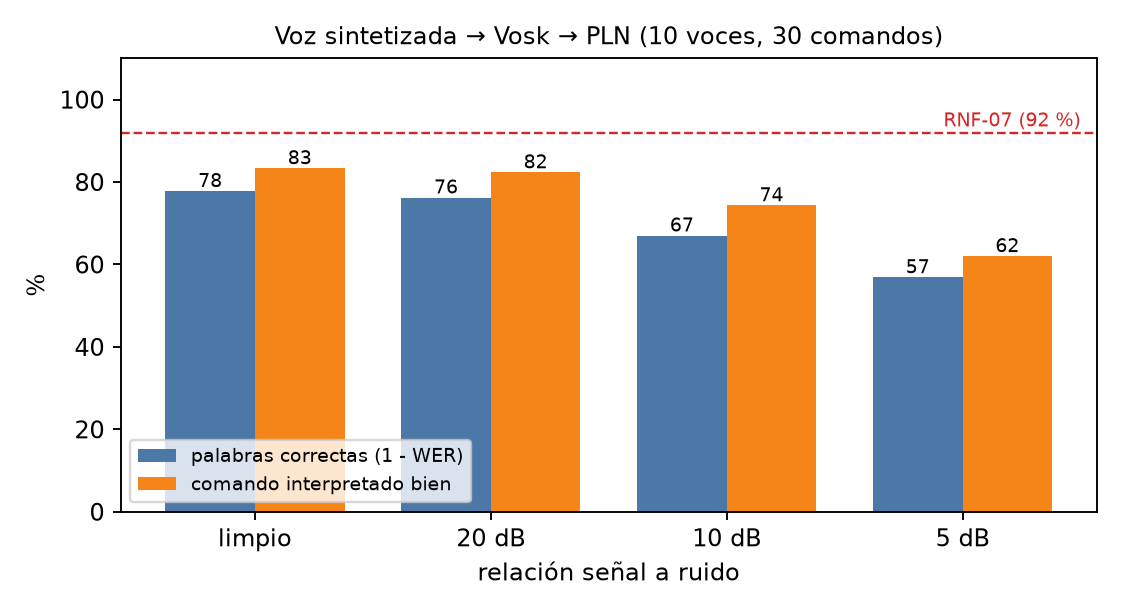
\includegraphics[width=0.75\textwidth]{Capturas_TT2/voz/asr_ruido.png}
    \caption{Palabras correctas y comandos bien interpretados según el nivel de ruido.}
    \label{fig:asr_ruido}
\end{figure}

En audio limpio con las voces naturales el sistema interpreta bien el 91.7\,\% de los
comandos, prácticamente en el 92\,\% que pide RNF-07. Con ruido el desempeño cae
rápido. Una voz hablada a corta distancia del micrófono en un entorno de 60~dB
(el nivel que menciona RNF-07) equivale aproximadamente a la franja de 5 a 10~dB de la
tabla, donde los comandos correctos están entre 59 y 71\,\%. Por lo tanto, el
requerimiento no se cumple en condiciones ruidosas. También se observó que, en los
194 audios limpios que Vosk transcribió sin ningún error, el PLN acertó en 181
(93\,\%); el resto del error en limpio proviene del reconocimiento.

En cuanto a la latencia, una vez que termina el audio Vosk entrega el resultado final
en 8~ms en promedio (17~ms en el percentil 95) y el PLN tarda 2~ms. Esta medición no
incluye el tiempo que Vosk espera en silencio para decidir que la frase terminó,
que en uso real se suma a la latencia percibida. Aun así, el procesamiento queda muy
por debajo de los 500~ms de RNF-02.

Las pruebas automatizadas de la interacción (24) verifican la traducción de
intenciones a comandos, la aclaración de destino en dos turnos, la limpieza de
destinos, la conversión de signo de los giros, la descripción del entorno y el
funcionamiento sin micrófono ni sintetizador.

\subsection{Limitaciones}

\begin{itemize}
    \item El PLN acierta el 78\,\% de las frases nuevas y comete errores que invierten el
    sentido de la orden (detener interpretado como reanudar). Ampliar las frases de
    referencia con las formas que usan las personas y revisar las palabras de seguridad
    son los pasos inmediatos.
    \item Con ruido de calle, el reconocimiento queda lejos del 92\,\% de RNF-07.
    \item La evaluación de voz usó voces sintéticas; falta probar con personas reales,
    con distintos acentos y con el micrófono del prototipo.
    \item La voz neuronal requiere internet la primera vez que se dice cada frase; sin
    conexión se usa una voz del sistema mucho menos natural.
    \item La llegada y la descripción del entorno mencionan las etiquetas en inglés
    del detector (``llegamos a door'', ``chair a 90 centímetros''). Hace falta un
    diccionario inverso de etiquetas a nombres en español.
    \item El aviso a un contacto de emergencia no está implementado.
\end{itemize}

